% !TeX document-id = {3ccf434d-8187-4348-af82-ed6ccf391a39}
% !TEX TS-program = XeLaTeX
% Commands for running this example:
% 	 xelatex main
% 	 bibtex8 -W -c cp1256fa main
%      xindy -L persian -C utf8 -M texindy main
% 	 xelatex main
% 	 xelatex main
% End of Commands

\documentclass[oneside,openany,bsc]{IUST-Thesis}

% در این فایل، دستورها و تنظیمات مورد نیاز، آورده شده است.
%-------------------------------------------------------------------------------------------------------------------

\usepackage{array}
\newcolumntype{P}[1]{>{\centering\arraybackslash}p{#1}}

\usepackage{tabularx}

\usepackage[thinlines]{easytable}

\usepackage{enumitem}

\usepackage{booktabs}

\usepackage{titlesec}

\usepackage[numbers]{natbib}

\usepackage{totcount}
\regtotcounter{chapter}

\usepackage[usenames,dvipsnames]{color,xcolor}

\usepackage{listings}
\usepackage{listings-golang} % import this package after listings

\definecolor{dkgreen}{rgb}{0,0.6,0}
\definecolor{gray}{rgb}{0.5,0.5,0.5}
\definecolor{mauve}{rgb}{0.58,0,0.82}

\lstset{frame=tb,
  language=Golang,
  aboveskip=3mm,
  belowskip=3mm,
  showstringspaces=false,
  columns=flexible,
  basicstyle={\linespread{1}\small\ttfamily},
  numbers=none,
  numberstyle=\tiny\color{gray},
  keywordstyle=\color{blue},
  commentstyle=\color{dkgreen},
  stringstyle=\color{mauve},
  breaklines=true,
  breakatwhitespace=true,
  tabsize=3
}

% در ورژن جدید زی‌پرشین برای تایپ متن‌های ریاضی، این سه بسته، حتماً باید فراخوانی شود
\usepackage{amsthm,amssymb,amsmath}
% بسته‌ای برای تنطیم حاشیه‌های بالا، پایین، چپ و راست صفحه
\usepackage[top=40mm, bottom=40mm, left=25mm, right=35mm]{geometry}
% بسته‌‌ای برای ظاهر شدن شکل‌ها و تصاویر متن
\usepackage{graphicx}
% بسته‌ای برای رسم کادر
\usepackage{framed} 
% بسته‌‌ای برای چاپ شدن خودکار تعداد صفحات در صفحه «معرفی پایان‌نامه»
\usepackage{lastpage}
% بسته‌ و دستوراتی برای ایجاد لینک‌های رنگی با امکان جهش
\usepackage[pagebackref=false,colorlinks,linkcolor=blue,citecolor=blue]{hyperref}
% چنانچه قصد پرینت گرفتن نوشته خود را دارید، خط بالا را غیرفعال و  از دستور زیر استفاده کنید چون در صورت استفاده از دستور زیر‌‌، 
% لینک‌ها به رنگ سیاه ظاهر خواهند شد که برای پرینت گرفتن، مناسب‌تر است
%\usepackage[pagebackref=false]{hyperref}
% بسته‌ لازم برای تنظیم سربرگ‌ها
\usepackage{fancyhdr}
%
\usepackage{setspace}
\usepackage{algorithm}
% \usepackage{algorithmic}
\usepackage[noend]{algpseudocode}
\usepackage{subfigure}
\usepackage[subfigure]{tocloft}


% بسته‌ای برای ظاهر شدن «مراجع» و «نمایه» در فهرست مطالب
\usepackage[nottoc]{tocbibind}

% دستورات مربوط به ایجاد نمایه
\usepackage{makeidx}
\makeindex
%%%%%%%%%%%%%%%%%%%%%%%%%%
% فراخوانی بسته زی‌پرشین و تعریف قلم فارسی و انگلیسی
\usepackage[extrafootnotefeatures]{xepersian}
% \settextfont[Scale=1]{XBNiloofar.ttf}
\settextfont[Scale=1,BoldFont={*Bold}]{IRNazanin.ttf}
\setlatintextfont[Scale=1]{IRNazanin.ttf}
% \setlatintextfont[Scale=0.9]{Times New Roman}

%%%%%%%%%%%%%%%%%%%%%%%%%%
% چنانچه می‌خواهید اعداد در فرمول‌ها، انگلیسی باشد، خط زیر را غیرفعال کنید
% \setdigitfont[Scale=1]{XBZar.ttf}%{Persian Modern}
%%%%%%%%%%%%%%%%%%%%%%%%%%
% تعریف قلم‌های فارسی و انگلیسی اضافی برای استفاده در بعضی از قسمت‌های متن
% \defpersianfont\titlefont[Scale=1]{bnaz.ttf}
\defpersianfont\titlefont[Scale=1]{IRNazanin.ttf}
% \defpersianfont\titlefont[Scale=1]{XBNiloofar.ttf}
% \defpersianfont\iranic[Scale=1.1]{XB Zar Oblique}%Italic}%
% \defpersianfont\nastaliq[Scale=1.2]{IranNastaliq}

%%%%%%%%%%%%%%%%%%%%%%%%%%
% دستوری برای حذف کلمه «چکیده»
% \renewcommand{\abstractname}{}
% دستوری برای حذف کلمه «abstract»
%\renewcommand{\latinabstract}{}
% دستوری برای تغییر نام کلمه «اثبات» به «برهان»
\renewcommand\proofname{\textbf{برهان}}
% دستوری برای تغییر نام کلمه «کتاب‌نامه» به «مراجع»
\renewcommand{\bibname}{مراجع}
% دستوری برای تعریف واژه‌نامه انگلیسی به فارسی
\newcommand\persiangloss[2]{\lr{#2}\dotfill#1\\}
% دستوری برای تعریف واژه‌نامه فارسی به انگلیسی 
\newcommand\englishgloss[2]{#2\dotfill\lr{#1}\\}
% تعریف دستور جدید «\پ» برای خلاصه‌نویسی جهت نوشتن عبارت «پروژه/پایان‌نامه/رساله»
\newcommand{\پ}{پروژه/پایان‌نامه/رساله }

%\newcommand\BackSlash{\char`\\}

%%%%%%%%%%%%%%%%%%%%%%%%%%
\SepMark{-}

% تعریف و نحوه ظاهر شدن عنوان قضیه‌ها، تعریف‌ها، مثال‌ها و ...
\theoremstyle{definition}
\newtheorem{definition}{تعریف}[section]
\theoremstyle{theorem}
\newtheorem{theorem}[definition]{قضیه}
\newtheorem{lemma}[definition]{لم}
\newtheorem{proposition}[definition]{گزاره}
\newtheorem{corollary}[definition]{نتیجه}
\newtheorem{remark}[definition]{ملاحظه}
\theoremstyle{definition}
\newtheorem{example}[definition]{مثال}

%\renewcommand{\theequation}{\thechapter-\arabic{equation}}
%\def\bibname{مراجع}
\numberwithin{algorithm}{chapter}
\def\listalgorithmname{فهرست الگوریتم‌ها}
\def\listfigurename{فهرست تصاویر}
\def\listtablename{فهرست جداول}

%%%%%%%%%%%%%%%%%%%%%%%%%%%%
% دستورهایی برای سفارشی کردن سربرگ صفحات
% \newcommand{\SetHeader}{
% \csname@twosidetrue\endcsname
% \pagestyle{fancy}
% \fancyhf{} 
% \fancyhead[OL,EL]{\thepage}
% \fancyhead[OR]{\small\rightmark}
% \fancyhead[ER]{\small\leftmark}
% \renewcommand{\chaptermark}[1]{%
% \markboth{\thechapter-\ #1}{}}
% }
%%%%%%%%%%%%5
%\def\MATtextbaseline{1.5}
%\renewcommand{\baselinestretch}{\MATtextbaseline}
\doublespacing
%%%%%%%%%%%%%%%%%%%%%%%%%%%%%
% دستوراتی برای اضافه کردن کلمه «فصل» در فهرست مطالب

\newlength\mylenprt
\newlength\mylenchp
\newlength\mylenapp

\renewcommand\cftpartpresnum{\partname~}
\renewcommand\cftchappresnum{\chaptername~}
\renewcommand\cftchapaftersnum{:}

\settowidth\mylenprt{\cftpartfont\cftpartpresnum\cftpartaftersnum}
\settowidth\mylenchp{\cftchapfont\cftchappresnum\cftchapaftersnum}
\settowidth\mylenapp{\cftchapfont\appendixname~\cftchapaftersnum}
\addtolength\mylenprt{\cftpartnumwidth}
\addtolength\mylenchp{\cftchapnumwidth}
\addtolength\mylenapp{\cftchapnumwidth}

\setlength\cftpartnumwidth{\mylenprt}
\setlength\cftchapnumwidth{\mylenchp}	

\makeatletter
{\def\thebibliography#1{\chapter*{\refname\@mkboth
   {\uppercase{\refname}}{\uppercase{\refname}}}\list
   {[\arabic{enumi}]}{\settowidth\labelwidth{[#1]}
   \rightmargin\labelwidth
   \advance\rightmargin\labelsep
   \advance\rightmargin\bibindent
   \itemindent -\bibindent
   \listparindent \itemindent
   \parsep \z@
   \usecounter{enumi}}
   \def\newblock{}
   \sloppy
   \sfcode`\.=1000\relax}}
\makeatother


\usepackage[bottom]{footmisc}
\usepackage{unicode-math}
\usepackage{multirow}

% \usepackage[noend]{algpseudocode}

\begin{document}

\pagenumbering{harfi}
% !TeX root=main.tex
% در این فایل، عنوان پایان‌نامه، مشخصات خود، متن تقدیمی‌، ستایش، سپاس‌گزاری و چکیده پایان‌نامه را به فارسی، وارد کنید.
% توجه داشته باشید که جدول حاوی مشخصات پروژه/پایان‌نامه/رساله و همچنین، مشخصات داخل آن، به طور خودکار، درج می‌شود.
%%%%%%%%%%%%%%%%%%%%%%%%%%%%%%%%%%%%
% دانشگاه خود را وارد کنید
\university{علم و صنعت ایران}
% دانشکده، آموزشکده و یا پژوهشکده  خود را وارد کنید
\faculty{دانشکده مهندسی کامپیوتر}
% گروه آموزشی خود را وارد کنید
\department{گروه مهندسی نرم‌افزار}
% گروه آموزشی خود را وارد کنید
\subject{مهندسی کامپیوتر}
% گرایش خود را وارد کنید
\field{مهندسی نرم‌افزار}
% عنوان پایان‌نامه را وارد کنید
\title{ارائه راهکاری برای یکپارچه سازی دستگاه‌های اینترنت اشیاء با سکوی کوبرنیتز}
% نام استاد(ان) راهنما را وارد کنید
\firstsupervisor{دکتر محسن شریفی}
% \secondsupervisor{استاد راهنمای دوم}
% نام استاد(دان) مشاور را وارد کنید. چنانچه استاد مشاور ندارید، دستور پایین را غیرفعال کنید.
% \firstadvisor{استاد مشاور اول}
%\secondadvisor{استاد مشاور دوم}
% نام دانشجو را وارد کنید
\name{سینا}
% نام خانوادگی دانشجو را وارد کنید
\surname{شعبانی کومله}
% شماره دانشجویی دانشجو را وارد کنید
\studentID{97521351}
% تاریخ پایان‌نامه را وارد کنید
\thesisdate{تابستان ۱۴۰۲}
% به صورت پیش‌فرض برای پایان‌نامه‌های کارشناسی تا دکترا به ترتیب از عبارات «پروژه»، «پایان‌نامه» و »رساله» استفاده می‌شود؛ اگر  نمی‌پسندید هر عنوانی را که مایلید در دستور زیر قرار داده و آنرا از حالت توضیح خارج کنید.
%\projectLabel{پایان‌نامه}

% به صورت پیش‌فرض برای عناوین مقاطع تحصیلی کارشناسی تا دکترا به ترتیب از عبارات «کارشناسی»، «کارشناسی ارشد» و »دکترا» استفاده می‌شود؛ اگر  نمی‌پسندید هر عنوانی را که مایلید در دستور زیر قرار داده و آنرا از حالت توضیح خارج کنید.
\degree{کارشناسی}

\firstPage
% \besmPage
\davaranPage

%\vspace{.5cm}
% در این قسمت اسامی اساتید راهنما، مشاور و داور باید به صورت دستی وارد شوند
%\renewcommand{\arraystretch}{1.2}
\begin{center}
    \begin{tabular}{| p{8mm} | p{18mm} | p{.17\textwidth} |p{14mm}|p{.2\textwidth}|c|}
        \hline
        ردیف & سمت          & نام و نام خانوادگی           & مرتبه \newline دانشگاهی & دانشگاه یا مؤسسه                  & امضـــــــــــــا \\
        \hline
        ۱    & استاد راهنما & دکتر \newline محسن شریفی & استاد تمام                 & دانشگاه \newline علم و صنعت ایران &                   \\
        \hline
        ۲    & داور نهایی   & دکتر \newline  TODO        & دانشیار                 & دانشگاه \newline علم و صنعت ایران &                   \\
        \hline
    \end{tabular}
\end{center}

\esalatPage
\mojavezPage


% چنانچه مایل به چاپ صفحات «تقدیم»، «نیایش» و «سپاس‌گزاری» در خروجی نیستید، خط‌های زیر را با گذاشتن ٪  در ابتدای آنها غیرفعال کنید.
% پایان‌نامه خود را تقدیم کنید!

\newpage
\thispagestyle{empty}
% {\Large تقدیم به:}\\
% \begin{flushleft}
% {\huge
% همسر و فرزندانم\\
% \vspace{7mm}
% و\\
% \vspace{7mm}
% پدر و مادرم
% }
% \end{flushleft}


% سپاس‌گزاری
% \begin{acknowledgementpage}
% سپاس خداوندگار حکیم را که با لطف بی‌کران خود، آدمی را زیور عقل آراست.


% در آغاز وظیفه‌  خود  می‌دانم از زحمات بی‌دریغ استاد  راهنمای خود،  جناب آقای دکتر ...، صمیمانه تشکر و  قدردانی کنم  که قطعاً بدون راهنمایی‌های ارزنده‌  ایشان، این مجموعه  به انجام  نمی‌رسید.

% از جناب  آقای  دکتر ...   که زحمت  مطالعه و مشاوره‌  این رساله را تقبل  فرمودند و در آماده سازی  این رساله، به نحو احسن اینجانب را مورد راهنمایی قرار دادند، کمال امتنان را دارم.

% همچنین لازم می‌دانم از پدید آورندگان بسته زی‌پرشین، مخصوصاً جناب آقای  وفا خلیقی، که این پایان‌نامه با استفاده از این بسته، آماده شده است و همه دوستانمان در گروه پارسی‌لاتک کمال قدردانی را داشته باشم.

%  در پایان، بوسه می‌زنم بر دستان خداوندگاران مهر و مهربانی، پدر و مادر عزیزم و بعد از خدا، ستایش می‌کنم وجود مقدس‌شان را و تشکر می‌کنم از خانواده عزیزم به پاس عاطفه سرشار و گرمای امیدبخش وجودشان، که بهترین پشتیبان من بودند.
% % با استفاده از دستور زیر، امضای شما، به طور خودکار، درج می‌شود.
% \signature 
% \end{acknowledgementpage}
%%%%%%%%%%%%%%%%%%%%%%%%%%%%%%%%%%%%
% کلمات کلیدی پایان‌نامه را وارد کنید
\keywords{اینترنت اشیاء، کوبرنیتز، کوبلت مجازی، نظارت یکپارچه، پایش مقیاس پذیز}
%چکیده پایان‌نامه را وارد کنید، برای ایجاد پاراگراف جدید از \\ استفاده کنید. اگر خط خالی دشته باشید، خطا خواهید گرفت.
\fa-abstract{
    در حال حاضر، مدیریت و نظارت بر دستگاه‌های
    اینترنت اشیاء\footnote{\lr{Internt Of Things (IoT)}}
    به یک چالش عمده تبدیل شده است. راه حل‌های موجود
    برای کنترل و نظارت بر این دستگاهها اغلب ناسازگاری‌ها و محدودیت‌هایی دارند که موجب کاهش کارایی و پیچیدگی مدیریت در مقیاس بالا می‌شوند.
    به منظور حل این مسئله، این پروژه تلاش می‌کند تا با استفاده از 
    کوبرنیتز\footnote{\lr{Kubernetes}}
    و پروژه
    کوبلت مجازی\footnote{\lr{Virtual Kubelet}}
    یک سازوکار جامع برای نظارت و مدیریت دستگاه‌های اینترنت اشیاء ارائه دهد. انگیزه اصلی پروژه متمرکز
    کردن کنترل و نظارت بر دستگاه‌های اینترنت اشیاء به صورت یکپارچه و موثر است. راه حل‌های کنونی اغلب ناسازگاری‌هایی
    با استانداردها و فناوری‌های مختلف دستگاه‌های اینترنت اشیاء دارند و به تنهایی قادر به ارائه یک محیط یکپارچه برای
    مدیریت و نظارت نیستند. این پروژه شامل سه بخش اصلی، یعنی
    تامین‌کننده\footnote{\lr{Provider}}
    ، کنترلکننده\footnote{\lr{Controller}}
    و دستگاهها\footnote{\lr{Device}}
    این بخشها با یکدیگر ارتباط برقرار میکنند تا اطلاعات مفیدی درباره دستگاههای اینترنت اشیاء مورد کنترل ارائه دهند
    و این اطلاعات را در دسترس خوشه کوبرنیتز قرار دهند.
}
%\fa-abstract{
%%این پایان‌نامه، به بحث در مورد نوشتن پروژه، پایان‌نامه و رساله با استفاده از کلاس 
%%\lr{IUST-Thesis}
%%می‌پردازد. 
%%حروف‌چینی پروژه کارشناسی، پایان‌نامه یا رساله یکی از موارد پرکاربرد استفاده از زی‌پرشین است. 
%%زی‌پرشین بسته‌ای است که به همت آقای وفا خلیقی آماده شده است و امکان حروف‌چینی فارسی در  را  برای فارسی‌زبانان فراهم کرده است.
%%از جمله مزایای لاتک آن است که در صورت وجود یک کلاس آماده برای حروف‌چینی یک سند خاص مانند یک پایان‌نامه، کاربر بدون درگیری با جزییات حروف‌چینی و صفحه‌آرایی می‌توان سند خود را آماده نماید.
%
%شاید با قالب‌های لاتکی که برخی از مجلات برای مقالات خود عرضه می‌کنند مواجه شده باشید. اگر نظیر این کار در دانشگاههای مختلف برای اسناد متنوع آنها مانند پایا‌ن‌نامه‌ها آماده شود، دانشجویان به جای وقت گذاشتن روی صفحه‌آرایی مطالب خود، روی محتوای متن خود تمرکز خواهند نمود. به علاوه با آشنایی با لاتک خواهند توانست از امکانات بسیار این نرم‌افزار جهت نمایش بهتر دستآوردهای خود استفاده کنند.
%به همین خاطر، یک کلاس با نام 
%\lr{IUST-Thesis}
% برای حروف‌چینی پروژه‌ها، پایان‌نامه‌ها و رساله‌های دانشگاه علم و صنعت ایران با استفاده از نرم‌افزار زی‌پرشین،  آماده شده است. این فایل به 
%گونه‌ای طراحی شده است که کلیات خواسته‌های مورد نیاز  مدیریت تحصیلات تکمیلی دانشگاه علم و صنعت ایران را برآورده می‌کند و نیز، حروف‌چینی بسیاری از قسمت‌های آن، به طور خودکار انجام می‌شود.
%}

\abstractPage

\newpage\clearpage
\tableofcontents

\newpage
\listoffigures \newpage
\listoftables  \newpage
% \addcontentsline{toc}{chapter}{\listalgorithmname}
% \listofalgorithms \newpage
% \chapter*{فهرست علائم اختصاری}
\addcontentsline{toc}{chapter}{فهرست علائم اختصاری}

\persiangloss{شتاب گرانش}{$a$ (m/s$^2$)}
\persiangloss{نیرو}{$F$ (N)}


\pagestyle{fancy}
% !TeX root=main.tex
% دستور زیر باید در اولین فصل شما باشد. آن را حذف نکنید!
\pagenumbering{arabic}

\chapter{مقدمه} \label{ch:intro}
\thispagestyle{empty}


\section{شرح مسأله} \label{sec:sharh}
\paragraph{}
{
    یکی از مسائلی که امروزه در زمینه کنترل و پایش دستگاه‌های اینترنت اشیاء وجود دارد، عدم یکپارچگی و هماهنگی
    میان دستگاه‌های مختلف است. این دستگاه‌ها از فناوری‌ها، پروتکل‌ها و استانداردهای متنوعی برای ارتباط و عملکرد
    استفاده میکنند، که این تنوع باعث پیچیدگی و مشکلاتی در کنترل و پایش مرکزی آنها میشود. به عنوان مثال، در یک
    بستر اینترنت اشیاء ممکن است دستگاههایی با پروتکلهای ارتباطی مختلف، مانند
    HTTP\footnote{\lr{Hypertext Transfer Protocol}}،
    MQTT\footnote{\lr{Message Queuing Telemetry Transport}}
    و CoAP\footnote{\lr{Constrained Application Protocol}}
    داشته باشند که هر کدام نیازمند روش‌ها و فناوری‌های جداگانه برای کنترل و پایش خود هستند. همچنین، دستگاه‌های
    اینترنت اشیاء ممکن است از نظر تکنولوژی و نوع عملکرد با هم تفاوت داشته باشند. برای مثال، یک سنسور دما و یک قفل هوشمند
    دارای نیازهای کنترل و پایش متفاوتی هستند. این تنوع در دستگاه‌ها باعث پیچیدگی در توسعه و اجرای یک سیستم
    کنترل یکپارچه می‌شود.
    محدودیت منابع نیز یک چالش اساسی در محیط‌های اینترنت اشیاء است. این دستگاه‌ها منابع محدودی نظیر پردازشگر،
    حافظه و پهنای باند شبکه دارند که توان محاسباتی آنها را به شدت کاهش می‌دهد. بنابراین، ضرورت بهره برداری بهینه
    از این منابع و مدیریت آنها به منظور افزایش کارایی و بهره‌وری دستگاه‌ها مطرح میشود. همچنین، امنیت و حفاظت از
    اطلاعات حساس در محیط‌های اینترنت اشیاء نیز از اهمیت بالایی برخوردار است، زیرا این دستگاهها اطلاعاتی حساس
    را در محیط شبکه منتقل میکنند که به تهدیدات امنیتی از جمله نفوذ، جاسوسی و دسترسی غیرمجاز معرض هستند.
}

\section{اهداف پروژه}
\paragraph{}
{
    هدف اصلی پروژه امکان‌سنجی، طراحی، پیاده‌سازی و ارزیابی سیستمی برای کنترل و پایش دستگاه‌های اینترنت اشیاء بر سکوی کوبنیتز است.
    % \ref{fig:intro_train}
    % یک نمونه از پرسش‌وپاسخ تصویر به همراه پاسخ مورد انتظار را نشان می‌دهد. 
    % \begin{figure}[H]
    %     \center{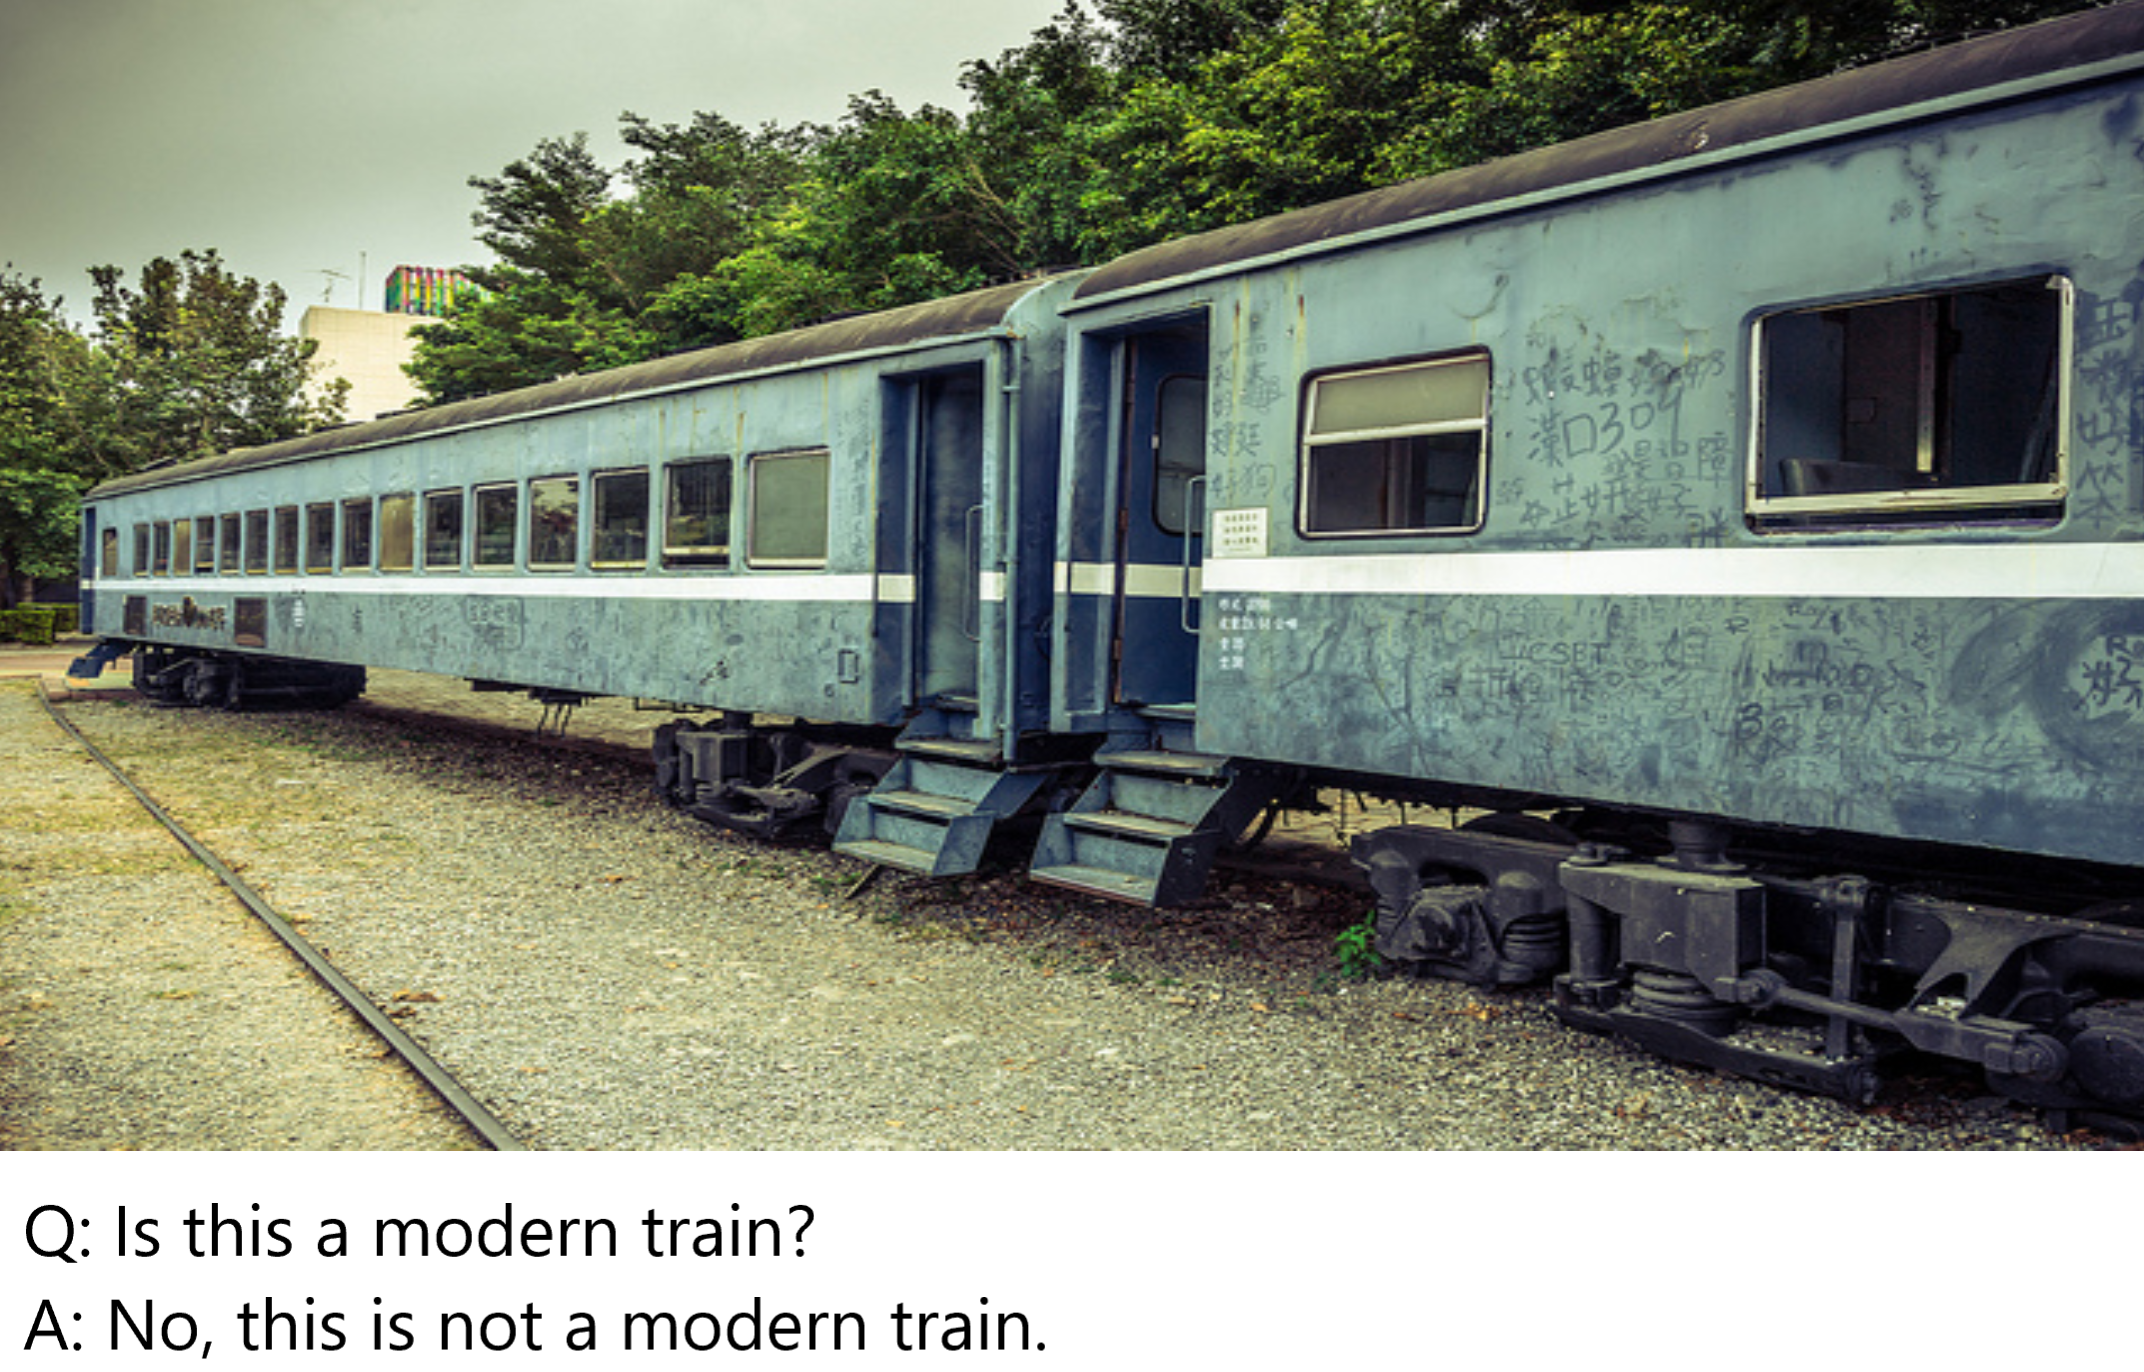
\includegraphics[width=0.7\textwidth]{figs/Intro_objective_train.png}}
    %     \caption{یک نمونه از جفت پرسش‌ و تصویر همراه با پاسخ مورد انتظار}
    %     \label{fig:intro_train}
    % \end{figure}
}
\section{ساختار گزارش}
\paragraph{}
{
    در این پروژه هدف ارائه 
    روشی نو برای حل مسئله کنترل و پایش دستگاه‌های اینترنت اشیاء بر سکوی کوبرنیتز است. 
    در ابتدا به معرفی مفاهیم پایه استفاده شده در این پروژه 
    و سپس به معرفی روش‌ها و کارهای مرتبط پرداخته‌ 
    خواهد شد. پس از آن به معرفی 
    روش و ارزیابی آن پرداخته شده است. در انتها نتیجه‌گیری و 
    کارهای آینده معرفی می‌شوند. 


}
% !TeX root=main.tex

\chapter{مفاهیم پایه} \label{ch:basics}
\thispagestyle{empty}


\section{مقدمه}
\paragraph{}
{
    در این بخش به معرفی مفاهیم پایه درباره سکوی کوبرنیتز، پروژه کوبلت مجازی، اینترنت اشیاء و برخی معماری‌هایی که 
    در این پروژه استفاده شده‌اند به مانند 
    استخر کارگران\footnote{\lr{Worker Pool}}
    پرداخته‌شده است.
}

\section{بستر ابری}
\label{sec:cloudenv}
\paragraph{}
{
    بستر ابری\footnote{\lr{Cloud Environment}}
    به محیطی اشاره دارد که منابع محاسباتی، شبکه و ذخیره سازی را برای ارائه خدمات به صورت ابری و توسط یک ارائه دهنده ابری فراهم می کند.
    در این محیط، خدمات و برنامه‌ها بر روی خدمت دهنده‌های فیزیکی مجازی‌سازی شده قرار می گیرند و کاربران می توانند به آنها از طریق اینترنت وصل شوند
    و از آنها استفاده کنند. با استفاده از محیط ابری، امکاناتی مانند انعطاف پذیری بالا، قابلیت مقیاس‌پذیری، اشتراک گذاری منابع و مدیریت
    آسانتر برای خدمات فراهم می شود. همچنین یکی از مزیت‌های بستر ابری ساده سازی ساخت، مدریت و انتشار یک خدمت می‌باشد.
}

\section{
    سکوی کوبرنیتز
}
\label{sec:kubernetes}
\paragraph{}
{
    کوبرنیتز\footnote{\lr{Kubernetes} \cite{MasteringKubernetes} \cite{44843}}
    یک سامانه مدیریت
    کانتینرها\footnote{\lr{Containers}}
    است که توسط گوگل توسعه داده شده است و در حال حاضر تحت نظارت و پشتیبانی بنیاد
    CNCF\footnote{\lr{Cloud Native Computing Foundation}}
    قرار دارد. این ابزار به توسعه‌دهندگان و مدیران سامانه امکان می‌دهد برنامه‌ها و خدمات را در
    بسترهای ابری\footnote{\lr{Cloud Environment}}
    مدیریت کنند و کانتینرها را به طور موثر و مقیاس‌پذیر در
    محیط‌های توزیع شده\footnote{\lr{Distributed Environment}}
    مدیریت کنند.
    
    از طریق کوبرنیتز، می‌توان کانتینرها را بر روی یک
    خدمت دهنده‌ مجازی\footnote{\lr{Virtual Machine}}
    یا 
    فیزیکی\footnote{\lr{Physical Server}}
    اجرا کرده و مدیریت آنها را ساده‌تر و مؤثرتر نمود. این سامانه با بهره‌گیری از روش‌هایی مانند
    اتوماسیون\footnote{\lr{automation}}
    ، توازن بار\footnote{\lr{Load Balancing}}
    و تشخیص خودکار اشکال\footnote{\lr{Automatic Diagnostics}}
    ، مدیریت و کنترل بهبود یافته‌ای در محیط‌های مبتنی بر کانتینر فراهم می‌کند.
    این ابزار برای حل مشکلات زیر موثر است:
    \begin{enumerate}
        \item مقیاس‌پذیری: کوبرنیتز می‌تواند تعداد کانتینرها و پیش‌نمونه‌های برنامه را بر اساس نیازهای ترافیک و خدمت تنظیم کند. با استفاده از مدیریت منابع مبتنی بر درخواست، میزان منابع مورد استفاده توسط برنامه را به طور خودکار تنظیم می‌کند و مقیاس‌پذیری عمودی و افقی را به راحتی فراهم می‌کند.
        \item توازن بار: با استفاده از کوبرنیتز، می‌توان بار کار را به طور متوازن بین نودها و خدمت دهنده‌های مختلف تقسیم کرد. این باعث بهبود عملکرد و عدم وقوع اختلال در سامانه می‌شود. همچنین، در صورتی که یک نود یا خدمت دهنده‌ دچار مشکل شود، کوبرنیتز به طور خودکار کار را به سایر نودها منتقل می‌کند.
        \item مدیریت پیچیدگی: کوبرنیتز امکاناتی را برای مدیریت پیچیدگی سامانه‌های کانتینری فراهم می‌کند. این ابزار اجرا، مدیریت، نظارت و زندگی‌دوباره سازی کانتینرها را ساده می‌کند. همچنین امکاناتی برای مدیریت تنظیمات، آپدیت‌ها، و تغییرات در حال اجرا نیز در اختیار کاربران قرار می‌دهد.
        \item قابلیت انتقال: کوبرنیتز امکان انتقال برنامه‌ها و خدمات بین بسترهای مختلف را فراهم می‌کند. با استفاده از این امکان، می‌توان برنامه‌ها را بین محیط‌های توسعه، آزمون و تولید به راحتی منتقل کرد. کوبرنیتز با استفاده از این قابلیت‌ها و خصوصیات، به توسعه‌دهندگان و مدیران سامانه امکان می‌دهد برنامه‌ها را به صورت مؤثر، قابلیت مقیاس‌پذیری و قابل اطمینان در محیط‌های کانتینری مدیریت کنند و عملکرد سامانه را بهبود دهند.
    \end{enumerate}
    \begin{figure}[H]
        \center{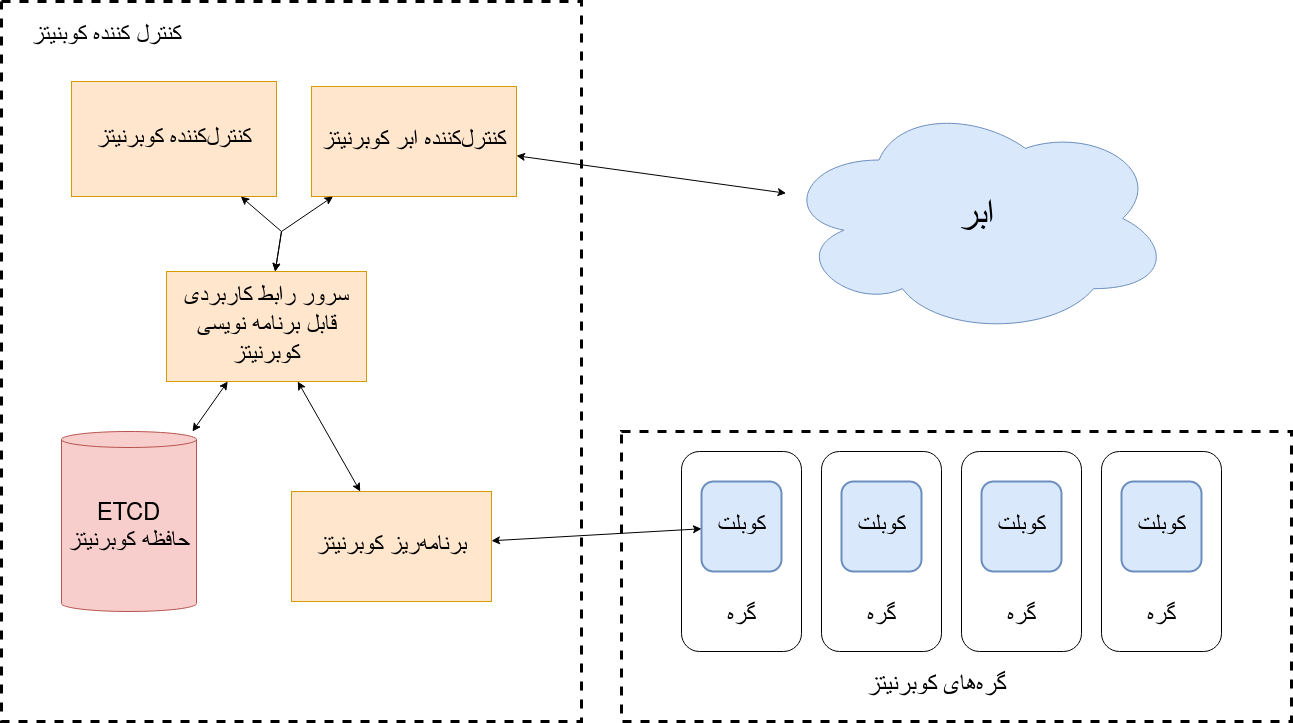
\includegraphics[width=\textwidth]{figs/kube_compontents.png}}
        \caption{معماری کلی کوبرنیتز}
        \label{fig:kube_compontents}
    \end{figure}
}

\subsection{کانتینر‌}
\label{subsec:containers}
\paragraph{}
{
    کانتینرها یک فناوری پیشرفته در زمینه مدیریت و اجرای نرم‌افزار هستند. یک کانتینر، یک واحد نرم‌افزاری است که تمام نیازمندی‌های
    لازم برای اجرای یک نرم‌افزار را شامل می‌شود. در واقع، کانتینرها مجموعه‌ای از عملیات سامانه‌ای، کدها و تنظیماتی هستند که با 
    یکدیگر در یک بستر محصور می‌شوند. از ویژگی‌های برجسته کانتینرها، می‌توان به استقلال و حمل‌پذیری آن‌ها اشاره کرد. به عبارتی دیگر،
    یک کانتینر می‌تواند بدون تغییر و با حفظ کارایی خود، بین بستر‌ها و سامانه‌‌های عامل‌ منتقل شود. این ویژگی باعث شده است که کانتینرها
    در صنعت فناوری اطلاعات بسیار محبوب شوند. برای مدیریت کانتینرها، ابزارهای مختلفی وجود دارند. یکی از محبوب‌ترین ابزارها برای مدیریت کانتینرها،
    داکر\footnote{\lr{Docker} \cite{7912109}}
    است. داکر یک بستر توسعه نرم‌افزار مبتنی بر کانتینر است که به توسعه‌دهندگان امکان می‌دهد تا برنامه‌های خود را در یک کانتینر قرار داده و آن را در
    هر سامانه‌ای اجرا کنند. با استفاده از کانتینرها، عملیات توسعه، آزمون و استقرار نرم‌افزارها سریع‌تر و ساده‌تر می‌شود. با توجه به این که هر کانتینر
    دارای محیط مستقلی است، احتمال بروز تداخل بین برنامه‌ها به حداقل می‌رسد و تغییرات در یک کانتینر بر روی سایر کانتینرها تأثیری نمی‌گذارد. همچنین،
    سبک بودن کانتینرها امکان مقیاس‌پذیری بالایی را فراهم می‌آورد.
}

\subsection{پاد}
\label{subsec:pod}
\paragraph{}
{
    پاد‌ها\footnote{\lr{Pods}} در کوبنیتز واحد اصلی اجرا و مدیریت برنامه‌ها و خدمات هستند. یک پاد شامل یک یا چند کانتینر مرتبط است که به صورت مشترک منابع شبکه و ذخیره‌سازی را به اشتراک می‌گذارند. همچنین، هر پاد دارای یک آدرس یکتا درون کلاستر است. پاد‌ها به صورت لایه‌ای مجازی شبیه سازی می‌شوند و انتزاعی از یک    مجازی یا سیستم‌عامل فیزیکی هستند. این انتزاع به برنامه‌ها امکان می‌دهد تا بدون احتیاج به اطلاعات جزئیات بستری که برای اون اجرا می‌شوند، در محیط کنترلی کوبرنیتز اجرا شوند. بنابراین، پاد‌ها برای توسعه‌دهندگان و مدیران سامانه، یک واسط سطح بالا و یک فضای کاری است.
}

\subsection{گره}
\label{subsec:node}
\paragraph{}
{
    در بستر کوبنیتز، گره‌ها\footnote{\lr{Node}} از اجزای کلیدی هستند که برنامه‌ها و خدمات در آن‌ها اجرا می‌شوند. یک گره 
    معمولاً یک خدمت دهنده‌ فیزیکی یا ماشین مجازی است که بر روی آن کانتینرها اجرا می‌شوند. هر گره شامل عناصر زیر است:
    \begin{enumerate}
        \item پلتفرم سخت‌افزاری: این شامل خدمت دهنده‌ها، سامانه‌های فیزیکی، یا ماشین‌های مجازی است که منابع سخت‌افزاری مانند پردازنده، حافظه، و دیسک را فراهم می‌کنند. گره‌ها بسته به نیازهای برنامه‌ها و خدمات، می‌توانند از طریق شبکه به یکدیگر متصل شوند.
        \item کوبلت\footnote{\lr{Kublet}}: مسئول مدیریت و اجرای کانتینرها در گره است. آن بر روی هر گره نصب شده و با کنترل کننده‌های کوبرنیتز برای دریافت توصیف کانتینرها و مدیریت آن‌ها در ارتباط است.
        \item پروکسی\footnote{\lr{Kube-proxy}}: یک کنترل کننده شبکه است که مسئول مدیریت ترافیک شبکه بین کانتینرها در گره است. این عملکرد به ارتباط و مسیریابی درخواست‌ها بین کانتینرها و اجزای دیگر کوبرنیتز مرتبط است.
        \item حافظه مشترک\footnote{\lr{Shared Memory}}: گره‌ها از یک حافظه مشترک برای ذخیره و به اشتراک گذاری اطلاعاتی مانند پیکربندی‌ها و وضعیت گره‌ها استفاده می‌کنند. این حافظه مشترک معمولاً از طریق ابزارهای ذخیره‌سازی مانند ETCD پیاده‌سازی می‌شود.
    \end{enumerate}
    با استفاده از گره‌ها، کوبرنیتز قادر است برنامه‌ها و خدمات را بر روی یک سری از خدمت دهنده‌ها یا ماشین‌های مجازی توزیع کند و به طور همزمان و مقیاس‌پذیر اجرا کند. این باعث افزایش انعطاف‌پذیری، بهره‌وری و پایداری در محیط‌های ابری و مجازی می‌شود.
}

\subsection{کوبلت}
\label{subsec:kubelet}
\paragraph{}
{
    کوبلت
    یکی از اجزای اصلی سامانه مدیریت کانتینرها کوبرنیتز است. کوبلت مسئول اجرا و مدیریت کانتینرها در یک
    گره
    می‌باشد. کوبلت در هر گره از
    خوشه\footnote{\lr{Cluster}}
    کوبرنیتز نصب شده و وظیفه‌ای اساسی را بر عهده دارد که شامل موارد زیر است:
    \begin{enumerate}
        \item مدیریت کانتینرها: کوبلت مسئول ساخت و اجرای کانتینرها بر اساس توصیف‌هایی که از طرف کنترل کننده‌های کوبرنیتز به آن ارسال می‌شود، می‌باشد. این توصیف‌ها شامل اطلاعاتی مانند نرم‌افزار مورد نظر، تنظیمات شبکه و منابع مصرفی کانتینر می‌شوند.
        \item پایش\footnote{\lr{Monitoring}}منابع: کوبلت مسئول نظارت بر منابع مصرفی کانتینرها است و اطلاعات مربوط به استفاده از پردازنده، حافظه، شبکه و دیگر منابع سامانه را جمع‌آوری کرده و گزارش می‌دهد. این اطلاعات به کنترل کننده‌های کوبرنیتز ارسال می‌شوند تا بتوانند به‌طور هوشمند منابع را تخصیص دهند و بهینه‌سازی منابع را انجام دهند.
        \item بروزرسانی و نگهداری کانتینرها: کوبلت مسئول بروزرسانی و نگهداری کانتینرها است. اگر نسخه جدیدی از نرم‌افزار موجود باشد، کوبلت قادر است آن را دریافت و کانتینرها را بروزرسانی کند. همچنین، در صورت خطا در اجرای کانتینر یا توقف آن، کوبلت تلاش می‌کند کانتینر را به‌طور خودکار مجدداً راه‌اندازی کند.
        \item ارتباط با سایر اجزا: کوبلت وظیفه برقراری ارتباط با اجزای دیگر کوبرنیتز را نیز دارد. به‌عنوان مثال، با کنترل کننده\footnote{\lr{kube-controller-manager}} برای دریافت دستورات مدیریتی، با برنامه‌ریز\footnote{\lr{kube-scheduler}} برای دریافت جدول‌بندی پیشنهادی و با کنترل کننده شبکه\footnote{\lr{kube-proxy}} برای تنظیمات شبکه در ارتباط است.
    \end{enumerate}
    به طور خلاصه، کوبلت یکی از اجزای کلیدی کوبرنیتز است که وظیفه مدیریت و اجرای کانتینرها را در گره‌های سامانه بر عهده دارد. این کامپوننت از طریق ارتباط با سایر اجزا و دریافت توصیف‌های مربوطه، به ایجاد و مدیریت یک محیط توزیع شده و مقیاس‌پذیر برای اجرای برنامه‌ها و خدمات در کوبرنیتز کمک می‌کند.
}

\subsection{خوشه کوبرنیتز}
\label{subsec:kube_cluster}
\paragraph{}
{
    یک خوشه کوبنیتز\footnote{\lr{Kubernetes Cluster}} یک بستر توزیع شده است که شامل مجموعه‌ای از گره‌ها است که برای مدیریت و اجرای برنامه‌ها و ارائه خدمات از طریق کوبنیتز استفاده می‌شود. خوشه کوبنیتز شامل اجزا و خدماتی متعددی است که با همکاری میان گره‌ها، برنامه‌ها را مدیریت می‌کنند.
}

\section{قرارداد انتقال فرا متن}
\label{sec:http}
\paragraph{}
{
    قرارداد انتقال فرا متن\footnote{\lr{Hypertext Transfer Protocol (HTTP)}} یک پروتکل ارتباطی است که در اینترنت استفاده می‌شود و برای انتقال اطلاعات بین خدمت دهنده‌\footnote{\lr{Server}} و خدمت گیرنده\footnote{\lr{Client}} استفاده می‌شود. به طور کلی، قرارداد انتقال فرا متن به عنوان روشی برای انتقال اطلاعات و محتوا در وب مورد استفاده قرار می‌گیرد. در یک ارتباط HTTP، خدمت گیرنده درخواستی به خدمت دهنده‌ می‌فرستد و سپس خدمت دهنده‌ با پاسخ مناسب به درخواست خدمت گیرنده پاسخ می‌دهد. این درخواست و پاسخ در قالب پیام‌های متنی انجام می‌شود، که ممکن است شامل سرآیندها\footnote{\lr{Header}} و محتوای پیام\footnote{\lr{Body}} باشند. سرآیندها شامل اطلاعاتی مانند نوع محتوا، تاریخ، طول پیام و سایر جزئیات مربوط به ارتباط است. قرارداد انتقال فرا متن برای انتقال انواع مختلف منابع و اطلاعات در وب استفاده می‌شود. مثلاً می‌توان از قرارداد انتقال فرا متن برای دریافت صفحات وب، تصاویر، ویدیوها و سایر منابع در خدمت دهنده‌ استفاده کرد. همچنین، قرارداد انتقال فرا متن از مدل درخواست-پاسخ پیروی می‌کند، به این معنی که خدمت گیرنده درخواستی ارسال می‌کند و خدمت دهنده‌ با یک پاسخ مناسب به آن پاسخ می‌دهد. قرارداد انتقال فرا متن اساسی است در عملکرد وب و تعامل بین سرویس‌دهنده و خدمت گیرنده. این پروتکل به صورت گسترده در نرم‌افزارها و سرویس‌های وب مورد استفاده قرار می‌گیرد و امکان انتقال اطلاعات و ارتباط بین کامپیوترها و دستگاه‌ها را فراهم می‌کند.
    \begin{figure}[H]
        \center{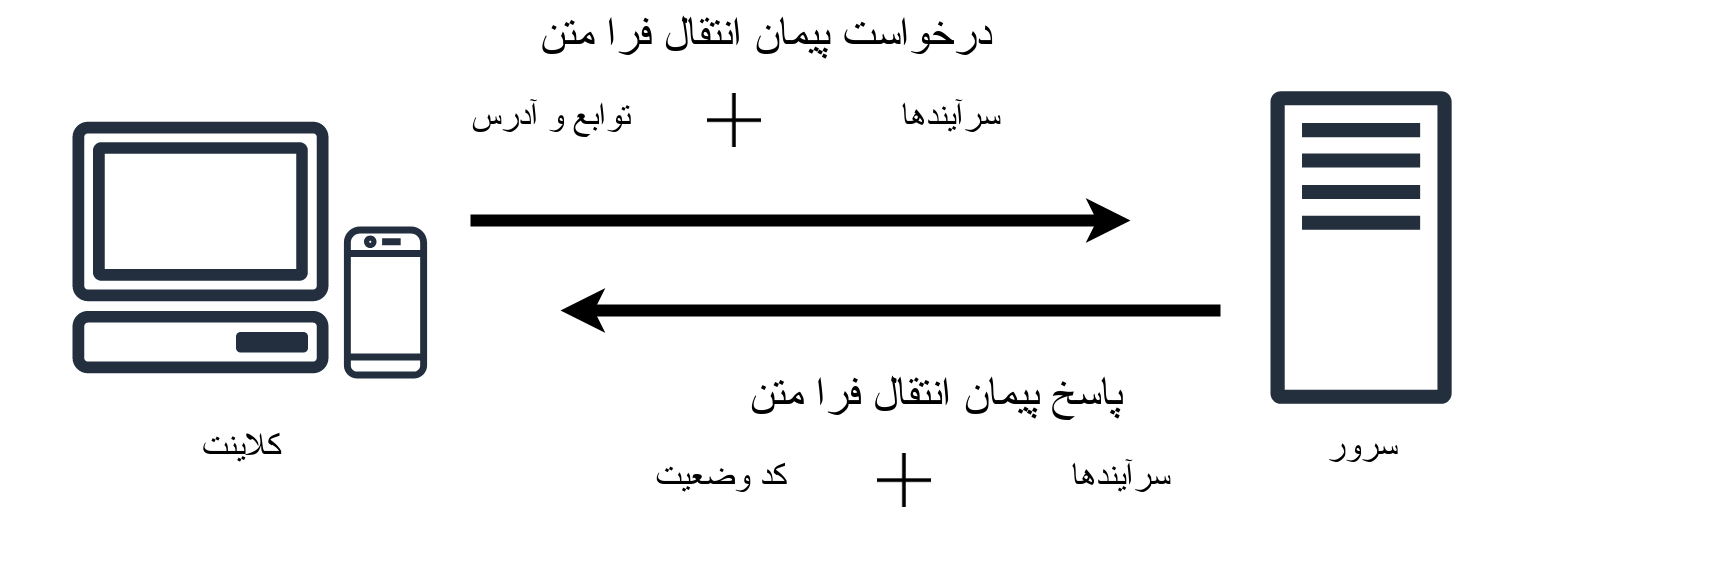
\includegraphics[width=\textwidth]{figs/http.png}}
        \caption{نمای کلی درخواست و پاسخ قرارداد انتقال فرا متن}
        \label{fig:http}
    \end{figure}
}

\subsection{توابع قرارداد انتقال فرا متن}
\label{subsec:http_methods}
\paragraph{}
{
    قرارداد انتقال فرا متن توابع\footnote{\lr{قرارداد انتقال فرا متن Methods}} مختلفی را برای تعیین نوع عملیاتی که باید انجام شود تعریف کرده است که عبارت است از:
    \begin{enumerate}
        \item دریافت\footnote{\lr{GET}}: این تابع برای دریافت (خواندن) اطلاعات از یک منبع مشخص درخواست می‌شود. مثلاً با استفاده از تابع دریافت می‌توانید صفحات وب، تصاویر یا سایر منابع را از خدمت دهنده‌ دریافت کنید. درخواست دریافت، بدون تغییر و اثری روی منبع مورد درخواست، انجام می‌شود.
        \item ساخت\footnote{\lr{POST}}: این تابع برای ارسال داده‌ها به خدمت دهنده‌ استفاده می‌شود. از تابع ساخت برای ایجاد یا ارسال داده جدید به خدمت دهنده‌ استفاده می‌شود، مانند ارسال فرم‌ها در وب، ارسال نظرات یا انجام عملیات‌های پردازشی. درخواست ساخت می‌تواند تغییراتی روی منبع مورد درخواست ایجاد کند.
        \item بروزرسانی\footnote{\lr{PUT}}: این تابع برای به‌روزرسانی (بازنویسی) یک منبع مشخص استفاده می‌شود. با استفاده از تابع بروزرسانی، می‌توانید اطلاعات موجود در خدمت دهنده‌ را با داده‌های جدید جایگزین کنید. درخواست بروزرسانی می‌تواند تغییراتی روی منبع مورد درخواست اعمال کند یا در صورت عدم وجود، یک منبع جدید ایجاد کند.
        \item حذف\footnote{\lr{DELETE}}: این تابع برای حذف یک منبع مشخص استفاده می‌شود. با استفاده از تابع حذف می‌توانید یک منبع را از خدمت دهنده‌ حذف کنید. درخواست حذف، منبع مورد نظر را از خدمت دهنده‌ حذف می‌کند.
        \item بروزرسانی مقطعی\footnote{\lr{PATCH}}: این تابع برای اعمال تغییرات جزئی روی یک منبع مشخص استفاده می‌شود. با استفاده از تابع بروزرسانی مقطعی، می‌توانید تغییرات کوچکی را روی یک منبع اعمال کنید بدون ایجاد تغییرات بزرگتری در داده‌های موجود.
    \end{enumerate}
    این توابع به عنوان پایه‌های قرارداد انتقال فرا متن عمل می‌کنند و به خدمت گیرنده و خدمت دهنده‌ امکان ارتباط و انجام عملیات‌های مختلف را می‌دهند. درخواست‌ها و پاسخ‌های قرارداد انتقال فرا متن بر اساس این توابع تعریف می‌شوند و برای تعامل موثر بین سرویس‌دهنده و خدمت گیرنده استفاده می‌شوند.
}

\subsection{درخواست قرارداد انتقال فرا متن}
\label{subsec:http_requests}
\paragraph{}
{
    در قرارداد انتقال فرا متن، وقتی که خدمت گیرنده (مانند مرورگر وب یا برنامه‌ای که درخواست ارسال می‌کند) برای دستیابی به منبع مورد نظر خود، درخواستی\footnote{\lr{HTTP Request}} ایجاد می‌کند، یک درخواست قرارداد انتقال فرا متن ایجاد می‌شود. درخواست‌های قرارداد انتقال فرا متن شامل اطلاعاتی درباره نوع و منبع درخواست شده هستند. در زیر توضیحی از مهمترین اجزای یک درخواست قرارداد انتقال فرا متن را می‌یابید:
    \begin{enumerate}
        \item توابع قرارداد انتقال فرا متن: تابع مشخص می‌کند خدمت گیرنده درخواست انجام چه عملیاتی را بر روی منبع مورد نظر دارد.
        \item درس\footnote{\lr{Uniform Resource Locator (URL)}}: مشخص می‌کند که منبع مورد نظر کجا قرار دارد و آدرس دقیق آن چیست. آدرس شامل پروتکل، نام دامنه خدمت دهنده‌\footnote{\lr{Domain Name}} و مسیر\footnote{\lr{Path}} منبع مورد نظر است.
        \item سرآیندها: درخواست قرارداد انتقال فرا متن می‌تواند شامل سرآیندها باشد که اطلاعات اضافی درباره درخواست و مشخصات خدمت گیرنده را ارائه می‌دهند. به عنوان مثال، سرآیندها می‌توانند شامل اطلاعات مربوط به نوع محتوا، زبان مورد نظر، تاریخ و غیره باشند.
        \item بدنه درخواست\footnote{\lr{Request Body}}: بدنه درخواست، در صورتی که درخواست ارسالی دارای داده‌های ارسالی است، این داده‌ها را در خود نگه می‌دارد. بدنه درخواست به صورت متنی یا در قالب داده‌های باینری می‌تواند باشد و معمولاً در درخواست‌هایی مانند ساخت و بروزرسانی استفاده می‌شود.
    \end{enumerate}
    هنگامی که خدمت گیرنده درخواست قرارداد انتقال فرا متن را به خدمت دهنده‌ ارسال می‌کند، خدمت دهنده‌ با استفاده از اطلاعات درخواست، منبع مورد نظر را پیدا کرده و به مناسبت درخواست، پاسخ مناسب را به خدمت گیرنده ارسال می‌کند. درخواست‌های قرارداد انتقال فرا متن بسته به نوع و عملیات مورد نظر، تعیین می‌کنند که چه عملیاتی باید در سمت خدمت دهنده‌ انجام شود و اطلاعات مربوطه را برگردانند.
}

\subsection{پاسخ‌ قرارداد انتقال فرا متن}
\label{subsec:http_responses}
\paragraph{}
{
    هنگامی که یک درخواست از سوی خدمت گیرنده به خدمت دهنده‌ ارسال می‌شود، خدمت دهنده‌ با یک پاسخ\footnote{\lr{HTTP Response}} مناسب به آن درخواست پاسخ می‌دهد. پاسخ‌های قرارداد انتقال فرا متن حاوی اطلاعات مربوط به نتیجه درخواست و وضعیت آن است.
    \begin{enumerate}
        \item کد وضعیت\footnote{\lr{Status Code}}: هر پاسخ قرارداد انتقال فرا متن دارای یک کد وضعیت است که نشان می‌دهد درخواست با موفقیت انجام شده است یا با مشکل مواجه شده است. برخی از کدهای وضعیت رایج عبارتند از:
            \begin{table}[h]
                \begin{tabular}{|c|c|}
                \hline
                کد پاسخ & شرح                                                                                  \\ \hline
                ۲۰۰     & درخواست ﺑﺎ ﻣﻮﻓﻘﯿﺖ اﻧﺠﺎم ﺷﺪه اﺳﺖ و پاسخ داده ﻣﻮرد ﻧﻈﺮ در دﺳﺘﺮس اﺳﺖ                     \\ \hline
                ۲۰۱     & منبع مورد نظر با موفقیت ساخته شد                     \\ \hline
                ۲۰۴     & پاسخ بدون بدنه                     \\ \hline
                ۴۰۴     & ﻣﻨﺒﻊ ﻣﻮرد ﻧﻈﺮ پیدا ﻧﺸﺪ                                                               \\ \hline
                ۵۰۰     & مشکلی در ﺳﻤﺖ ﺧﺪﻣﺖ دﻫﻨﺪه رخ داده اﺳﺖ که ﻣﻮﺟﺐ ﻋﺪم ﺗﻮاﻧﺎﯾی در ارﺳﺎل پاسخ ﻣﻮرد ﻧﻈﺮﺷﺪه اﺳﺖ \\ \hline
                \end{tabular}
                \caption{جدول کد پاسخ‌های متداول قرارداد انتقال فرا متن}
                \label{http_status_codes_table}
            \end{table}
            \\
        \item سرآیندها: پاسخ قرارداد انتقال فرا متن شامل سرآیندها است که اطلاعات اضافی در مورد پاسخ و منبع مورد نظر را ارائه می‌دهند. به عنوان مثال، سرآیندها می‌توانند شامل اطلاعات مربوط به نوع محتوا، طول پاسخ، تاریخ ارسال، و غیره باشند.
        \item محتوای پاسخ\footnote{\lr{Response Body}}: پاسخ قرارداد انتقال فرا متن ممکن است حاوی محتوای مورد نظر باشد که توسط خدمت دهنده‌ ارسال می‌شود. محتوای پاسخ می‌تواند اطلاعاتی مانند متن، تصویر، ویدیو یا سایر منابع مورد نیاز را شامل شود.
    \end{enumerate}
    پاسخ‌های قرارداد انتقال فرا متن ارسال شده توسط خدمت دهنده‌ معمولاً به درخواست‌های ارسالی از سوی مشتری پاسخ می‌دهند و اطلاعات مورد نیاز را در اختیار مشتری قرار می‌دهند. این پاسخ‌ها با کدهای وضعیت، سرآیندها و محتوای پاسخ کامل شده و تعیین می‌کنند که درخواست با موفقیت انجام شده است یا خطا رخ داده است.
}

\subsection{انتقال حالت نمایشی}
\label{subsec:rest}
\paragraph{}
{
    انتقال حالت نمایشی\footnote{\lr{Representational State Transfer (REST)}} یک معماری نرم‌افزاری است که برای طراحی سامنه‌های توزیع‌شده و مبتنی بر وب استفاده می‌شود. انتقال حالت نمایشی بر اساس مجموعه‌ای از اصول و محدودیت‌ها ساختاردهی شده است که در تبادل اطلاعات بین خدمت دهنده‌ و خدمت گیرنده نقش مهمی دارد. یکی از اصول اساسی انتقال حالت نمایشی، تعریف یکپارچگی\footnote{\lr{Uniform Interface}} برای سامنه است. این به این معنی است که سامنه باید یک مجموعه‌ی مشخص از روش‌های استاندارد را برای تعاملات در نظر بگیرد. معمولاً در سامنه‌های انتقال حالت نمایشی، از متدهای قرارداد انتقال فرا متن مانند دریافت، ساخت، بروزرسانی و حذف برای تعیین عملیات مورد نیاز استفاده می‌شود. همچنین، منابع\footnote{\lr{Resources}} در سامنه انتقال حالت نمایشی به صورت یکتا شناسایی می‌شوند و آدرس‌های مشخصی برای آنها تعیین می‌شود.با توجه به این اصول و محدودیت‌ها، سامنه‌های انتقال حالت نمایشی قابلیت‌هایی مانند قابلیت توزیع، قابلیت مقیاس‌پذیری، انعطاف‌پذیری و قابلیت استفاده مجدد را فراهم می‌کنند. از طریق روش‌های استاندارد و اصول انتقال حالت نمایشی، سامنه‌ها قادر به تعامل با یکدیگر بدون توجه به جزئیات داخلی و پیچیدگی‌های نحوه پیاده‌سازی هستند.   
    \begin{figure}[H]
        \center{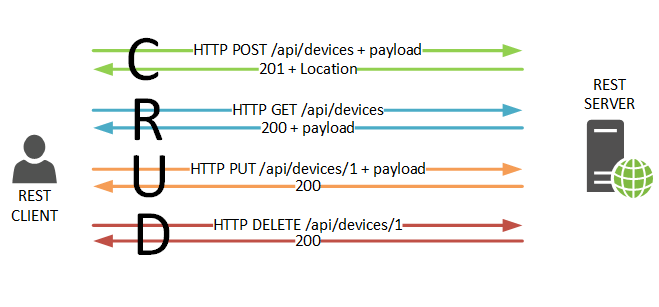
\includegraphics[width=\textwidth]{figs/rest-crud.png}}
        \caption{نمای کلی از انتقال حالت نمایشی}
        \label{fig:rest}
    \end{figure}
}

\subsection{رابط کاربردی قابل برنامه‌ریزی}
\label{subsecsec:api}
\paragraph{}
{
    رابط کاربردی قابل برنامه‌ریزی\footnote{\lr{Application Programming Interface}} به قوانین، پروتکل‌ها و دستوراتی گفته می‌شود که برای ارتباط و 
    تعامل بین نرم‌افزارها، خدمات و برنامه‌های مختلف به کار می‌رود. به طور کلی، رابط کاربردی قابل برنامه‌ریزی نقش یک میانجی بین سامانه‌ها را بازی
    می‌کند و به برنامه‌نویسان اجازه می‌دهد با استفاده از آن، به منابع و امکانات موجود در سامانه دیگر دسترسی پیدا کنند. رابط کاربردی قابل برنامه‌ریزی‌ها
    می‌توانند در دو شکل مختلف عمل کنند: به صورت وب خدمت یا به صورت کتابخانه برنامه‌نویسی. در حالت وب خدمت، رابط کاربردی قابل برنامه‌ریزی بر روی
    یک خدمت دهنده‌ میزبان شده است و از طریق پروتکل‌های اینترنتی مانند قرارداد انتقال فرا متن قابل دسترسی است. در حالت کتابخانه برنامه‌نویسی، دستورات و توابع مشخصی به
    برنامه اضافه می‌شوند که برنامه‌نویسان می‌توانند از آنها به عنوان قسمتی از برنامه خود استفاده کنند. استفاده از رابط کاربردی قابل برنامه‌ریزی‌ها
    به برنامه‌نویسان امکان می‌دهد که بخشی از دستورات را استفاده کنند و از خدمات و قابلیت‌های ارائه شده توسط یک سامانه دیگر بهره ببرند. این 
    راهکار می‌تواند زمان و هزینه توسعه برنامه را کاهش داده و امکان ادغام بین نرم‌افزارها را فراهم کند. به طور خلاصه، رابط کاربردی قابل برنامه‌ریزی
    .مانند یک پل ارتباطی است که برنامه‌نویسان می‌توانند از آن استفاده کنند تا بین نرم‌افزارها و خدمات اطلاعات را به اشتراک بگذارند و تعامل کنند.
    \begin{figure}[H]
        \center{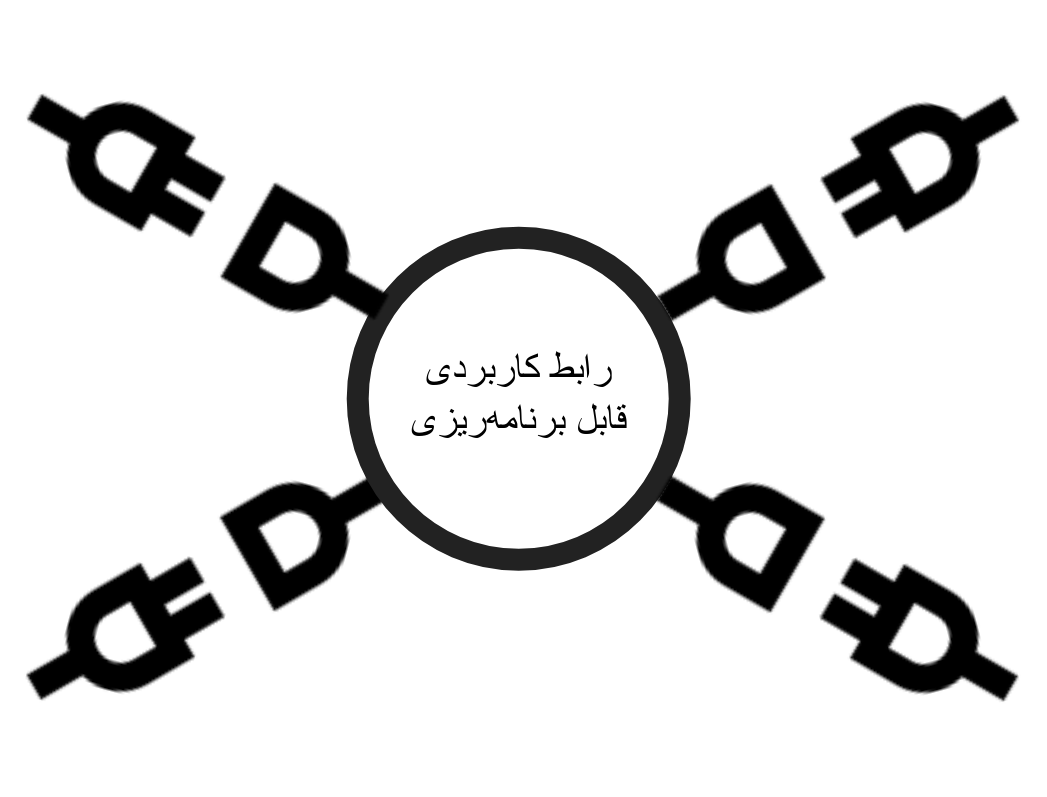
\includegraphics[width=\textwidth]{figs/api.png}}
        \caption{نمای کلی از رابط کاربردی قابل برنامه‌ریزی}
        \label{fig:api}
    \end{figure}
}

\section{معماری Fan-Out}
\label{sec:fanout}
\paragraph{}
{
    معماری Fan-Out: الگوی طراحی است که به طور معمول در سامانه‌های توزیع‌شده برای مدیریت همزمان یا موازی درخواست‌ها استفاده می‌شود. این معماری به توزیع درخواست‌های ورودی به چند واحد پردازش ، که به عنوان کارگرها شناخته می‌شوند، برای انجام عملیات مورد نیاز می‌پردازد. معماری Fan-Out با بهره‌گیری از پردازش موازی و توازن بار، امکان مقیاس‌پذیری و بهبود عملکرد سیستم را فراهم می‌کند. در معماری Fan-Out، هنگامی که یک درخواست دریافت می‌شود، آن را به چندین کارگر مستقل تکرار یا ارسال می‌کنند تا هر کدام از آن‌ها قادر به پردازش درخواست به صورت مستقل باشند. این رویکرد به چندین کارگر اجازه می‌دهد تا به صورت همزمان روی بخش‌های مختلف درخواست کار کنند و بهبود ظرفیت تولید و کاهش زمان پاسخ را به همراه داشته باشد.
    \begin{figure}[H]
        \center{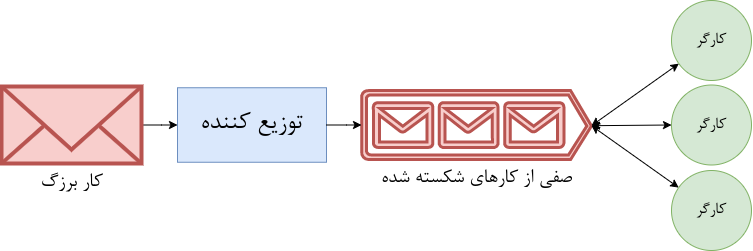
\includegraphics[width=\textwidth]{figs/fanout.png}}
        \caption{نمای کلی از معماری Fan-Out}
        \label{fig:fanout}
    \end{figure}
}

\section{کوبلت مجازی}
\label{sec:vritkubelet}
\paragraph{}
{
    کوبلت مجازی\footnote{\lr{Virtual Kubelet} \cite{VIRTUALKUBELET}} یک پروژه متن باز است که با گسترش رابط‌ کاربردی قابل برنامه‌ریزی کوبرنیتز، امکان ادغام\footnote{\lr{Integration}} خدمات و سامانه‌های خارجی را در قالب گره‌های کوبرنیتز فراهم می‌کند. این پروژه این امکان را می‌دهد که یک گره "مجازی" بسازیم که توسط کوبرنیتز قابل مدیریت باشد و امکان ادغام سامانه‌های متنوع را در داخل خوشه کوبرنیتز به صورت یک‌پارچه فراهم کند.    
    \begin{figure}[H]
     \center{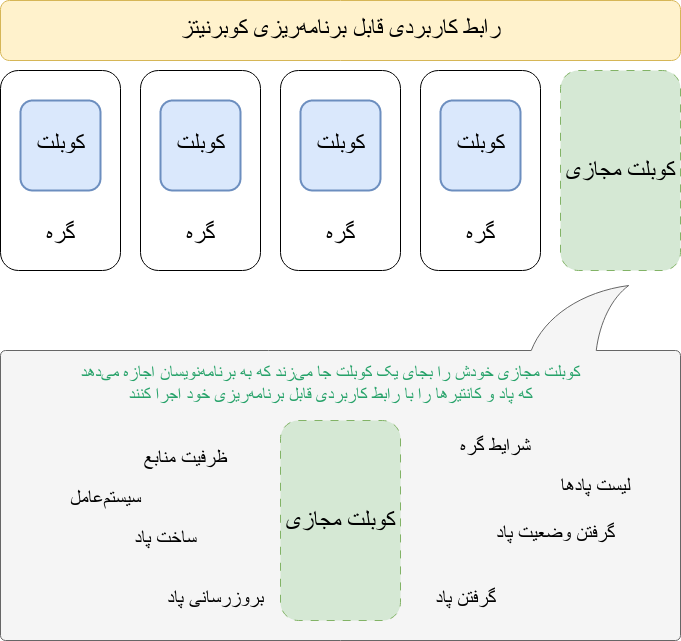
\includegraphics[width=0.8\textwidth]{figs/vkube.png}}
     \caption{کوبلت مجازی در یک خوشه کوبرنیتز}
     \label{fig:virtkublet_arch}vkube
    \end{figure}
}

\subsection{معماری کوبلت مجازی}
\label{subsec:vkube_arch}
\paragraph{}
{
    کوبلت مجازی از چندین بخش کلیدی تشکیل شده است:
    \begin{enumerate}
        \item تامین‌کننده: تامین‌کننده مسئول پیاده‌سازی رابط کوبلت مجازی است و به عنوان پل ارتباطی بین سامانه یا خدمت خارجی و کوبرنیتز عمل می‌کند. این بخش، فراخوانی‌های رابط کاربردی قابل برنامه‌ریزی کوبرنیتز را به عملیات مناسب در سامانه خارجی ترجمه می‌کند.
        \item گره: گره مجازی نمایانگر یک سامانه یا خدمت خارجی در خوشه کوبرنیتز است. عملکرد آن شبیه یک گره کوبرنیتز عادی است، اما به جای اجرا در زیرساخت فیزیکی، از طریق تامین‌کننده با سامانه خارجی ارتباط برقرار می‌کند.
        \item پاد: پاد در کوبرنیتز، شامل یک یا چند کانتینر است. در کوبلت مجازی، پادها نماینده کارها\footnote{\lr{Workload}} هستند که در گره‌های مجازی ایجاد شده توسط سامانه خارجی اجرا می‌شوند.
        \item برنامه‌ریز\footnote{\lr{Scheduler}}: برنامه‌ریز کوبرنیتز مسئول تخصیص پادها به گره‌های موجود بر اساس نیازهای منابع و محدودیت‌ها است. در کوبلت مجازی، برنامه‌ریز مسئول زمانبندی پادها به گره‌های مجازی ایجاد شده توسط تامین‌کننده است. این بخش تضمین می‌کند که منابع بصورت بهینه استفاده شده و کارها به طور مناسب در سامانه خارجی توزیع شوند.
    \end{enumerate}
}

\section{اینترنت اشیاء}
\label{sec:iot}
\paragraph{}
{   
    اینترنت اشیاء\footnote{\lr{Internt of Things (IoT)}} به مجموعه‌ای از دستگاه‌ها، سنسورها، دستگاه‌های هوشمند و شبکه‌های مرتبط که قادر
    به تبادل اطلاعات با یکدیگر از طریق اتصال به اینترنت هستند، اشاره دارد. این اشیاء می‌توانند شامل تلفن همراه‌ها و ساعت هوشمند تا لوازم
    خانگی هوشمند، خودروهای متصل و تجهیزات صنعتی باشند. اینترنت اشیاء با اتصال اشیاء و جمع‌آوری اطلاعات، امکان برقراری ارتباط و کنترل 
    بیشتری را بین دنیای فیزیکی و دنیای دیجیتال فراهم می‌کند. مزیت اصلی اینرنت اشیاء در جمع‌آوری و تبادل داده‌ها است. سنسورها و دستگاه‌ها 
    در اینترنت اشیاء می‌توانند اطلاعات مربوط به بستر، شرایط، موقعیت جغرافیایی، وضعیت و داده‌های دیگر را جمع‌آوری کرده و به خدمت دهنده‌ها یا سامانه‌های 
    مرکزی ارسال کنند. این اطلاعات در خدمت دهنده‌ها تحلیل می‌شوند و می‌توانند به عنوان منبعی برای ارائه داده‌های مفید، تجزیه و تحلیل ترافیک، پیش‌بینی و 
    اتخاذ تصمیم‌های هوشمند استفاده شوند. از جمله کاربردهای اینترنت اشیاء می‌توان به موارد زیر اشاره کرد:
    \begin{enumerate}
        \item خانه هوشمند: اتصال لوازم خانگی مانند تلویزیون، سامانه‌های روشنایی، دستگاه‌های گرمایشی و سرمایشی، سامانه‌های امنیتی و سایر دستگاه‌ها به اینترنت به کاربران امکان می‌دهد تا این دستگاه‌ها را از راه دور کنترل و مدیریت کنند.
        \item صنعت هوشمند: در صنعت، اینترنت اشیاء می‌تواند در جمع‌آوری داده‌ها از تجهیزات و سنسورها به منظور نظارت بر فرآیندها، پیشگیری از خرابی‌ها، بهینه‌سازی استفاده از منابع و افزایش بهره‌وری مورد استفاده قرار گیرد.
        \item شهر هوشمند: با استفاده از سنسورها و دستگاه‌های اینترنت اشیاء، می‌توان شهرها را هوشمندتر کرده و بهبود امکانات شهری مانند مدیریت ترافیک، پارکینگ هوشمند، مدیریت پسماند و رصد آلودگی هوا را فراهم کرد.
        \item سلامتی هوشمند: استفاده از دستگاه‌های پوشیدنی، سنسورها و دستگاه‌های پزشکی هوشمند، امکان نظارت بر سلامتی فرد، جمع‌آوری داده‌های پزشکی، پیشگیری از بیماری‌ها و ارائه مراقبت بهتر را فراهم می‌کند.
    \end{enumerate}
    به طور کلی، اینترنت اشیاء با اتصال اشیاء به اینترنت و جمع‌آوری داده‌ها، امکانات جدیدی را در دسترس قرار می‌دهد و قابلیت های جدیدی را برای کنترل، مدیریت و بهبود عملکرد اشیا فراهم می‌کند.
    \begin{figure}[H]
        \center{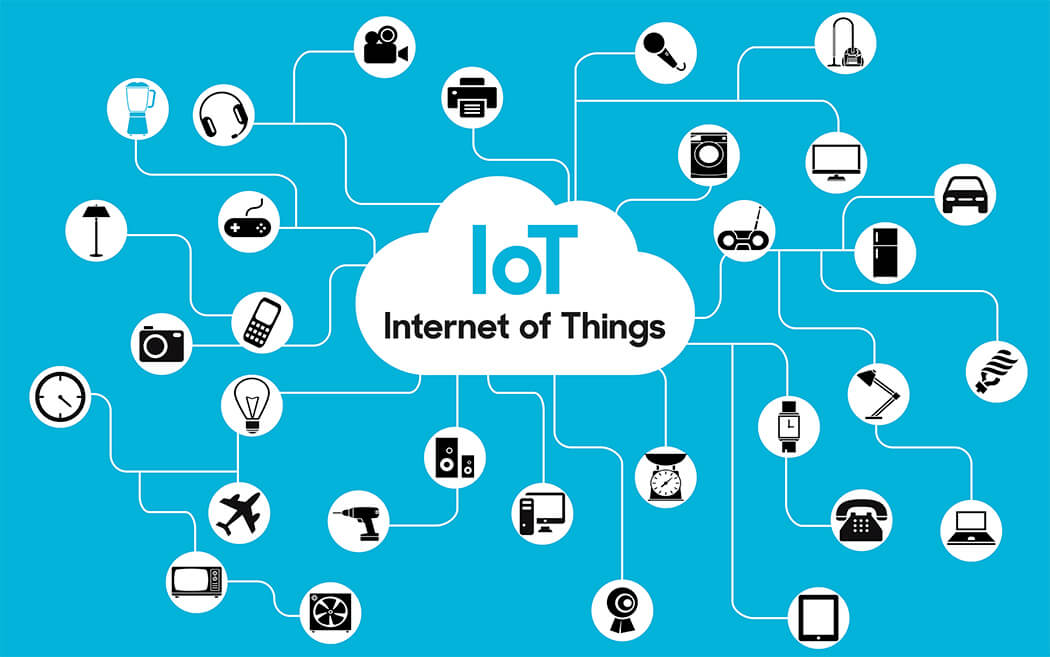
\includegraphics[width=0.9\textwidth]{figs/iot.jpg}}
        \caption{نمای کلی از اینترنت اشیاء}
        \label{fig:iot}
    \end{figure}
}

\section{معماری بازخوانی}
\label{sec:callback}
\paragraph{}
{
    نرم‌افزارهای مبتنی بر بازخوانی\footnote{\lr{Callback-Based Software}}، الگوها و روش‌هایی در برنامه‌نویسی هستند که در آن بخشی از کد به عنوان ورودی به یک تابع دیگر داده می‌شود، و آن تابع در زمان لازم، این ورودی را به صورت بازخوانی\footnote{\lr{Callback}} فراخوانی می‌کند. با این روش، کاربر می‌تواند اجرای برنامه را کنترل کند و در زمان‌های خاص، تابع مورد نظر خود را صدا کند.
    یکی از استفاده‌های متداول این الگو در پاسخ به وقوع رویدادها است. در این حالت، یک تابع بازخوانی به عنوان ورودی به یک رویداد مرتبط ارسال می‌شود. وقتی که رویداد رخ دهد، نرم‌افزار بازخوانی را فراخوانی می‌کند و عملیات مورد نظر را اجرا می‌کند. این روش به برنامه‌نویس امکان می‌دهد تا همزمان با اجرای دیگر بخش‌های برنامه، به رویدادها واکنش نشان دهد.
    در نرم‌افزارهای مبتنی بر بازخوانی، تعامل بین بخش‌های مختلف برنامه به صورت غیر همزمان انجام می‌شود. با این روش، برنامه‌نویس می‌تواند به طور کنترل شده تغییرات را پیگیری کند و اقدامات مناسبی را در زمان لازم انجام دهد. این الگو به برنامه‌نویسان امکان می‌دهد تا برنامه‌های پیچیده‌تر و قابل اطمینان‌تری را طراحی کنند، زیرا تعاملات غیر همزمان میان بخش‌ها را کنترل می‌کند و بهبود قابلیت اطمینان سیستم را فراهم می‌کند.
    بنابراین، نرم‌افزارهای مبتنی بر بازخوانی، با استفاده از تابع بازخوانی به عنوان مکانیزم اصلی برای تعامل بین بخش‌های مختلف برنامه، سبب افزایش انعطاف‌پذیری، کنترل و قابلیت اطمینان در طراحی و پیاده‌سازی نرم‌افزارها می‌شوند.
}
% !TeX root=main.tex

\chapter{کارهای مرتبط} \label{ch:related}
\thispagestyle{empty}


\section{مقدمه}
\label{sec:intro}
\paragraph{}
{
    در این فصل به معرفی کارهای مشابه و شرح
    رویکردهای مورد استفاده برای حل مساله‌ی پرسش‌و‌پاسخ تصویری می‌پردازیم.
    در ابتدا به بررسی روش‌های متفاوتی که برای حل مسئله پرسش‌وپاسخ تصویری 
    ارائه شد و سپس به کارهای مشابه با تولید پاسخ در پرسش‌وپاسخ تصویری
    و مجموعه داده‌های موجود در این زمینه پرداخته ‌شده است. در نهایت به 
    مدل‌های از پیش‌ آموزش داده شده در این زمینه می‌پردازیم.  
}

\section{
    روش‌های متفاوت حل مسئله پرسش‌وپاسخ تصویری
}
\label{sec:approches_vqa}
\paragraph{}{
    تا قبل از سال 2019 روش‌ها و رویکرد‌های متفاوتی ارائه شده که 
    بتوان ویژگی‌های تصویری و زبانی را در کنار یکدیگر قرار دهیم. به طور کلی
    این روش‌ها را می‌توان در 5 دسته طبقه بندی کرد. 
}
\subsection{
    روش‌های بر پایه 
    \lr{Bilinear Pooling}    
}
\label{sec:binilear_pooling}
\paragraph{}{
    روشی برای ایجاد توجه بین بردار‌های زبانی و بردار‌های تصویری است. 
    روش‌های 
    \r{Bilinear}
    بازنمایی خوبی را فراهم می‌کردند و در بسیاری از کارهای تصویری استفاده می‌شد. 
    در سال 2016
    روشی با نام 
    \lr{MCB}
    \cite{fukui-etal-2016-multimodal}
    برای ادغام تصویر و زبان ارائه شد. رویکرد آن‌ها در شکل 
    \ref{fig:mcb}
    نشان داده شده‌است. 
    \begin{figure}[H]
        \center{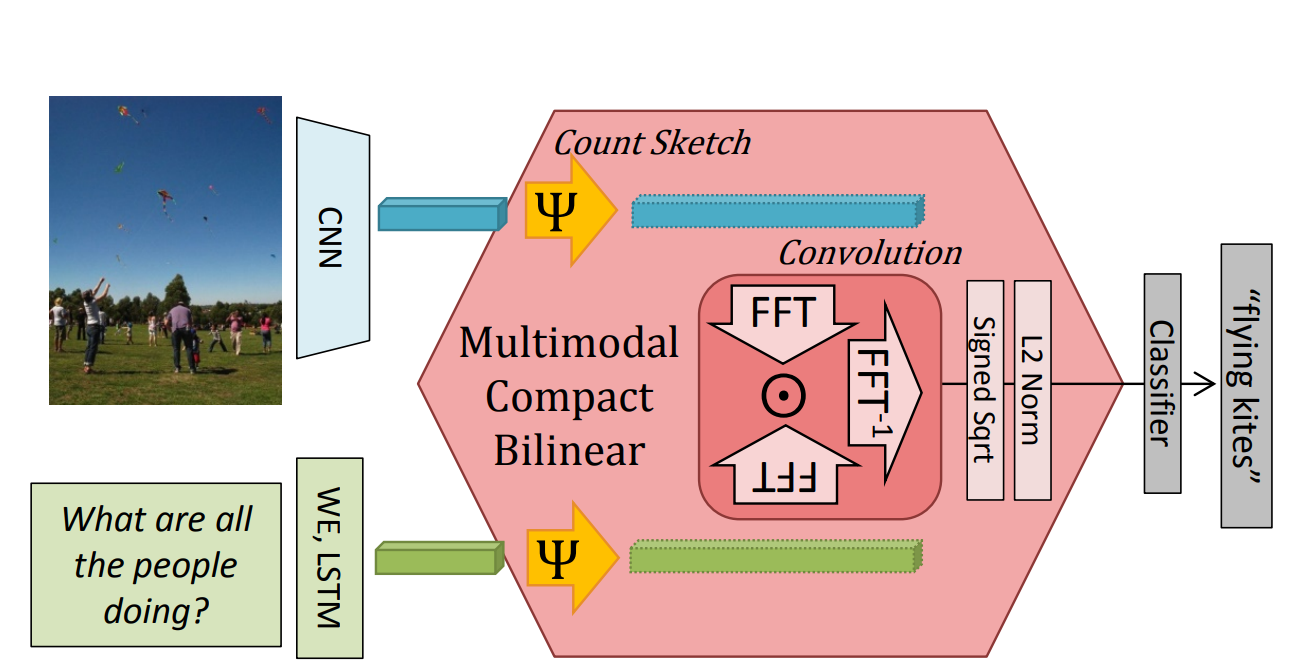
\includegraphics[width=0.7\textwidth]{figs/BiPooling.png}}
        \caption{روش \lr{MCB} برای ادغام تصویر و زبان}
        \label{fig:mcb}
    \end{figure}
    در سال 2017 نیز روشی از 
    دیگر
    با نام 
    \lr{MLB}
    \cite{kim2016hadamard}
    برپایه 
    \lr{Bilinear Pooling}
    را برای مسائل زبان و تصویر منتشر کرد که در زمان خود از 
    مدل‌های پایه‌ای عملکرد بهتری نشان داد. 
}

\subsection{
    روش‌های بر پایه توجه
}
\label{sec:attn_vqa_approach}
\paragraph{}{
    تا قبل از اینکه معماری‌های تبدیل‌کننده معرفی شوند،‌ محققان از مکانیزم توجه
    بر شبکه‌های عصبی بازگشتی و شبکه‌های کانولوشن استفاده می‌کردند، برای مثال
    شبکه‌ توجه پشته‌ای
    \cite{yang2016stacked}
    ،
    توجه سلسه‌مراتبی 
    \cite{NIPS2016_9dcb88e0}
    و 
    توجه متقارن
    \cite{nguyen2018improved}
    پس از ارائه مکانیزم‌های توجه منتشر شدند.
    همان‌طوری که از تصویر 
    \ref{fig:stacked_attention}
    مشخص است، توجه سلسله‌مراتبی 
    برای پردازش تصویر از یک شبکه‌ کانولوشن و برای پردازش سوال یا 
    همان بخش زبانی، از یک 
    \lr{LSTM}
    استفاده شده است، سپس با استفاده از مکانیزم پیشنهادی به تناظر میان این دو بخش
    پرداخته شده است. در هر دو پژوهش مجموعه داده‌های مشهور زبان و تصویر 
    ارزیابی شده‌ و نسبت به مدل‌های 
    \lr{SOTA}
    به خوبی عمل کرده بود. با این‌ حال، این مدل‌ها دارای اشتباهات بسیاری بودند و 
    نیازمند بهبود بودند تا اینکه مدل‌های تبدیل شونده منتشر شدند و 
    توانستند به دقت به نسبت بالاتری از این معماری‌ها برسند.
    \begin{figure}[H]
        \center{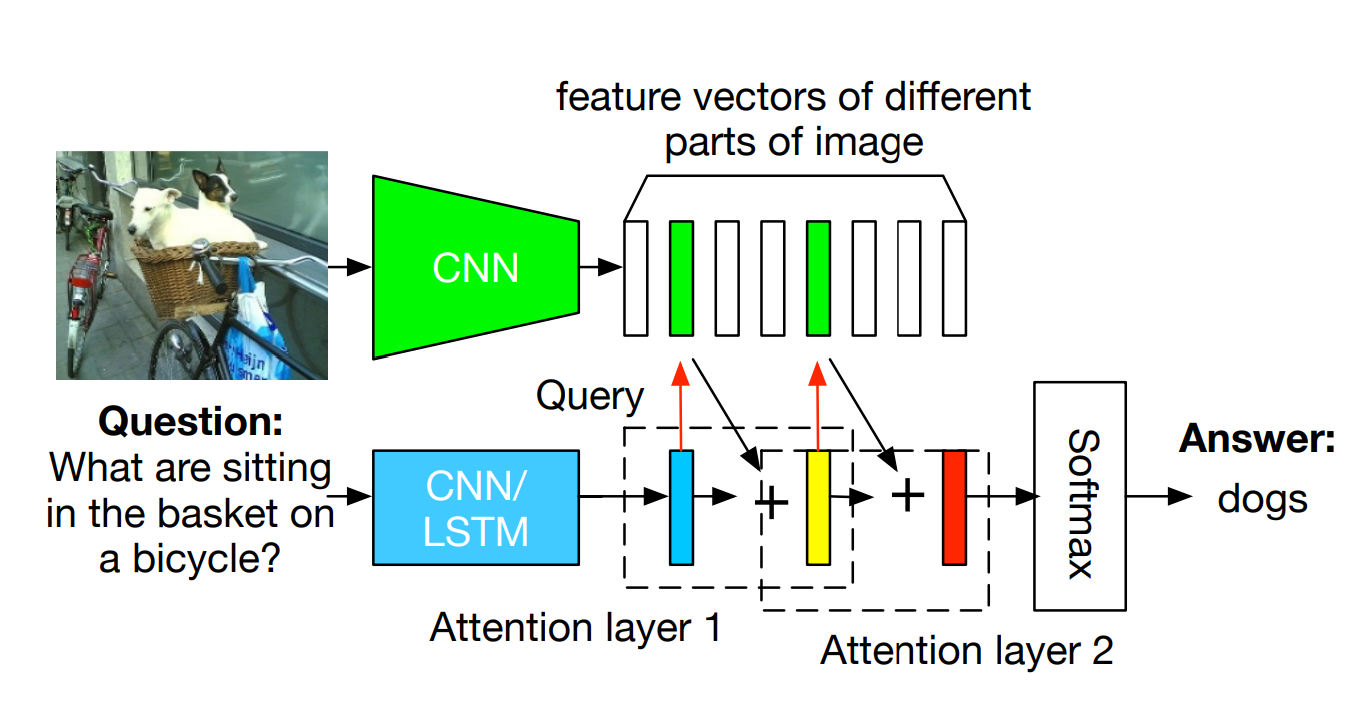
\includegraphics[width=0.7\textwidth]{figs/stacked_attention.png}}
        \caption{توجه پشته‌ای برای حل مسئله پرسش‌وپاسخ تصویری}
        \label{fig:stacked_attention}
    \end{figure}
}

\subsection{
    ادغام روابط اشیاء
}
\label{sec:object_relation_approach}
\paragraph{}{
    یکی از ایده‌های خلاقانه حل مسئله پرسش‌و‌پاسخ تصویری استفاده از شبکه‌های رابطه‌ای
    است که در ابتدا روابط بین اشیاء در تصویر و روابط بین کلمات در سوال مشخص
    می‌شوند و سپس به شبکه‌ای برای پیش‌بینی پاسخ مورد نظر ورودی داده می‌شوند. 
    از نمونه کارآمد این روش می‌توان به مفاله حل پرسش‌وپاسخ تصویری از طریق 
    ساختار گرافی 
    \cite{teney2017graph}
    اشاره کرد که در ابتدا اشیاء موجود در تصویر و روابط بین آن‌ها،‌
    و همچنین کلمات موجود در جمله سوال و روابط بین آن‌ها را
    به صورت گراف توصیف کرده و سپس آن‌ها به شبکه‌ عصبی ورودی می‌دهیم تا 
    بتواند از طریق آن‌ها به پاسخ مورد نظر برسد.
    برای بدست آوردن رابطه بین اشیاء در تصویر می‌توان از شبکه‌های رابطه‌ای 
    و برای بدست آوردن گراف جمله می‌توان از گراف وابستگی گرامری 
    استفاده کرد. 

    \begin{figure}[H]
        \center{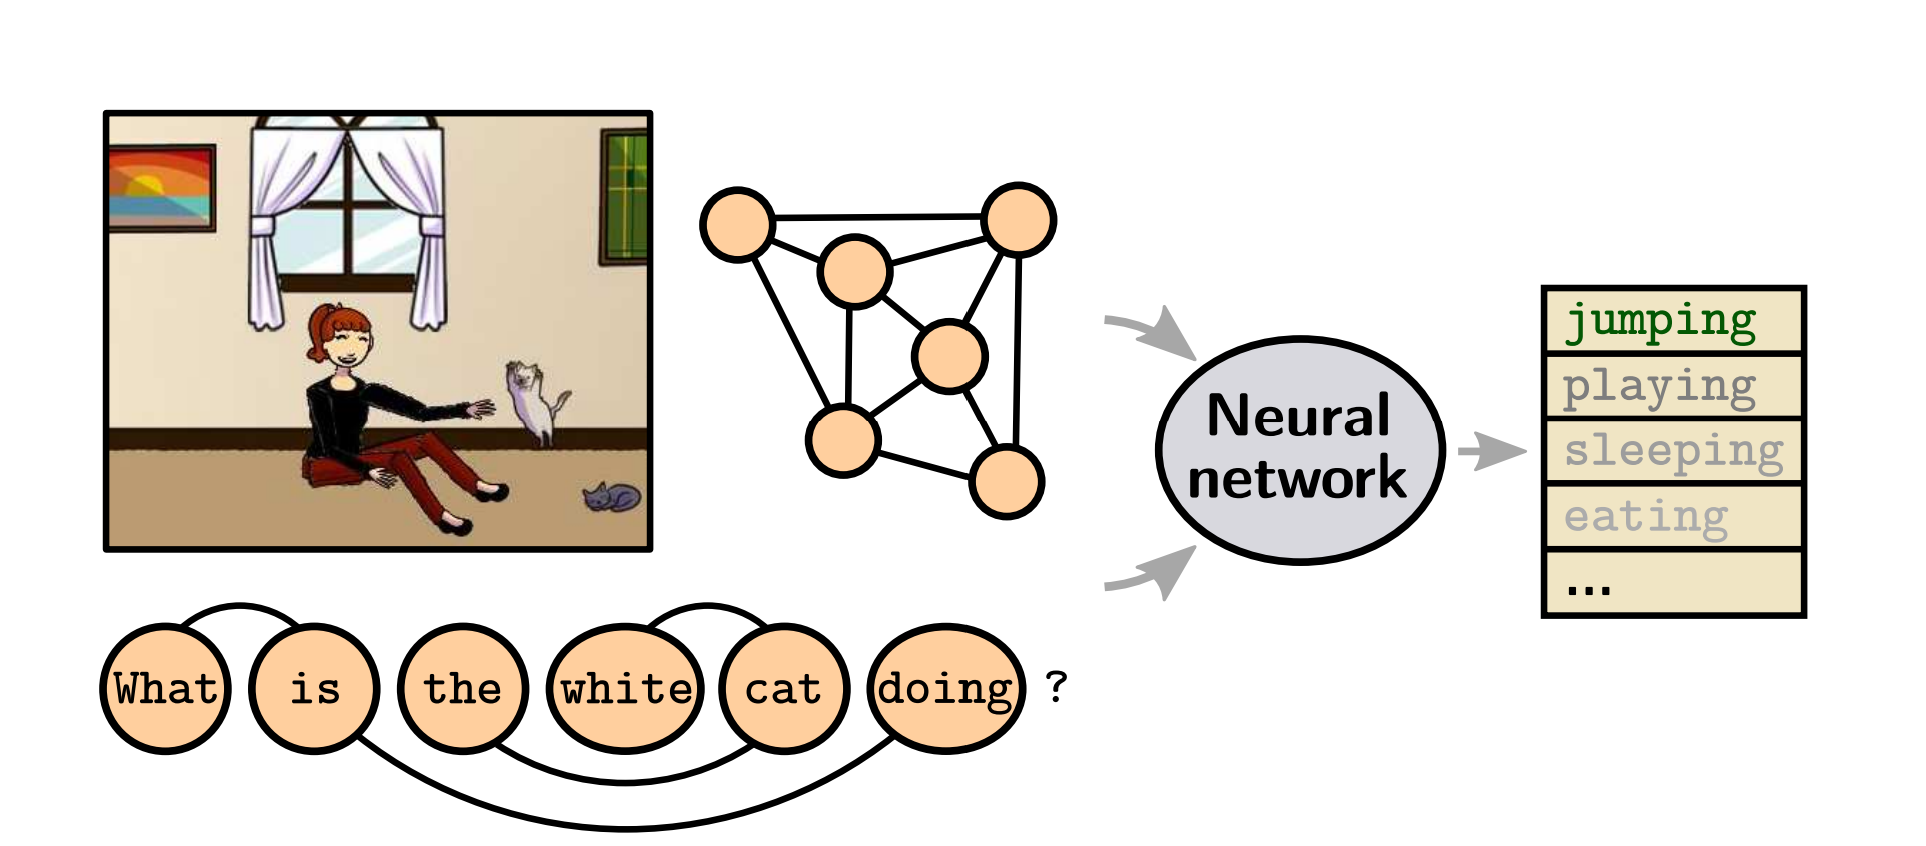
\includegraphics[width=0.7\textwidth]{figs/object_relation.png}}
        \caption{حل پرسش‌وپاسخ تصویری با ساختارهای گرافی}
        \label{fig:object_relation}
    \end{figure}
    
}

\section{
    تولید پاسخ برای پرسش‌و‌پاسخ تصویری
}
\label{sec:answer_generation}
\paragraph{}
{
    همان‌طوری که در بخش 
    \ref{sec:approches_vqa}
    توضیح داده‌شد، تلاش‌های بسیاری برای حل پرسش و پاسخ تصویری از طریق دسته‌بندی
    شده است، در حالی که حل مسئه از طریق تولید متن توجه چندانی از محققان را 
    جلب نکرده‌است. راه‌هایی برای حل پرسش‌وپاسخ تصویری با نام‌های
    \lr{mQA} \cite{gao2015you} 
    و
    \lr{AMA} \cite{wu2016ask} 
    ارائه شد که از شبکه‌های 
    \lr{LSTM} 
    برای تولید پاسخ استفاده شده بود. 
    پس از آن نیز سیستم‌هایی نظیر 
    \lr{SimVLM} \cite{wang2021simvlm}
    منتشر شد که هدف آن کاهش هزینه و پیچیدگی آموزش بود. در این 
    سیستم‌ها حل کردن مسائل مرتبط با زبان و تصویر به هر دو روش
    تولید پاسخ و دسته‌بندی بررسی شده است. 
    در نهایت، 
    \lr{VL-Bart} و \lr{VL-T5} \cite{pmlr-v139-cho21a}
    یک چهارچوب یکپارچه‌ای را ارائه کردند که توانایی آموزش 
    کار‌های متفاوتی در کنار یکدیگر را داشت. شکل
    \ref{fig:vl-bart}
    کارایی این چهارچوب را در بخش های مختلف نشان می دهد.
    این مدل‌ها نشان‌ دادند که
    حل کردن مسائل چند ماژول از طریق تولید متن عملکرد و کارایی بهینه‌تری 
    از دسته‌بندی دارد. با این حال، از آنجایی که 
    این مدل‌ها روی مجموعه داده پرسش‌وپاسخ تصویری 
    \cite{VQA}
    آموزش داده شده‌اند و پاسخ‌ها در این مجموعه داده به صورت دسته‌بندی داده
    شده است، همچنان پاسخ دادن به صورت جملات را در بر ندارند.
    \begin{figure}[H]
        \center{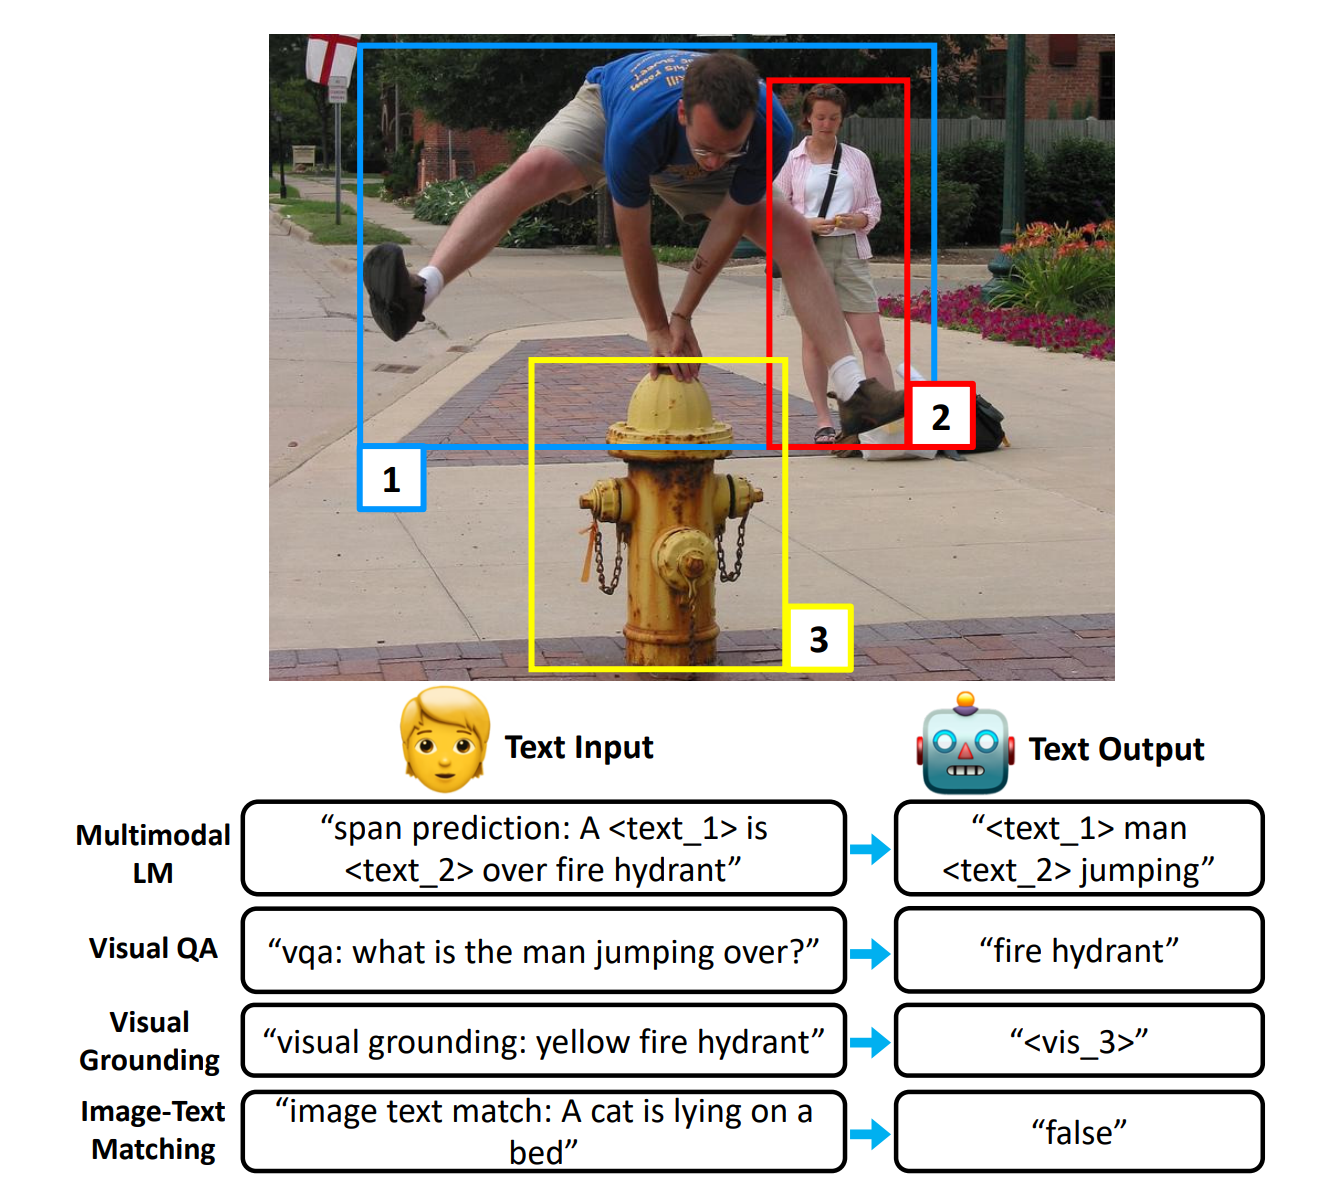
\includegraphics[width=0.7\textwidth]{figs/VL-BART.png}}
        \caption{چهارچوب یکپارچه ارائه شده برای حل مسائل چند ماژول به روش تولید متن}
        \label{fig:vl-bart}
    \end{figure}

}

\section{مجموعه داده‌های منتشر شده در پرسش‌وپاسخ تصویری}
\label{sec:vqa_datasets}
\paragraph{}
{
    مجموعه داده‌های زیادی در حوزه پرسش‌وپاسخ تصویری ارائه شده است. 
    با این حال، بسیاری از مجموعه داده‌ها دارای پاسخ‌های تک‌کلمه‌ای هستند 
    و تعداد کمی از آن‌ها پاسخ‌ها را به صورت جمله نوشته‌اند. 
    در سال 2019 مقاله 
    \lr{VCR} \cite{zellers2019recognition}
    ارائه شد که یک سوال چالشی از تصویری پرسیده شود و در جواب آن باید 
    پاسخی همراه با دلیل انتخاب پاسخ خروجی داده شود. 
    این مجموعه داده شامل 
    290 هزار 
    پرسش و پاسخ چند گزینه‌ای است که از 110 هزار صحنه فیلم‌ها گرفته شده است. 
    این مجموعه داده نشان داد که بر خلاف ساده بودن 
    \lr{VCR}
    برای انسان‌ها
    (دقتی بالاتر از 90)
    ماشین‌ها توانایی چندانی در حل آن ندارند. نویسندگان، مدلی نیز ارائه دادند که این
    مسئله را حل کند، ولی  طبق ادعای آن‌ها این مسئه همچنان فاصله زیادی تا حل دارد. 
    
    \begin{figure}[H]
        \center{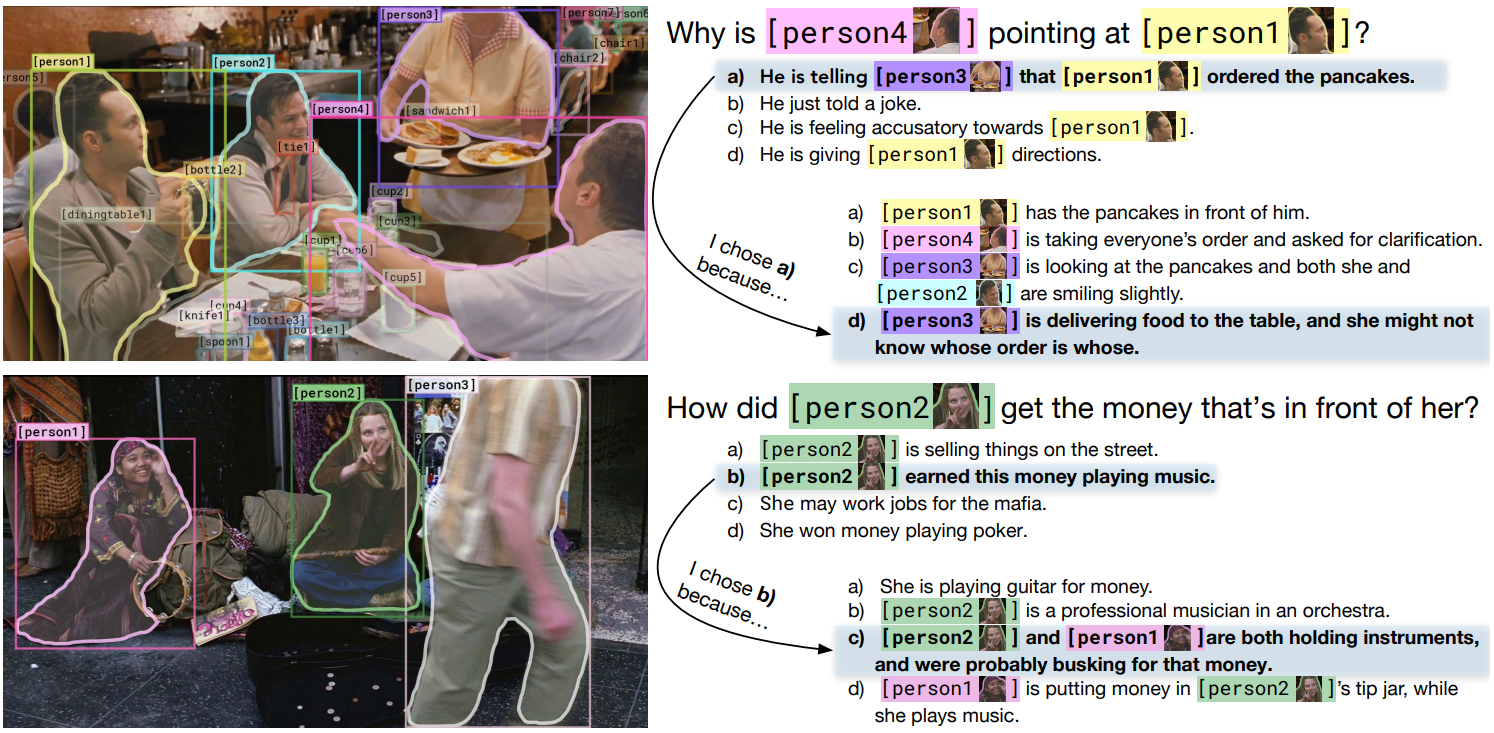
\includegraphics[width=1\textwidth]{figs/VCR.png}}
        \caption{نمونه‌ای مجموعه داده 
        \lr{VCR}
        که علاوه بر ارائه پاسخ، نیازمند ارائه دلیلی برای پاسخ است}
        \label{fig:vcr}
    \end{figure}
    مجموعه داده‌ دیگری با نام 
    \lr{VQA-E} \cite{li2018vqa}
    منتشر شد که برگرفته در مجموعه داده رسمی پرسش‌وپاسخ تصویری بود. 
    برای حل این مجموعه داده، علاوه بر ارائه پاسخ 
    (تک‌کلمه‌ای)
    باید توضیحی برای پاسخ انتخاب شده ارائه شود. نحوه تولید این مجموعه داده
    به این صورت است که به ازای هر سه‌تایی پرسش، تصویر و پاسخ یک توضیحی 
    با توجه به توضیحات تصویر تولید می‌شود. در این مجموعه داده، تلاش بر این بوده
    که توزیعی مشابه با مجموعه داده رسمی پرسش‌وپاسخ تصویری داشته باشد. 
    مجموعه داده‌های دیگری نیز به صورت جمعیت‌‌محور ارائه شده‌اند. این مدل مجموعه
    داده‌ها می‌توان به 
    \lr{A-OKVQA} \cite{schwenk2022okvqa}
    اشاره کرد که شامل 25 هزار پرسش است. 
}

\section{ مدل‌های از پیش آموزش‌ داده‌شده}
\label{sec:vlp}
\paragraph{}
{
    پیش‌آموزش مدل‌های زبان-تصویر اخیرا مورد توجه بسیاری واقع شده است. مدل‌های 
    موجود بیش‌تر بر پایه توجه به خود و معماری تبدیل شونده که در بخش ‌های
    \ref{subsec:self_attn}
    و
    \ref{sec:transformers}
    به صورت جزئی مورد بررسی قرار گرفته‌اند. این مدل‌ها در هر دو بخش 
    تصویر و زبان به خوبی عمل کرده‌اند. 
    همانطوری که در بخش
    \ref{sec:bertlike_arcs}
    توضیح داده‌شد، این مدل‌ها را می‌توان به دو بخش تک‌جریان و دو جریان دسته‌بندی 
    کرد. 
    با توجه به اینکه این مدل‌ها در تولید متن استفاده چندانی نداشته‌اند، در این
    پژوهش تلاش بر این بوده که مدل‌های از‌ پیش آموزش داده‌شده را برای این هدف 
    استفاده کنیم. 
}
% !TeX root=main.tex

\chapter{روش پیشنهادی} \label{ch:method}
\thispagestyle{empty}

\section{مقدمه}
\paragraph{}{
    % هدف اصلی پروژه امکان‌سنجی، طراحی، پیاده‌سازی و ارزیابی سامانه‌ای برای کنترل و پایش دستگاه‌های اینترنت اشیاء با استفاده از امکانات کوبلت مجازی بر سکوی کوبنیتز است.
    در این بخش، ابتدا معماری روش پیشنهاد را شرح داده و سپس اجزای مختلف آن را بررسی می‌کنیم. سپس به نحوه کارکرد این روش می‌پردازیم.
}

\section{معماری سامانه}
\paragraph{}{
    اجزای اصلی سامانه متشکل از پیاده‌سازی تامین‌کننده کوبلت مجازی، رابط بین تامین‌کننده و کنترل‌کننده‌ها، کنترل‌کننده‌ها و دستگاه‌ها می‌باشد که در ادامه به تعریف هرکدام پرداخته
    \begin{figure}[H]
        \center{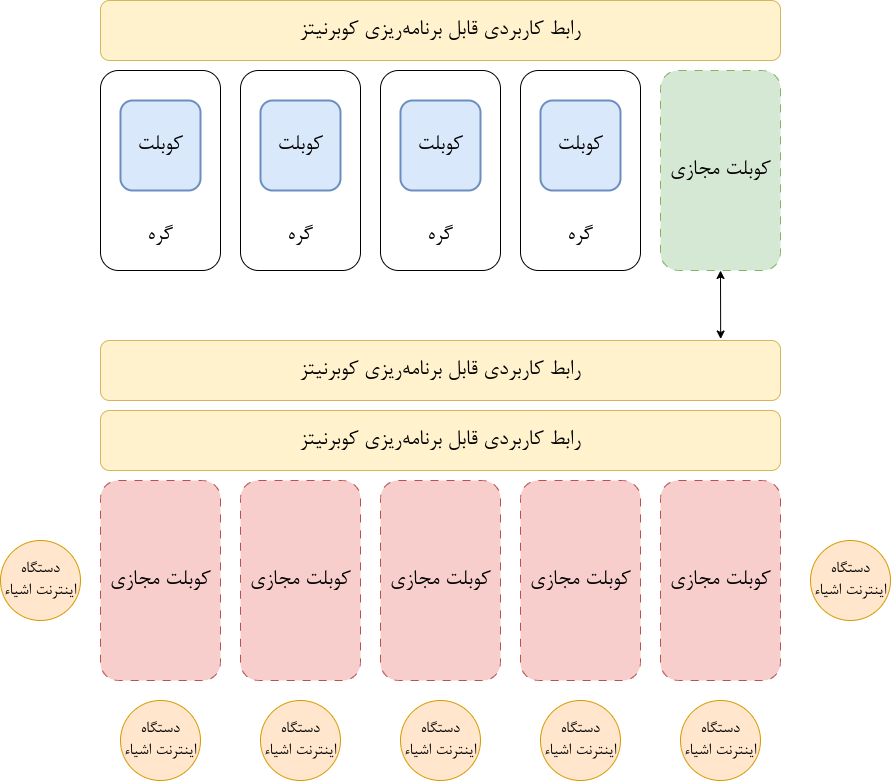
\includegraphics[width=0.8\textwidth]{figs/arch.png}}
        \caption{نمای کلی معماری}
        \label{fig:arch}
    \end{figure}
}
\subsection{پیاده‌سازی تامین‌کننده کوبلت مجازی}
\label{subsec:provider}
\paragraph{}
{
    کوبلت مجازی با در اختیار گذاشتن رابط‌هایی برای برنامه‌نویس، این امکان را می‌دهد که بتوان گره‌های کوبرنیتز با پشتوانه‌های
    سفارشی‌سازی شده داشته باشیم. برای مثال رابط زیر چرخه وجودی یک پاد را نشان می‌دهد. حال با پیاده‌سازی این رابط، ما این امکان
    را داریم که از ساخته‌شدن، بروزرسانی شدن، حذف شدن و حتی تغییر وضعیت‌های پاد‌های مورد نظر خود با خبر شویم.
    \newpage
    \begin{latin}
    \begin{lstlisting}[caption=پاد وجودی چرخه کنترل‌کننده رابط]
        type PodLifecycleHandler interface {
            CreatePod(ctx context.Context, pod *corev1.Pod) error
        
            UpdatePod(ctx context.Context, pod *corev1.Pod) error
        
            DeletePod(ctx context.Context, pod *corev1.Pod) error
        
            GetPod(ctx context.Context, namespace, name string) (*corev1.Pod, error)
        
            GetPodStatus(ctx context.Context, namespace, name string) (*corev1.PodStatus, error)
        
            GetPods(context.Context) ([]*corev1.Pod, error)
        }        
    \end{lstlisting}
    \end{latin}

    پیاده‌سازی این رابط امکان این را می‌دهد که بتوانیم یک پاد بر روی کوبرنیتز اعمال کرده و سپس بوسیله کوبرنیتز فراخوانی شده تا پاد مورد نظر را بسازیم. در  این پروژه یک پاد نقش یک دستگاه اینترنت اشیاء را دارد.
    همچنین برای ارسال وضعیت گره مجازی ساخته شده، نیاز به پیاده‌سازی رابط دیگری داریم.

    \begin{latin}
        \begin{lstlisting}[caption={گره وضعیت کنترل‌کننده رابط}]
            type NodeProvider interface {
                Ping(context.Context) error

                NotifyNodeStatus(ctx context.Context, cb func(*corev1.Node))
            }

        \end{lstlisting}
    \end{latin}

    پیاده‌سازی این رابط باعث می‌شود هنگامی که کد مربوطه در حال اجرا می‌باشد، گره مورد در نظر در خوشه کوبرنیتز بصورت آماده ظاهر شود و اگه این کد متوقف شود، بصورت غیر آماده ظاهر شود.
    بعد از ثبت این دو رابط و انجام چند مرحله دیگر، تامین‌کننده ما آماده استفاده می‌شود و بصورت یک گره در کوبرنیتز ظاهر خواهد شد.
    \begin{figure}[H]
        \center{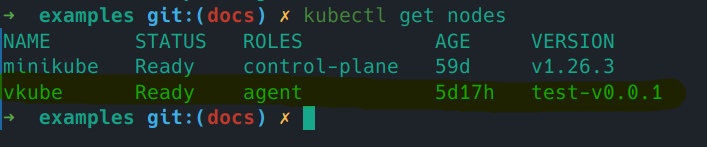
\includegraphics[width=0.8\textwidth]{figs/vkube_node.png}}
        \caption{گره مجازی}
        \label{fig:vkube_node}
    \end{figure}
}
\subsection{رابط برقراری ارتباط با کنترل‌کننده‌ها}
\label{subsec:connector}
\paragraph{}
{
    بعد از اتصال به کوبرنیتز و دریافت درخواست‌ها و بروزرسانی‌ها از سوی این سکو، باید با دستگاه‌های اینترنت اشیاء ارتباط برقرار کرده و وضعیتشان را در اختیار کوبرنیتز قرار دهیم.
    منطق ارتباط با کنترل‌کننده‌های دستگاه‌های اینترنت اشیاء به این صورت است که بصورت مداوم درخواست‌های خاصی به سمت کنترل‌کننده‌ها می‌فرستد تا از وضعیت خود کنترل‌کننده‌ها و همچنین دستگاه‌های اینترنت اشیاء تحت کنترلشان با خبر شود و درصورت نیاز کوبرنیتز را بروزرسانی کند. 
    این درخواست‌ها چیزی نیست جز درخواست‌های قرارداد انتقال فرا متن. همچنین برای اینکه بتوان تعداد زیادی دستگاه‌ اینترنت اشیاء را با یک کنترل‌کننده، کنترل کرد؛ از روش تکرار مقطعی استفاده شده است. این روش به ما کمک می‌کند تا وضعیت دستگاه‌ها را بصورت مقطعی (نه یکجا) دریافت کرده که بتوان در صورت امکان از همزمانی، برای تسریع کار، استفاده کرد.
    \\
    این رابط برای اینکه داده‌های مربوط به وضعیت دستگاه‌ها و کنترل‌کننده‌ها را در اختیار تامین‌کننده قرار دهد، از معماری بازخوانی\footnote{\lr{Callback}} استفاده می‌کند.
}

\subsection{شبیه‌ساز‍}
\label{subsec:simulator}
\paragraph{}
{
    در این پروژه یک شبیه‌ساز هم پیاده‌سازی شده که نقش کنترل‌کننده دستگاه‌های اینترنت اشیاء و همچنین خود این دستگاه‌ها را ایفا می‌کند. این شبیه‌ساز یک خدمت‌دهنده قرارداد انتقال فرامتن می‌باشد که امکانات زیر را هم برای کنترل‌کننده و هم برای دستگاه‌های اینترنت اشیاء فراهم می‌کند:
    \begin{enumerate}
        \item ساخت
        \item ساخت جمعی (برای ارزیابی ساده)
        \item بروزرسانی
        \item حذف
        \item دریافت تکی، همه و مقطعی
    \end{enumerate}
    دستگاه‌های اینترنت اشیاء شبیه‌سازی شده قفل‌های هوشمند یک ساختمان می‌باشند که امکان باز کردن و بستن قفل را دارند.
    \begin{figure}[H]
        \center{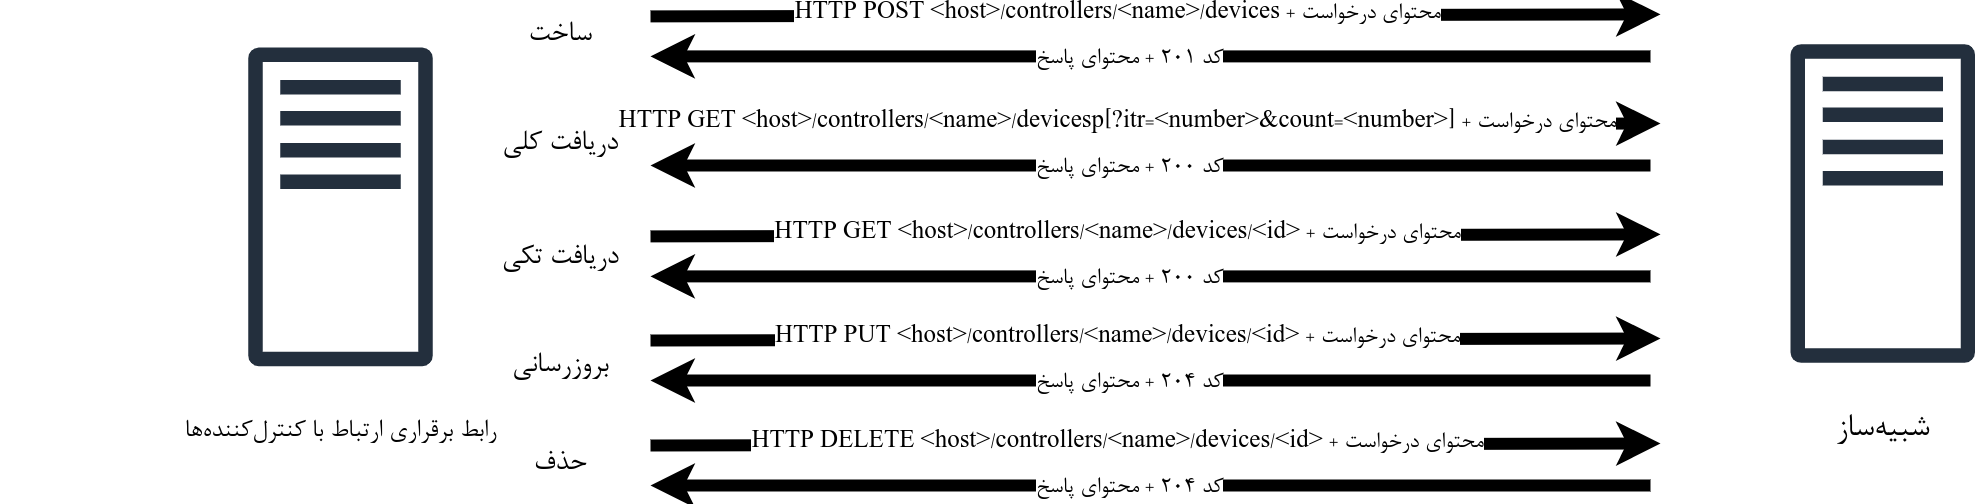
\includegraphics[width=\textwidth]{figs/sim_api.png}}
        \caption{رابط کاربردی قابل برنامه‌نویسی شبیه‌ساز}
        \label{fig:sim_api}
    \end{figure}
}

\subsection{رابط گرافیکی}
\label{subsec:gui}
\paragraph{}
{
    با توجه به اینکه هدف این پروژه امکان‌سنجی و پیاده‌سازی روشی برای پایش دستگاه‌های اینترنت اشیاء بوسیله بستر کوبرنیتز است، اما رابط گرافیکی نیز طراحی شد برای
    نمایش دادن هرچه بهتر اجزای پروژه. این رابط از دو بخش تشکیل شده است.
    \begin{enumerate}
        \item بخشی که با کنترل‌کننده دستگاه‌های اینترنت اشیاء ارتباط دارد و کمک به تسهیل ساخت و نمایش دستگاه‌‌های اینترنت اشیاء می‌کند.
        \item بخش دیگر که با تامین‌کننده در ارتباط است و بصورت مداوم وضعیت گره‌ها و پاد‌های مجازی را بروزرسانی می‌کند.
    \end{enumerate}

    \begin{figure}[H]
        \center{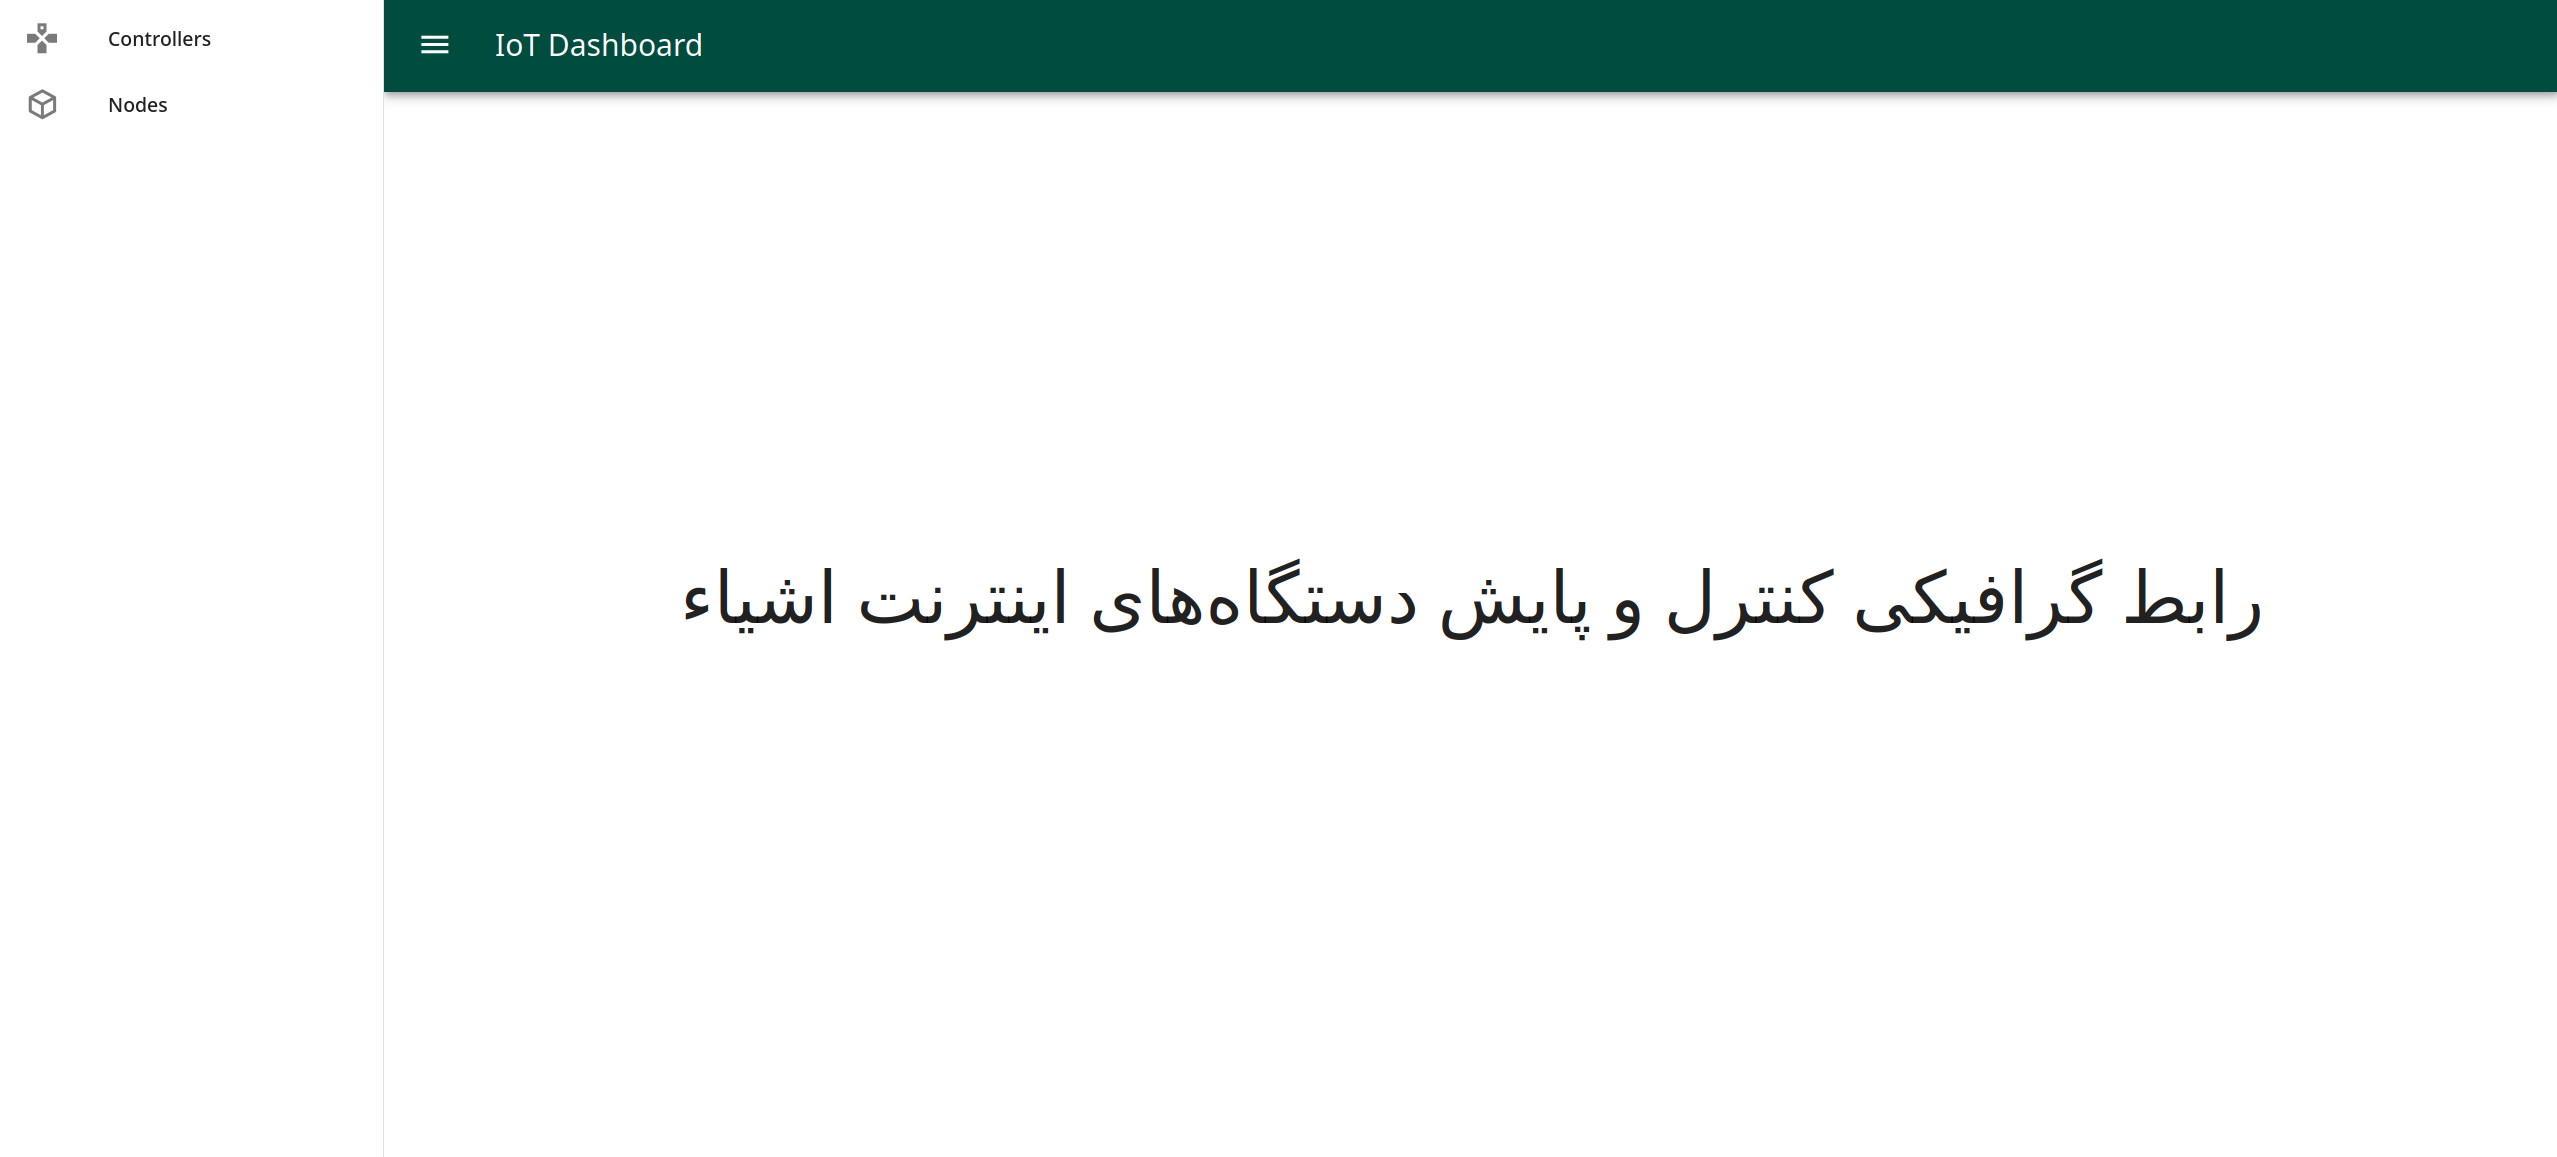
\includegraphics[width=\textwidth]{figs/dash_home.png}}
        \caption{صفحه اصلی رابط گرافیکی}
        \label{fig:dash_home}
    \end{figure}

    \begin{figure}[H]
        \center{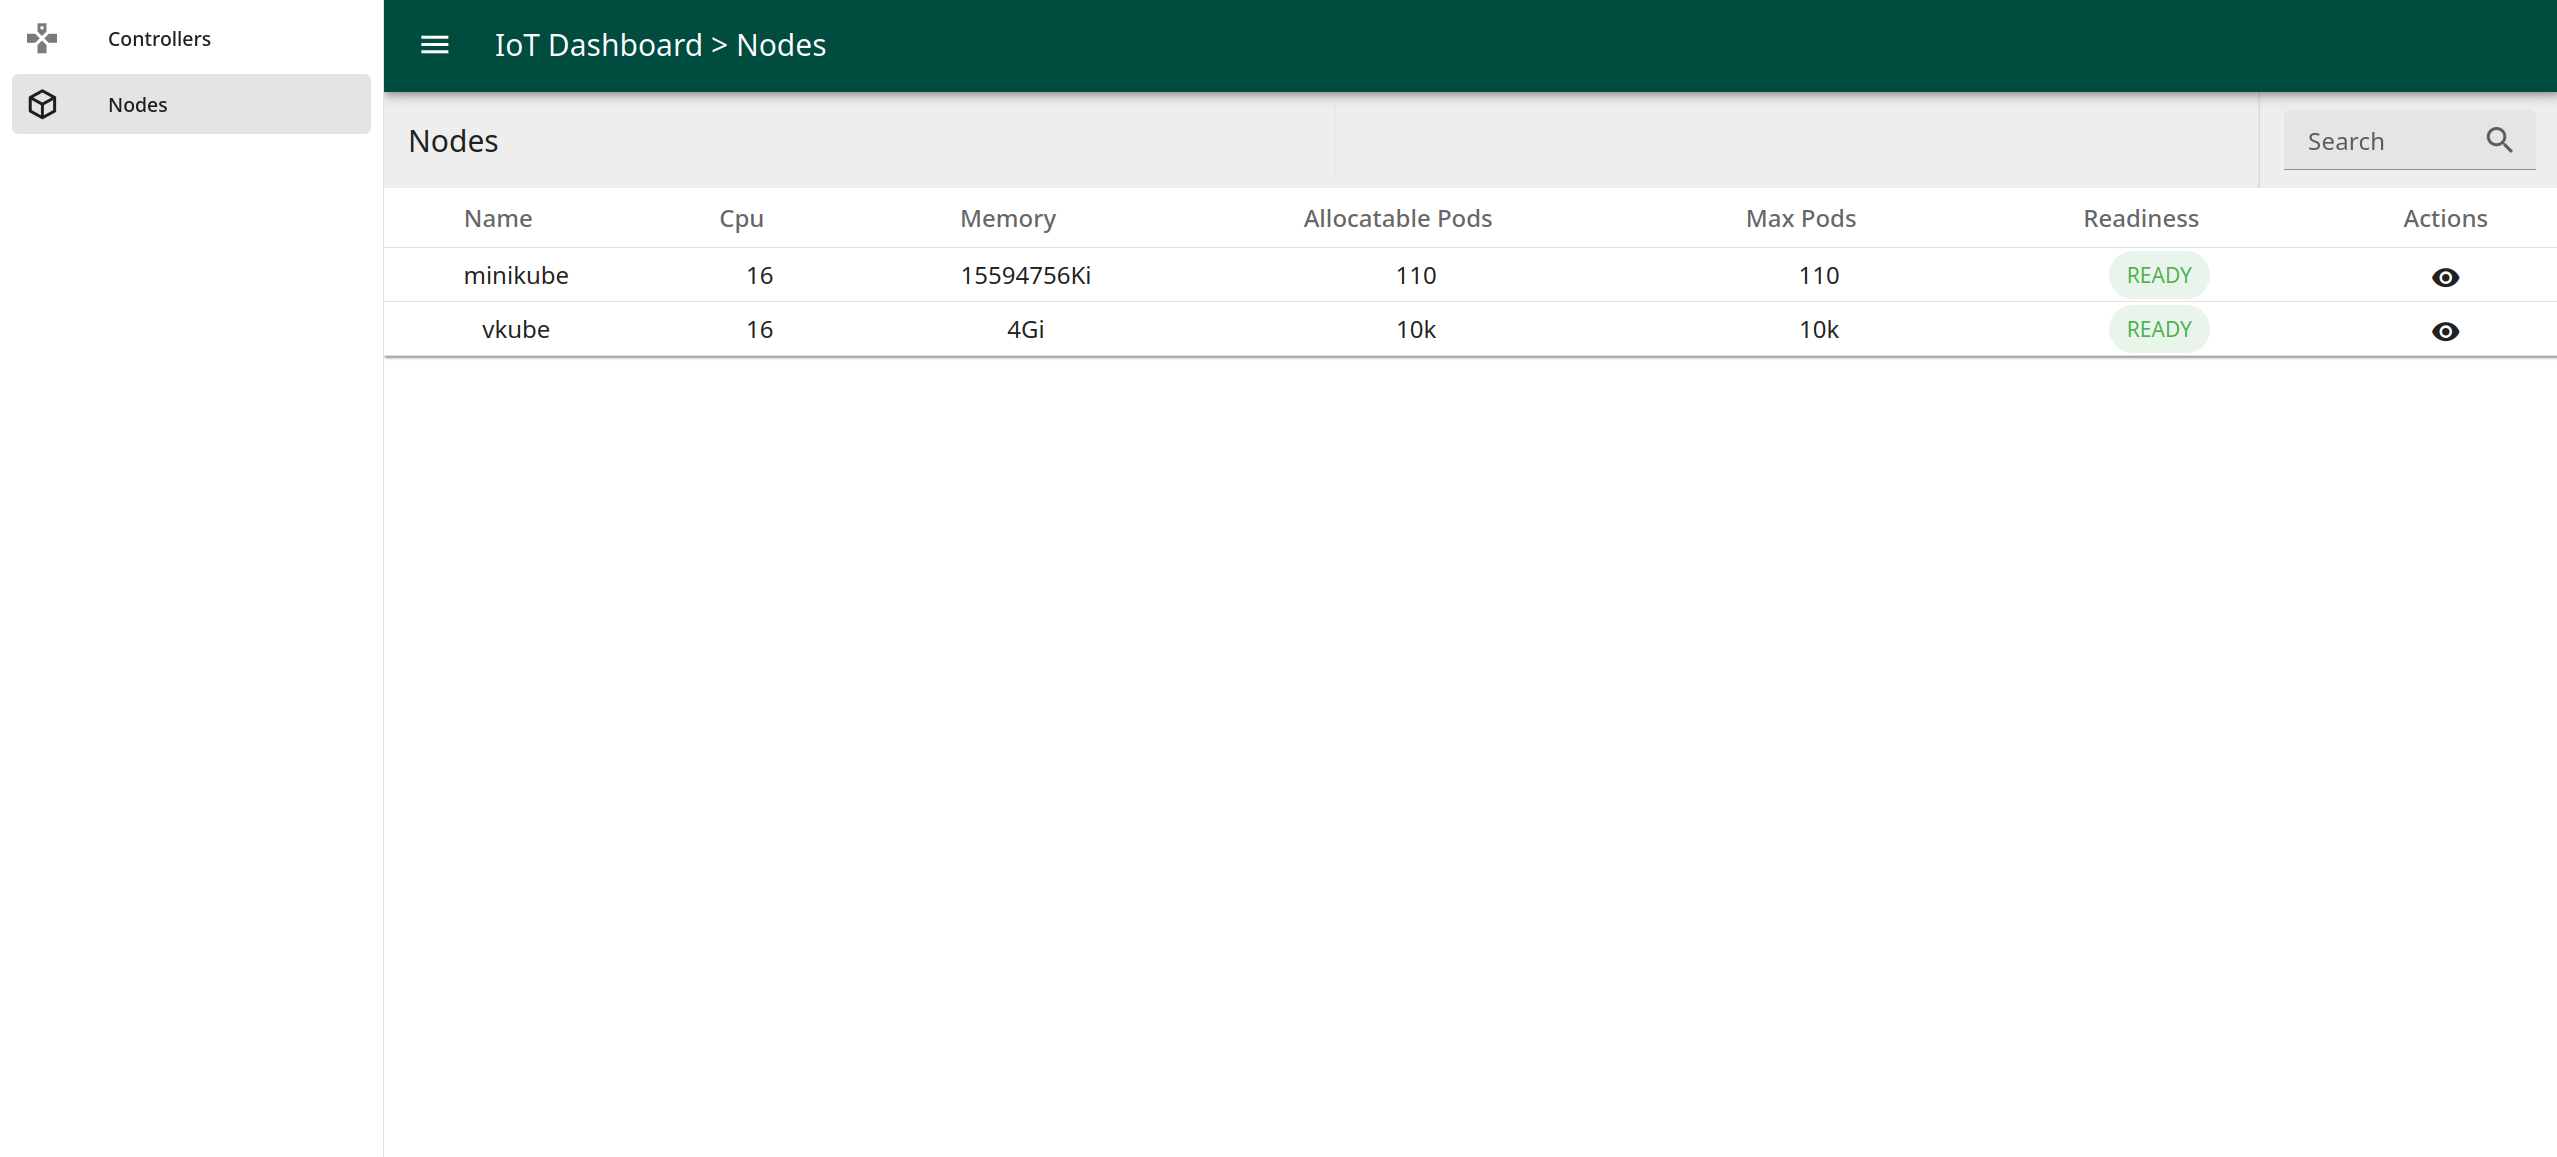
\includegraphics[width=\textwidth]{figs/dash_nodes.png}}
        \caption{صفحه گره‌های کوبرنیتز}
        \label{fig:dash_nodes}
    \end{figure}

    \begin{figure}[H]
        \center{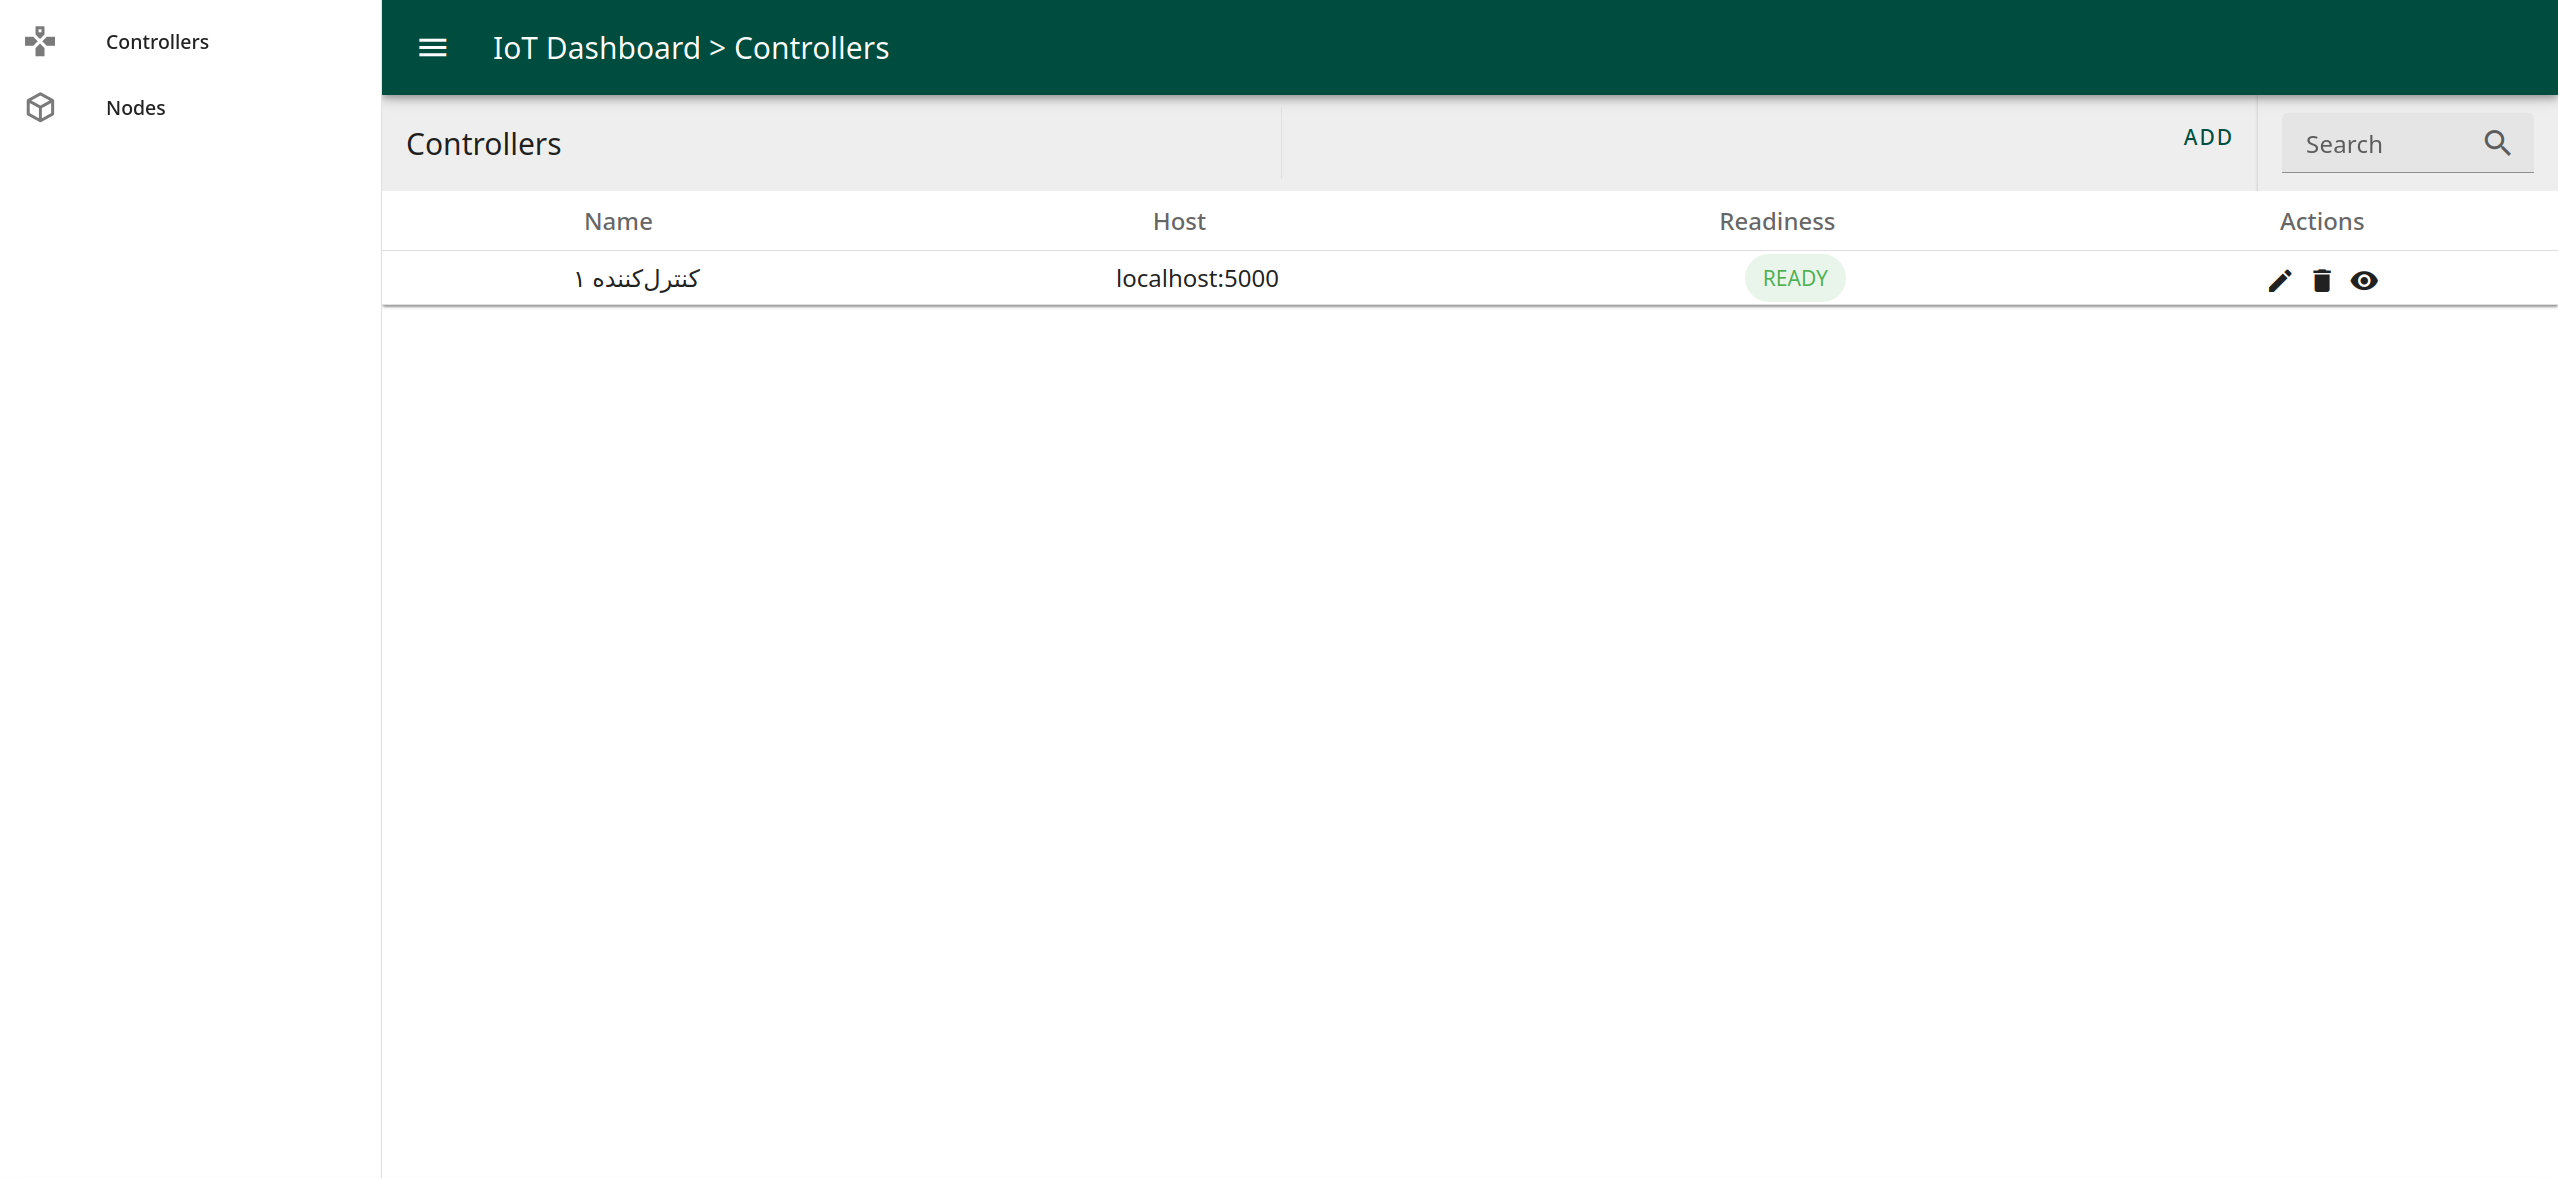
\includegraphics[width=\textwidth]{figs/dash_controllers.png}}
        \caption{صفحه کنترل‌کننده‌های کوبرنیتز کوبرنیتز}
        \label{fig:dash_controllers}
    \end{figure}
}


\section{نحوه کارکرد}
\paragraph{}
{
    ابتدا باید یک مستند پاد که در ذیل آمده مهیا کرده و در کوبرنیتز اعمال کنیم. بعد از اعمال این مستند،
    کوبرنیتز تامین‌کننده را از ایجاد این مستند با خبر می‌کند. حال تامین کننده با بازفراخوانی رابط کنترل‌کننده‌ها
    منجر به شروع دریافت وضعیت این دستگاه اینترنت اشیاء بصورت مداوم از کنترل‌کننده تعریف شده در مستند می‌شود.
    بنابراین رابط کنترل‌کننده‌ها بصورت مداوم با رابط کاربردی قابل برنامه‌نویسی شبیه‌ساز ارتباط گرفته و وضعیت دستگاه‌ها
    را بروزرسانی می‌کند.
    \newpage
    \begin{latin}
        \begin{lstlisting}[caption=کوبرنیتز در پاد ساخت مستند]
            apiVersion: v1
            kind: Pod
            metadata:
              name: lock-main
              annotations:
                controllerName: "controller1" 
                controllerAddress: "localhost:5000"
            spec:
              containers:
              # this is so that kubernetes validation will pass
                - image: doesntmatter/smart_lock
                  name: lock1
              dnsPolicy: ClusterFirst
              nodeSelector:
                kubernetes.io/role: agent
                kubernetes.io/os: linux
                type: virtual-kubelet
              tolerations:
              # this will target Virtual Kubelets nodes only
                - key: itzloop.dev/virtual-kubelet
                  operator: Exists
        \end{lstlisting}
    \end{latin}
    \newpage
    قبل از اعمال مستند بالا، از طریق رابط گرافیکی در  شبیه‌ساز چهار دستگاه ساخته که در شکل زیر مشاهده می‌کنید.
    \begin{figure}[H]
        \center{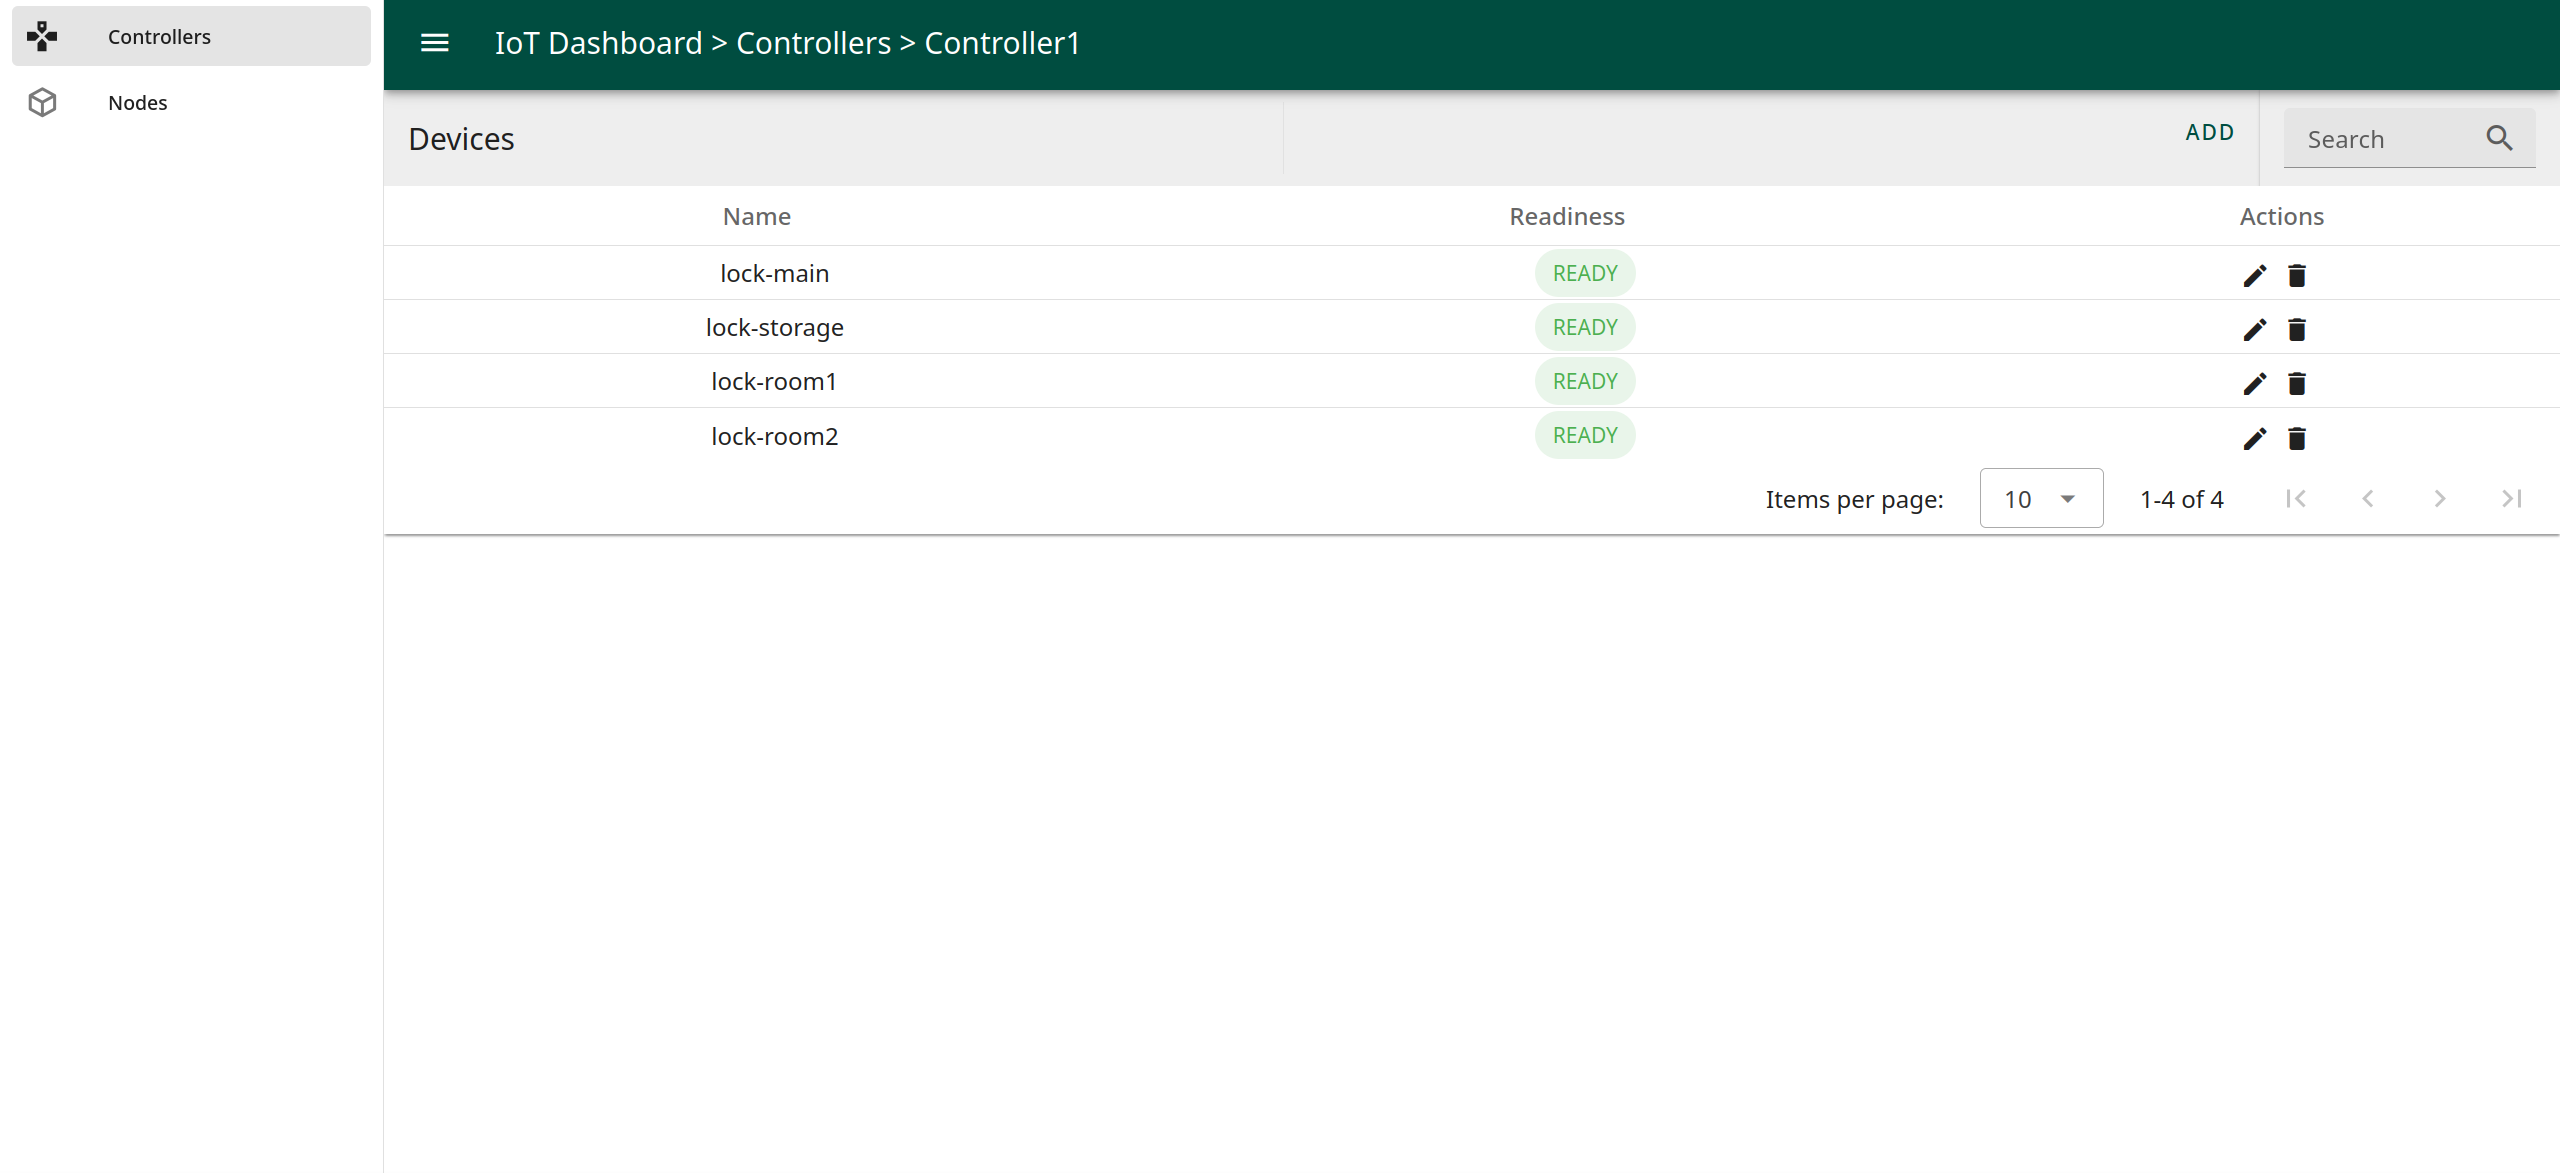
\includegraphics[width=\textwidth]{figs/dash_devices.png}}
        \caption{دستگاه‌های اینترنت اشیاء ساخته شده در شبیه‌ساز}
        \label{fig:dash_devices}
    \end{figure}
    در ادامه مستند پاد را اعمال می‌کنیم. همانطور که در مستند آماده است فقط یکی از این دستگاه‌ها یعنی قفل مرکزی\footnote{lock-main} را از طریق کوبرنیتز رصد می‌کنیم. بعد از اعمال این مستند پاد‌های کوبرنیتز را مشاهده‌ کرده که ابتده در وضعیت عدم آمادگی\footnote{\lr{Not-Ready}} می‌باشند.
    \begin{figure}[H]
        \center{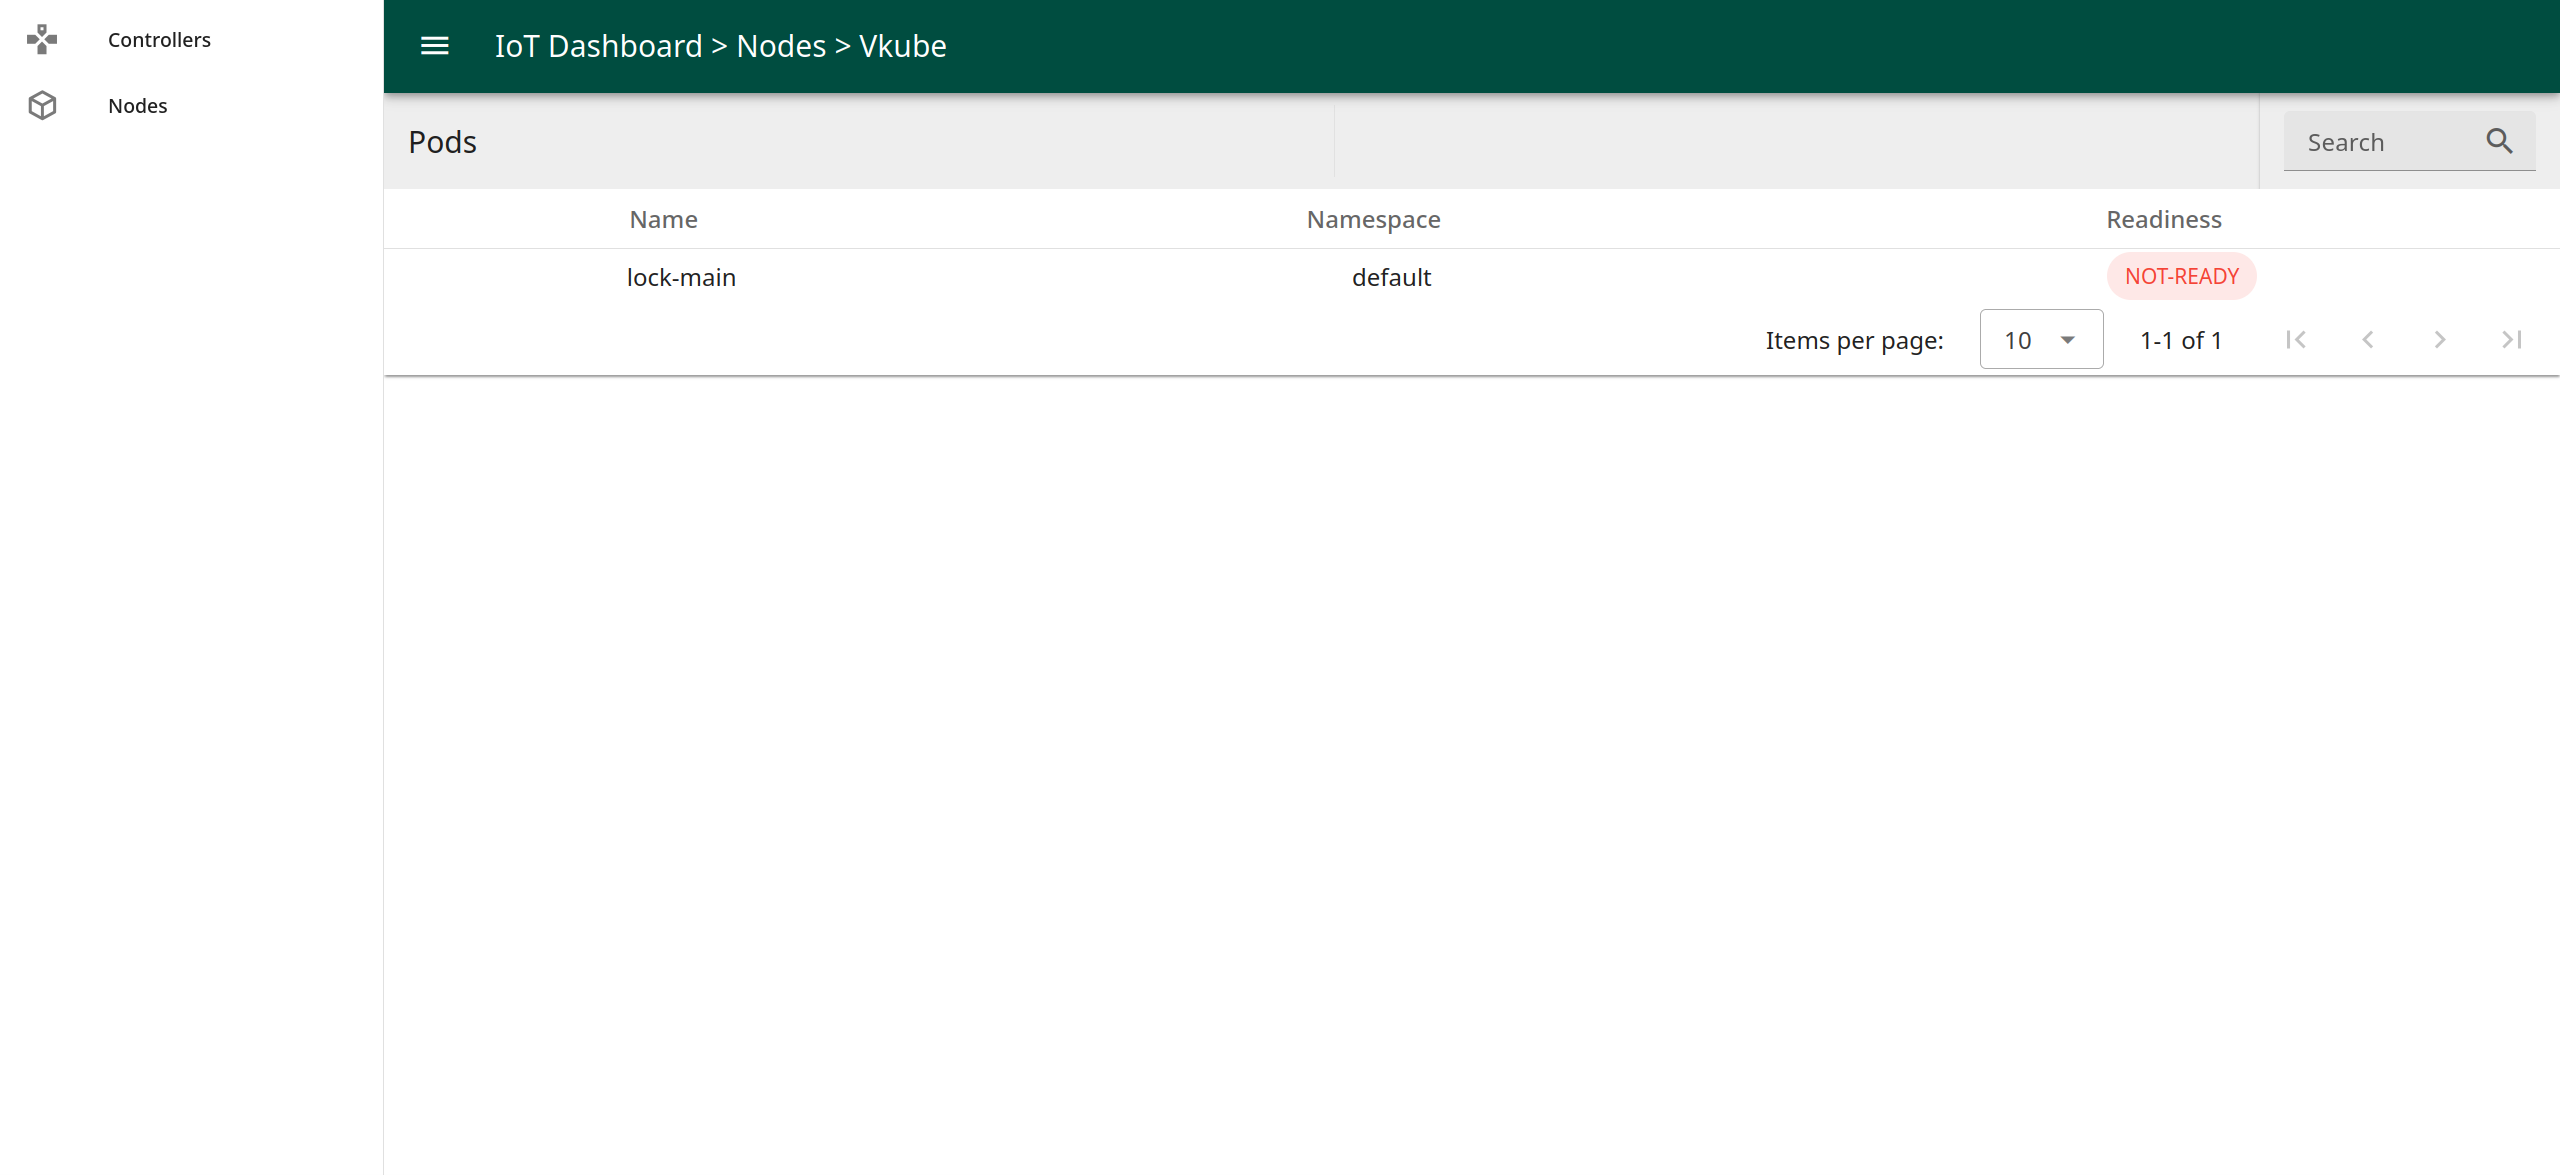
\includegraphics[width=\textwidth]{figs/dash_pod_lock_main_not_ready.png}}
        \caption{پاد ساخته شده از روی مستند در وضعیت عدم آمادگی}
        \label{fig:dash_pod_lock_main_not_ready}
    \end{figure}
    پس از گذر مدتی (مدت زمانی که طول می‌کشد رابط ارتباط با کنترل‌کننده‌ها وضعیت قفل مرکزی را از شبیه‌ساز دریافت کند) خواهیم دید که پاد مورد نظر در کوبرنیتز به وضعیت آماده\footnote{\lr{Ready}} در می‌آید.
    \begin{figure}[H]
        \center{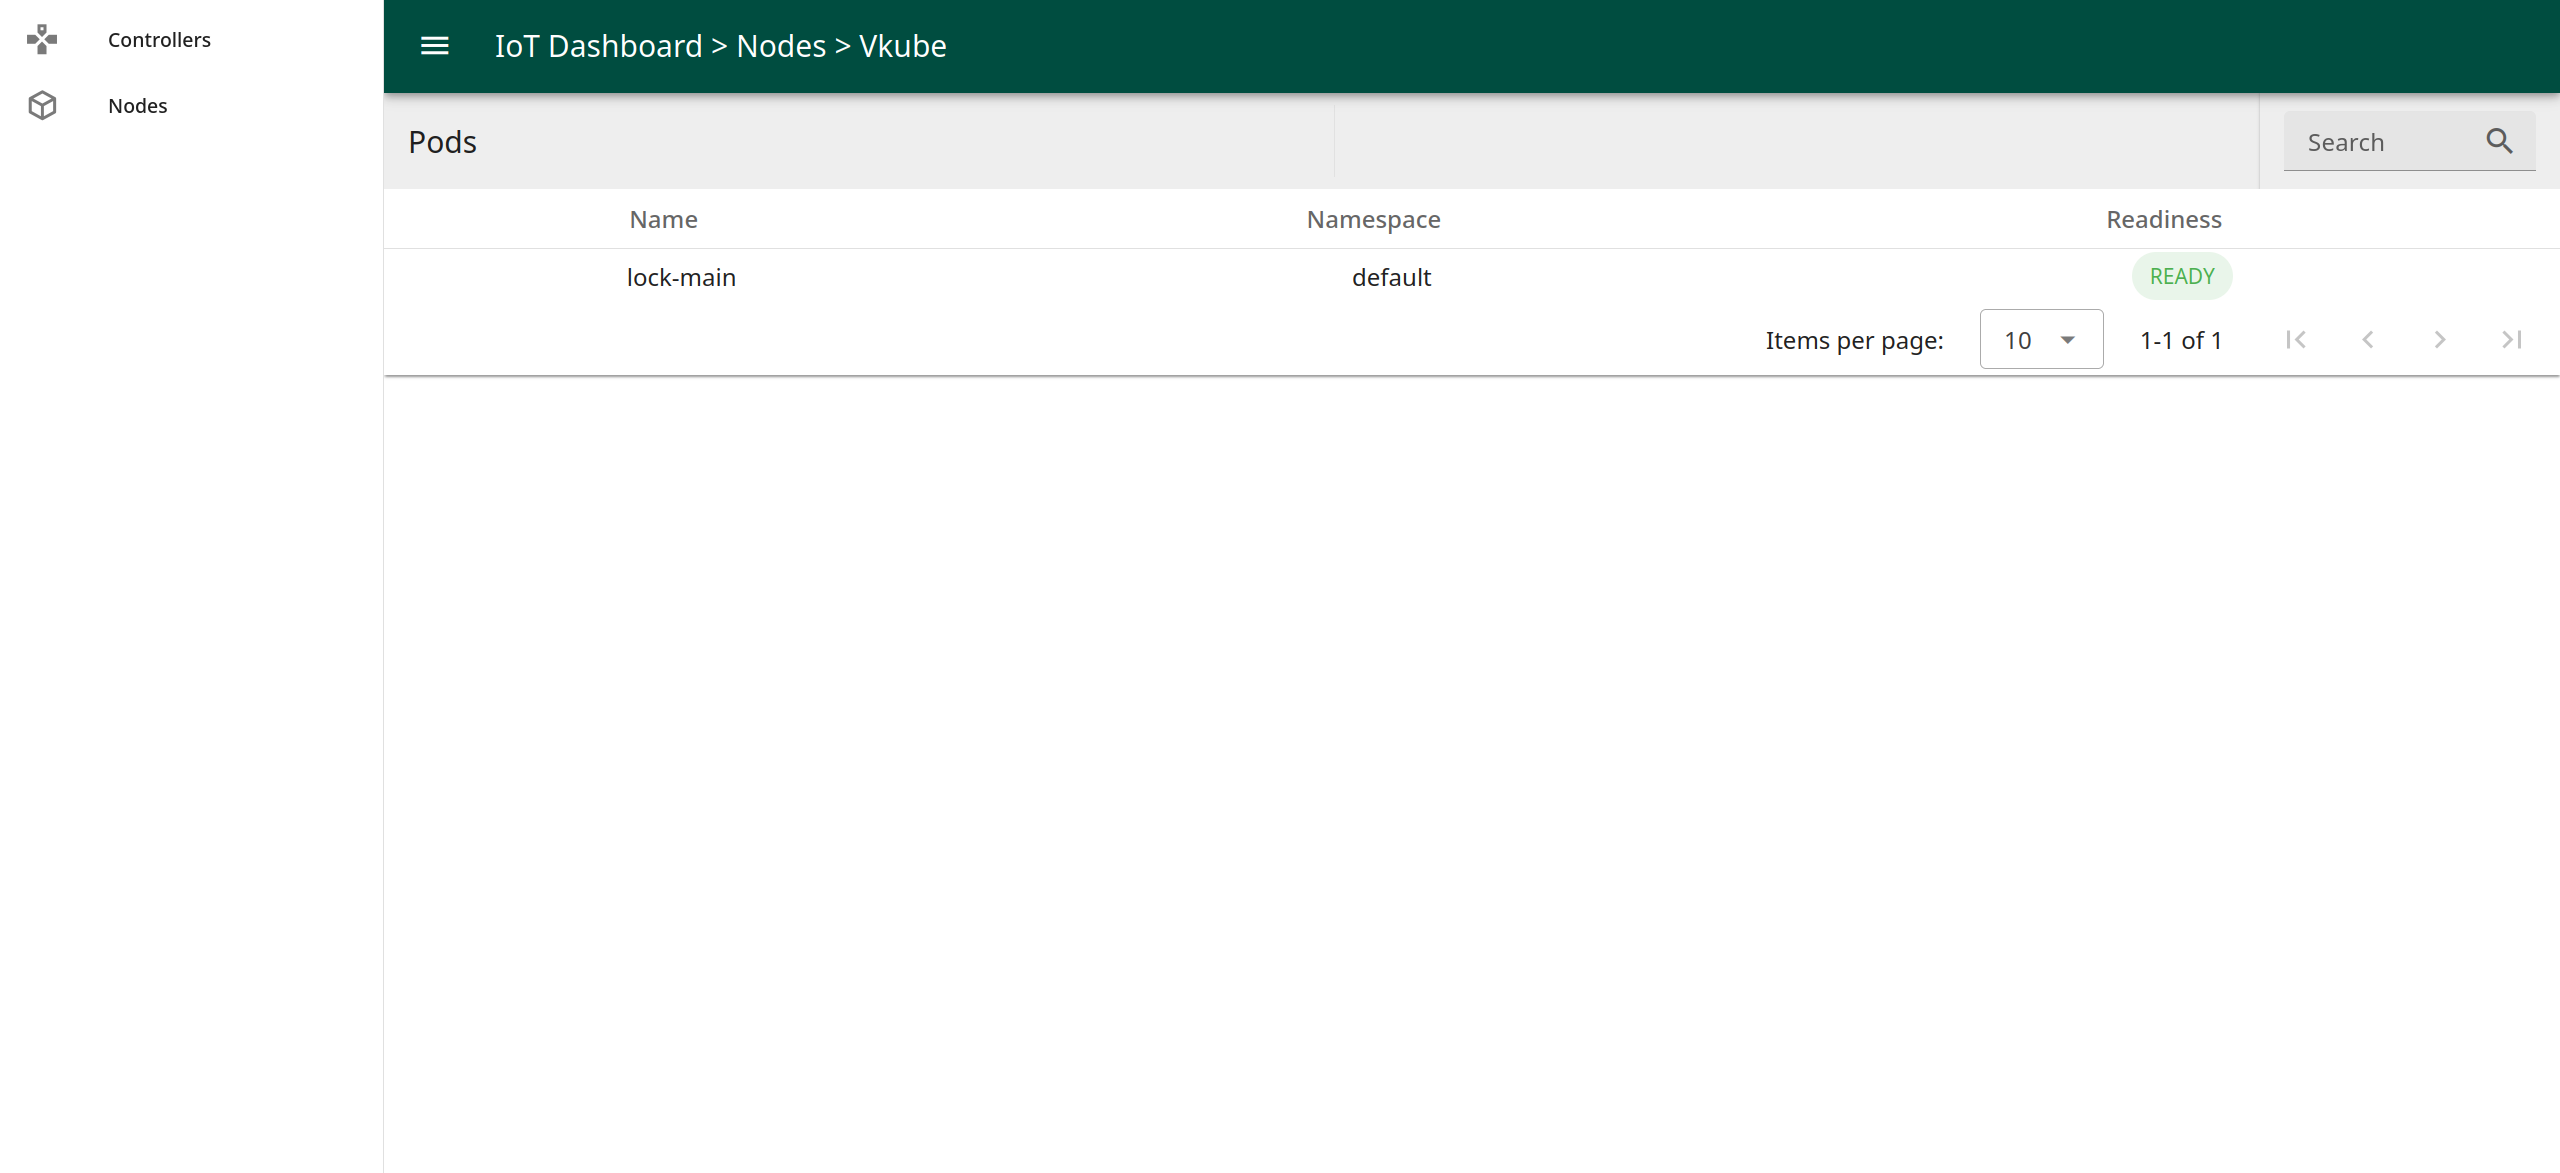
\includegraphics[width=\textwidth]{figs/dash_pod_lock_main_ready.png}}
        \caption{پاد ساخته شده از روی مستند در وضعیت آماده}
        \label{fig:dash_pod_lock_main_ready}
    \end{figure}

    حال اگر با استفاده از رابط گرافیکی، وضعیت قفل مرکزی در شبیه‌ساز را به وضعیت عدم آمادگی تغییر دهیم خواهیم دید که بعد از مدتی وضعیت پاد نیز تغییر می‌کند.
    \begin{figure}[H]
        \center{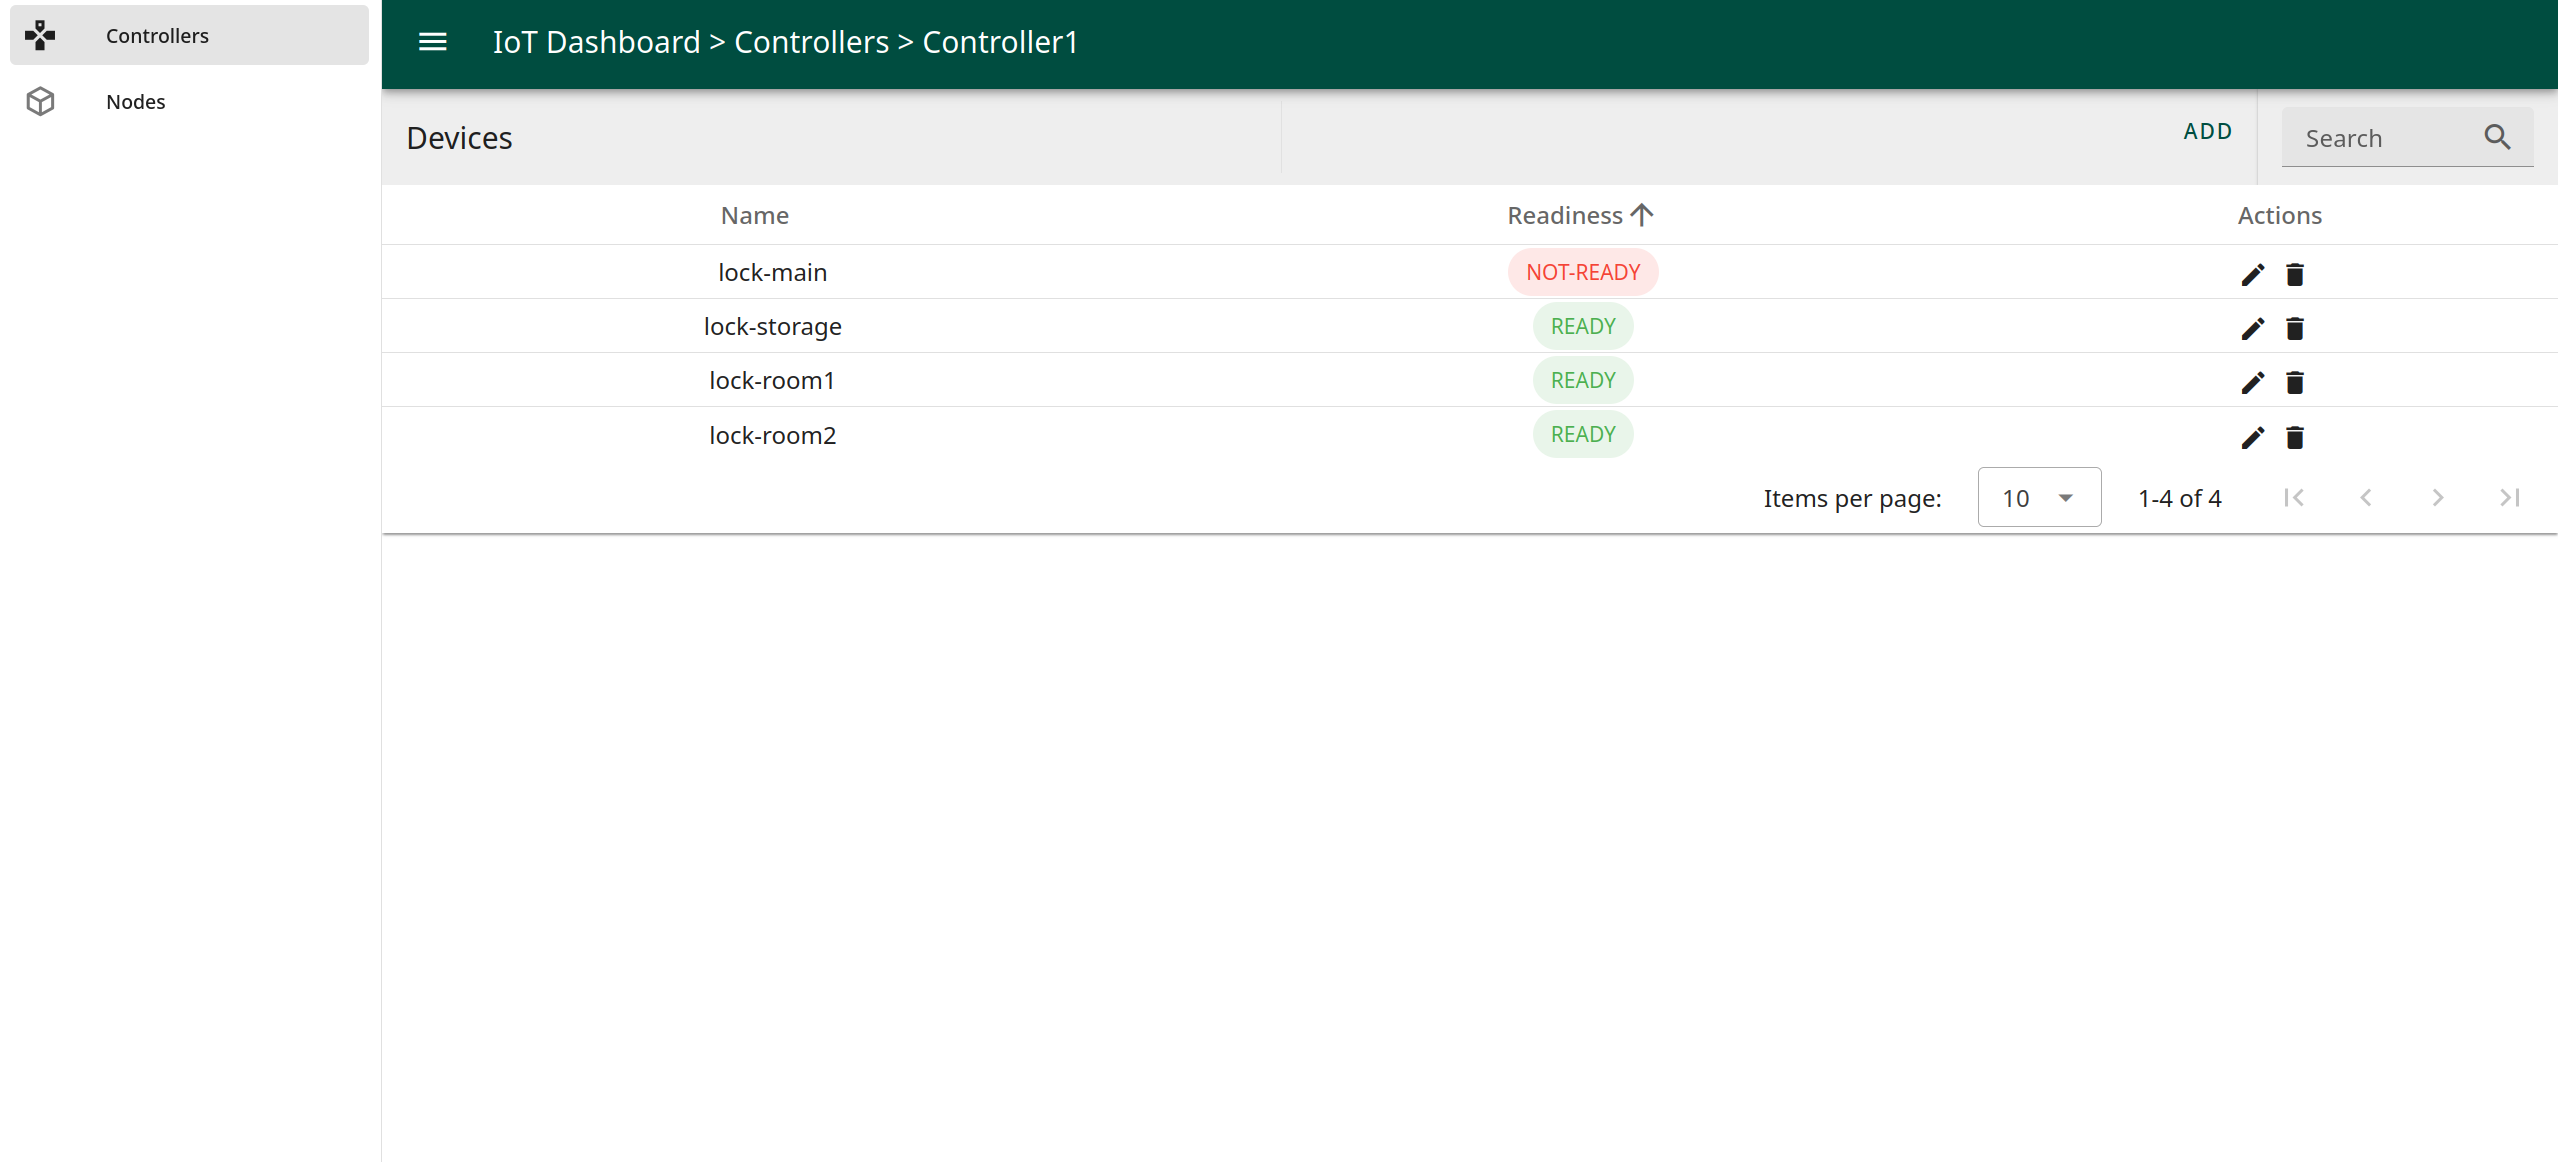
\includegraphics[width=\textwidth]{figs/dash_lock_main_change_readiness.png}}
        \caption{تغییر وضعیت قفل مرکزی در رابط گرافیکی}
        \label{fig:dash_lock_main_change_readiness}
    \end{figure}

    \begin{figure}[H]
        \center{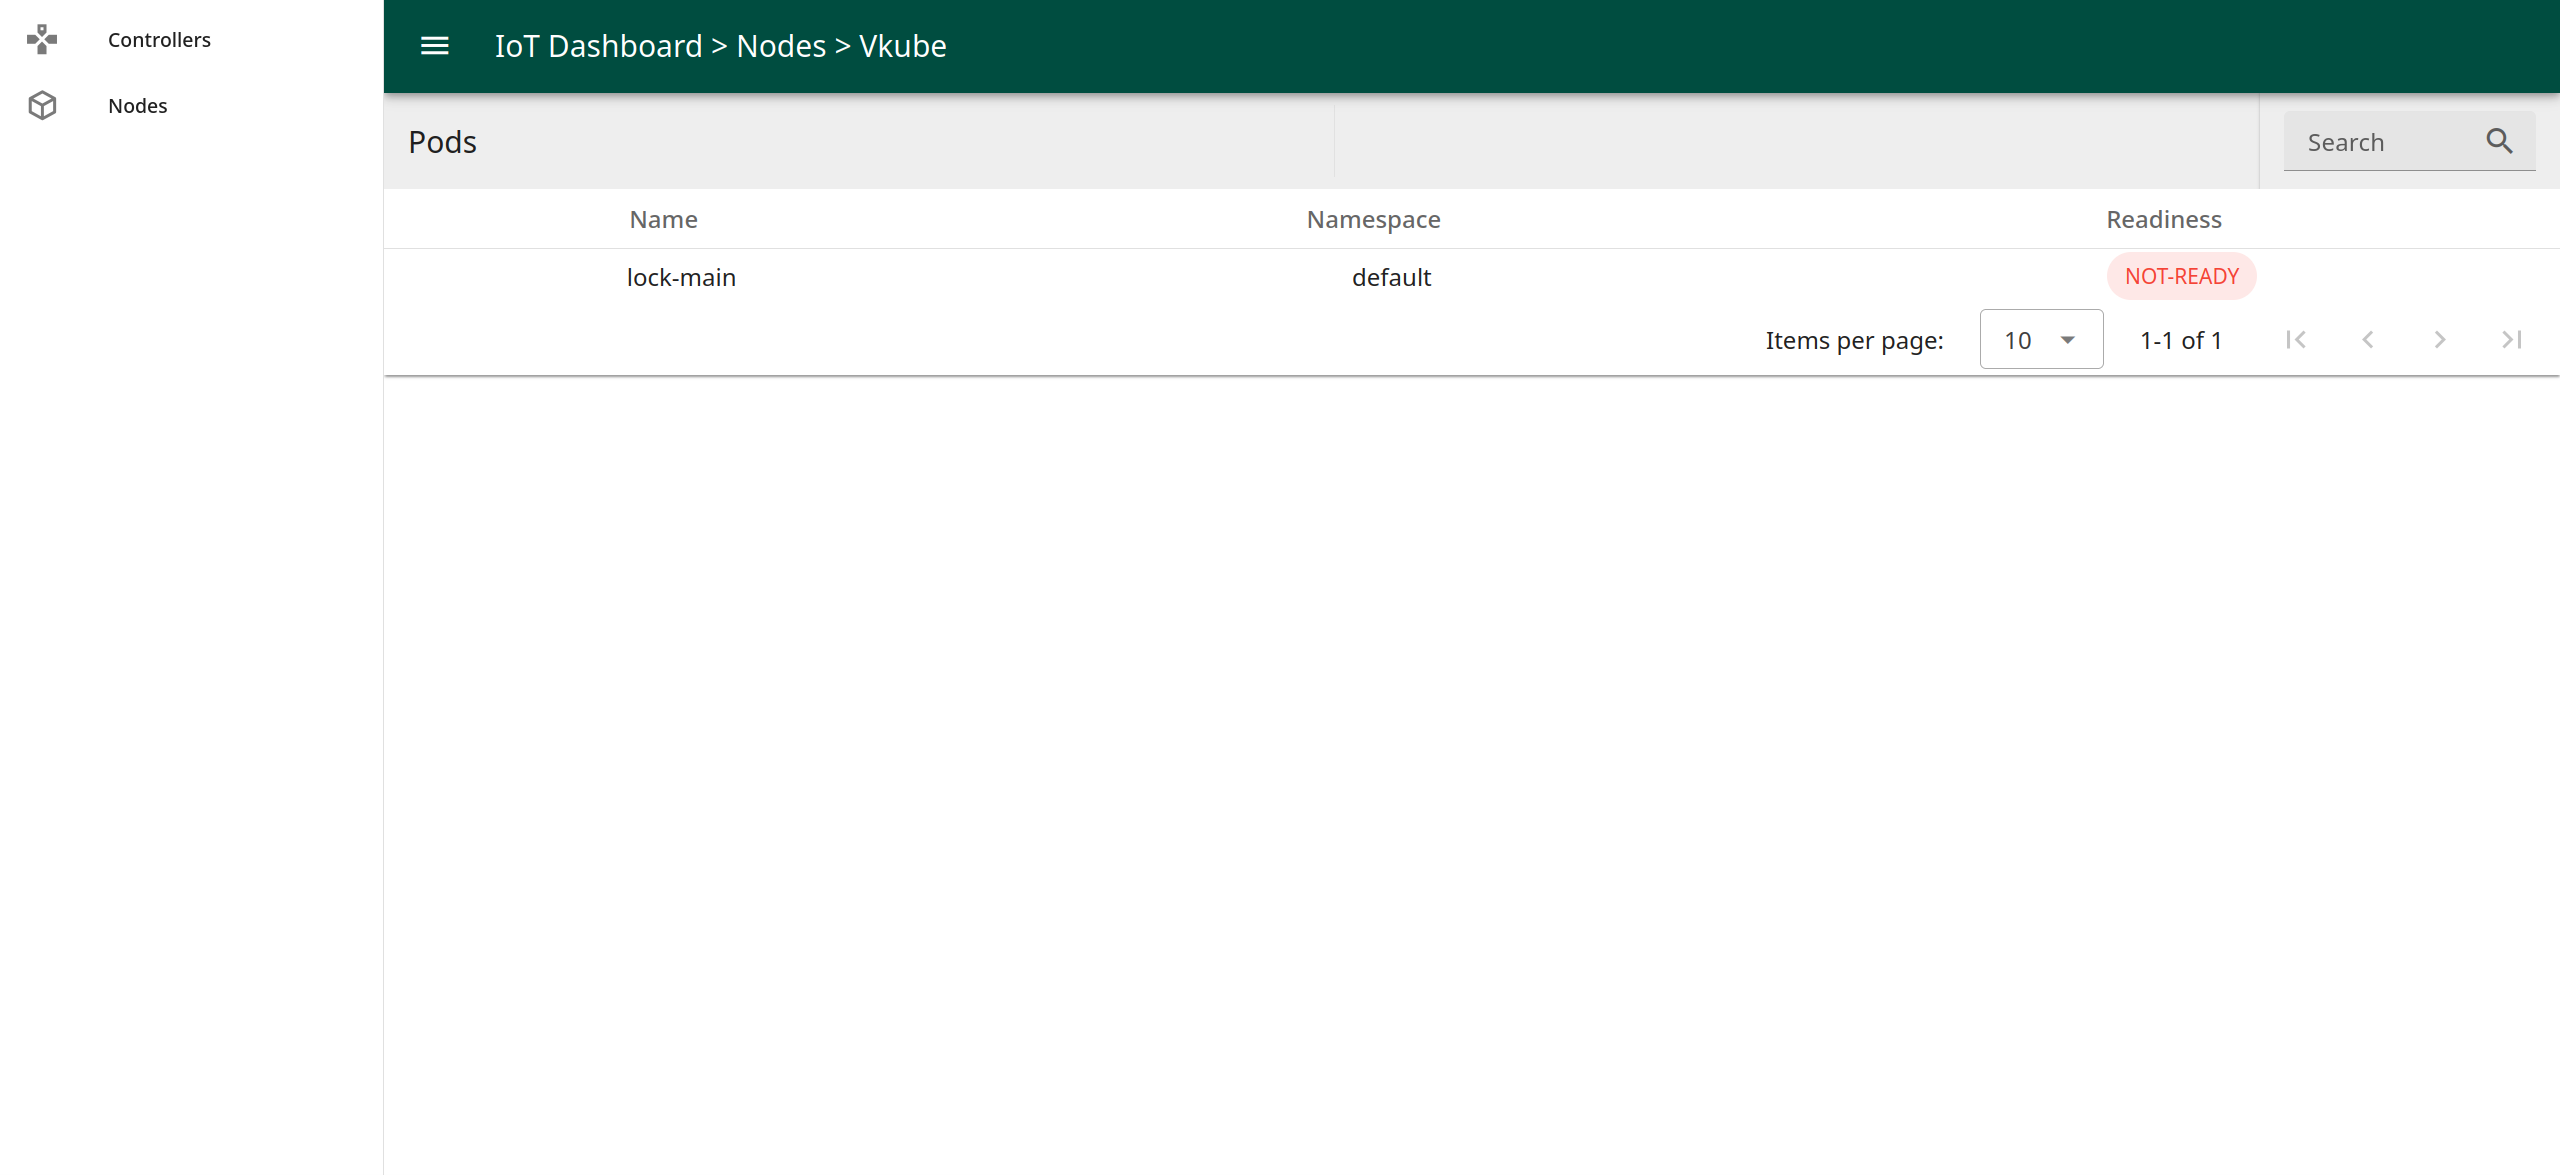
\includegraphics[width=\textwidth]{figs/dash_pod_lock_main_not_ready.png}}
        \caption{تغییر وضعیت پاد بدلیل تغییر وضعیت قفل مرکزی}
        \label{fig:dash_pod_lock_main_change readiness}
    \end{figure}
}

% \section{مقدمه}
% \paragraph{}{
%     هدف از این پژوهش انتشار روشی برای تولید پاسخ‌ها به صورت جمله است. برای این 
%     مورد، از شبکه‌های از پیش‌آموزش داده شده استفاده شده است. از 
%     \lr{LXMERT} \cite{tan-bansal-2019-lxmert}
%     به عنواان یک معماری دو‌جریان و از 
%     \lr{VisualBERT} \cite{li-etal-2020-bert-vision}
%     به عنوان یک معماری تک‌جریان بهره‌برداری شده است. 
% }


% % \vspace{15pt}

% \section{
%   معماری سیستم
%  }
% \paragraph{}{
%     برای حل این مسسله از معماری کدگذار-کدگشا استفاده شده‌است به گونه‌ای 
%     که از یک شبکه از پیش آموزش داده‌شده به عنوان کدگذار و از معماری‌های متفاوتی 
%     به عنوان کدگشا استفاده شده است. 
    
% }

% % \newpage

% % \vspace*{20pt}


% \begin{figure}[H]
%     % \center{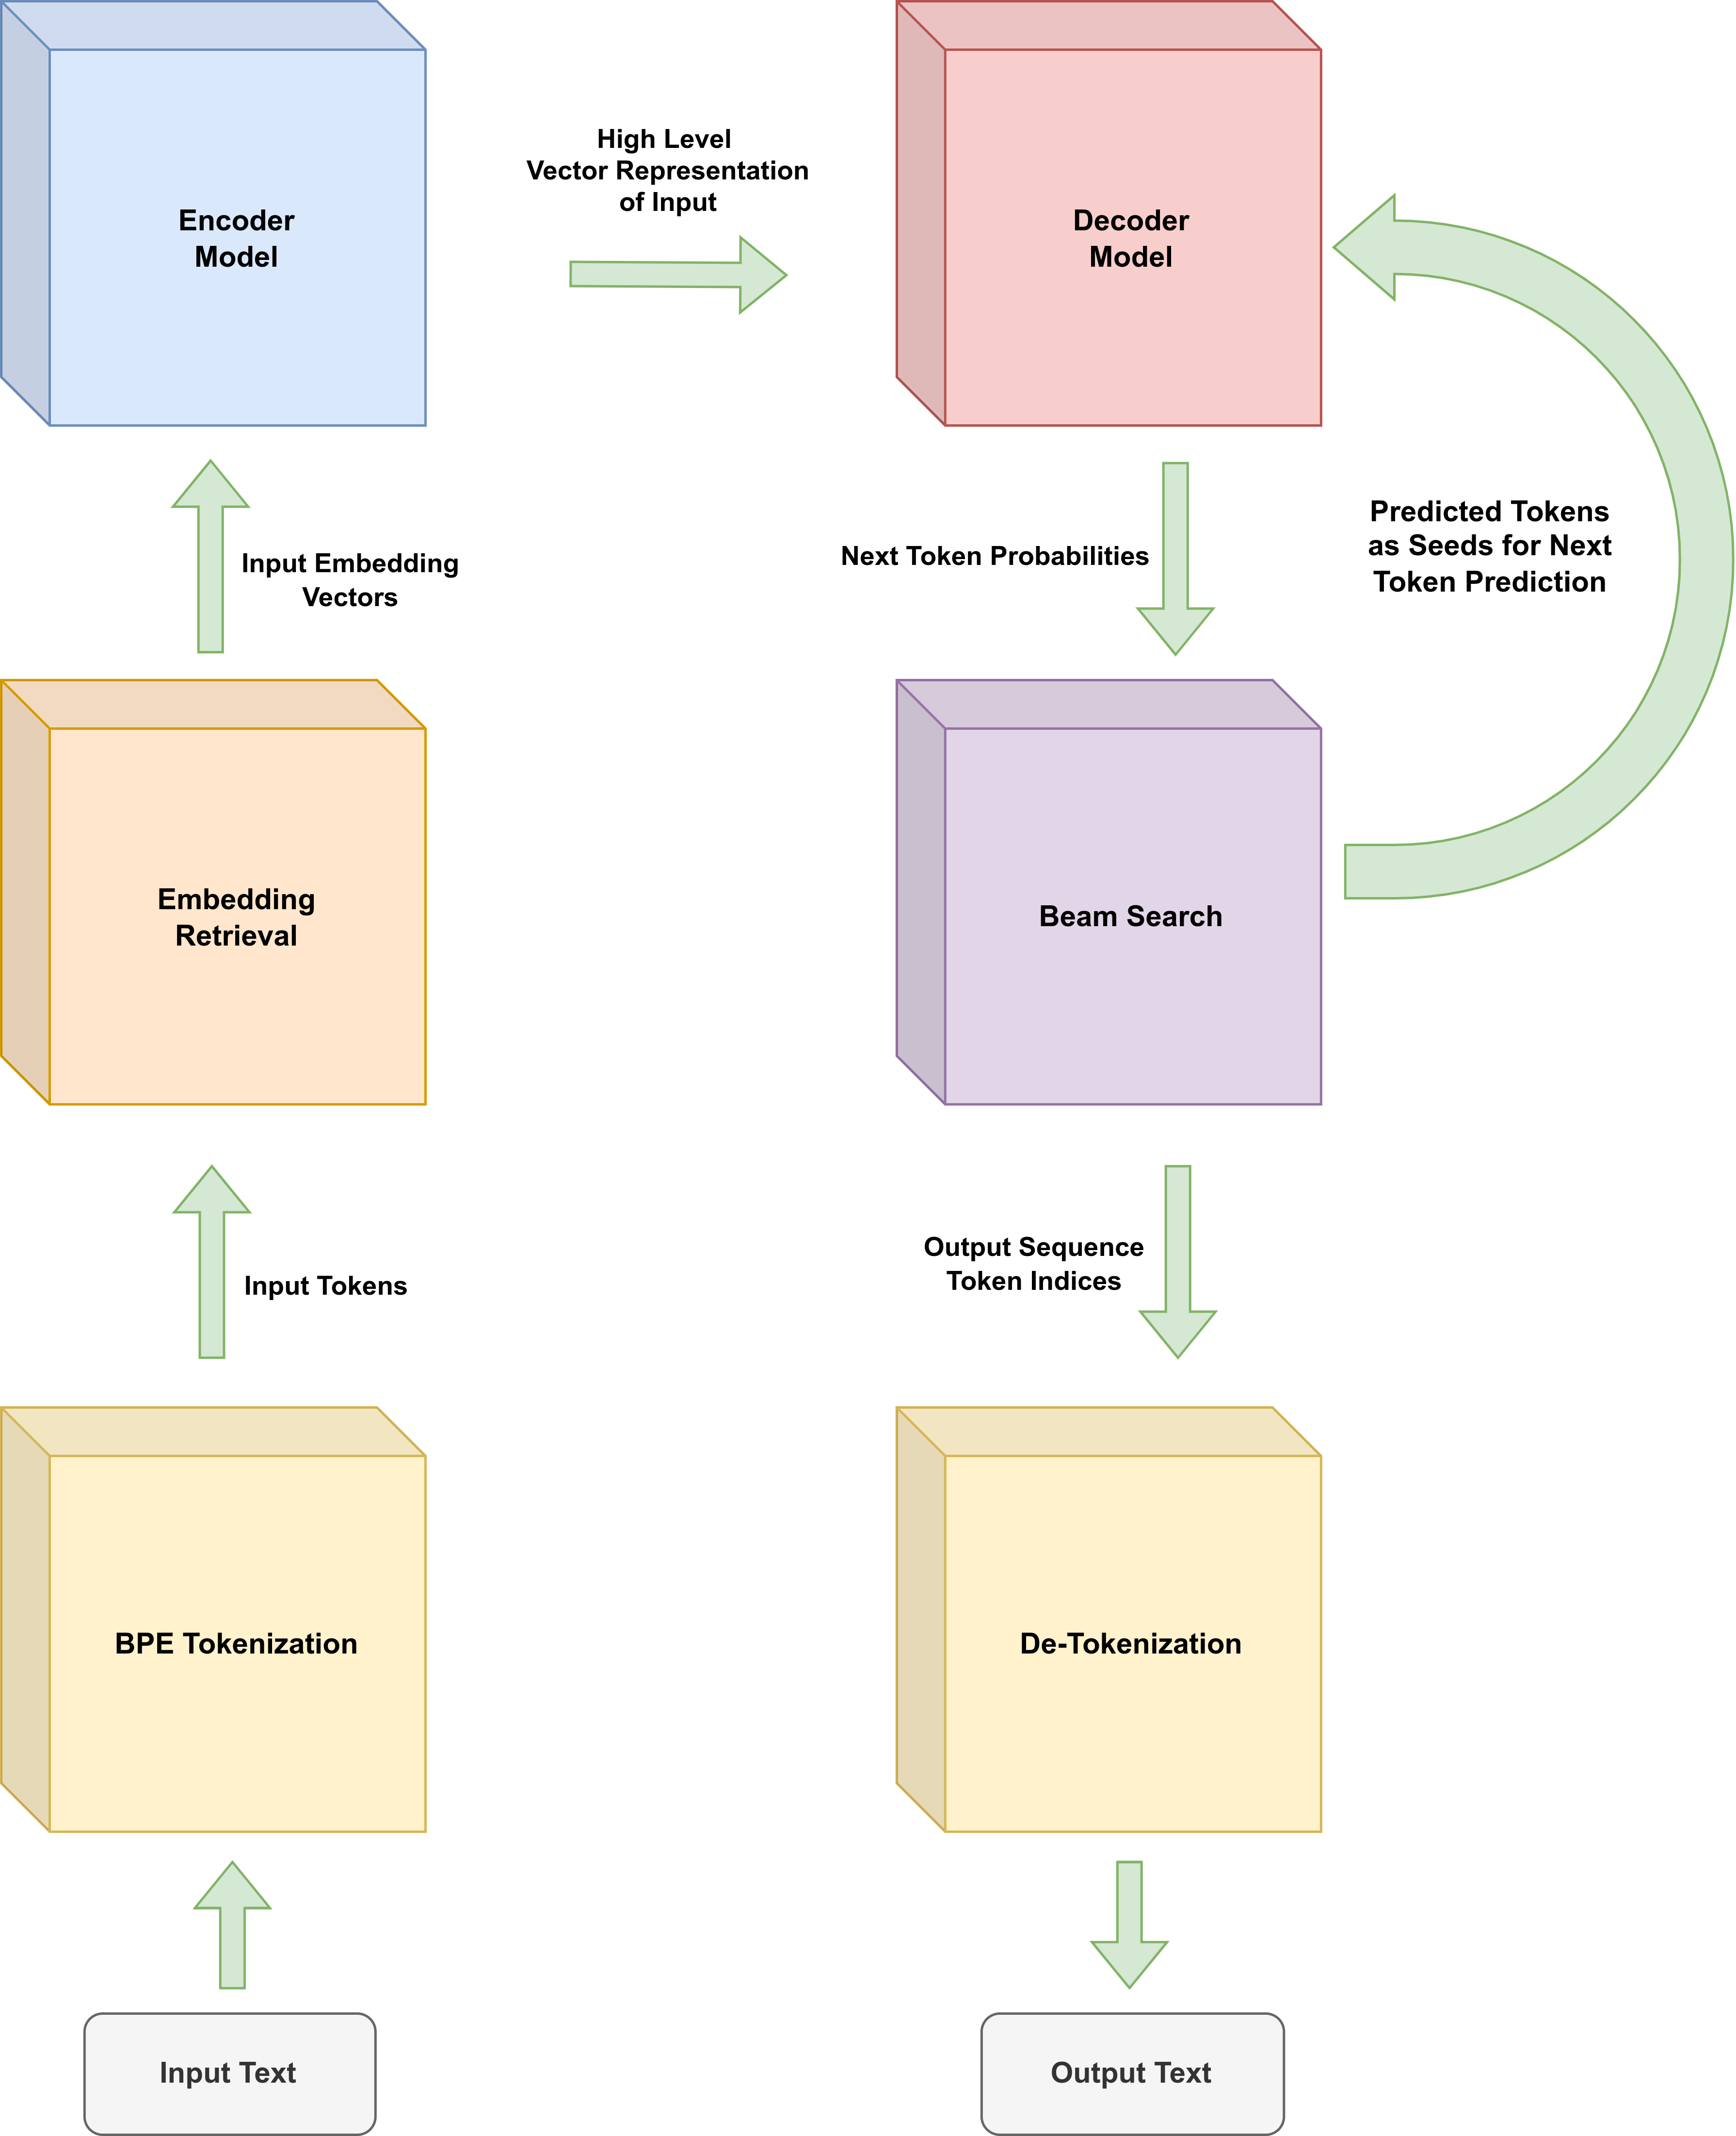
\includegraphics[width=1\textwidth]{figs/overview.png}}
%     \center{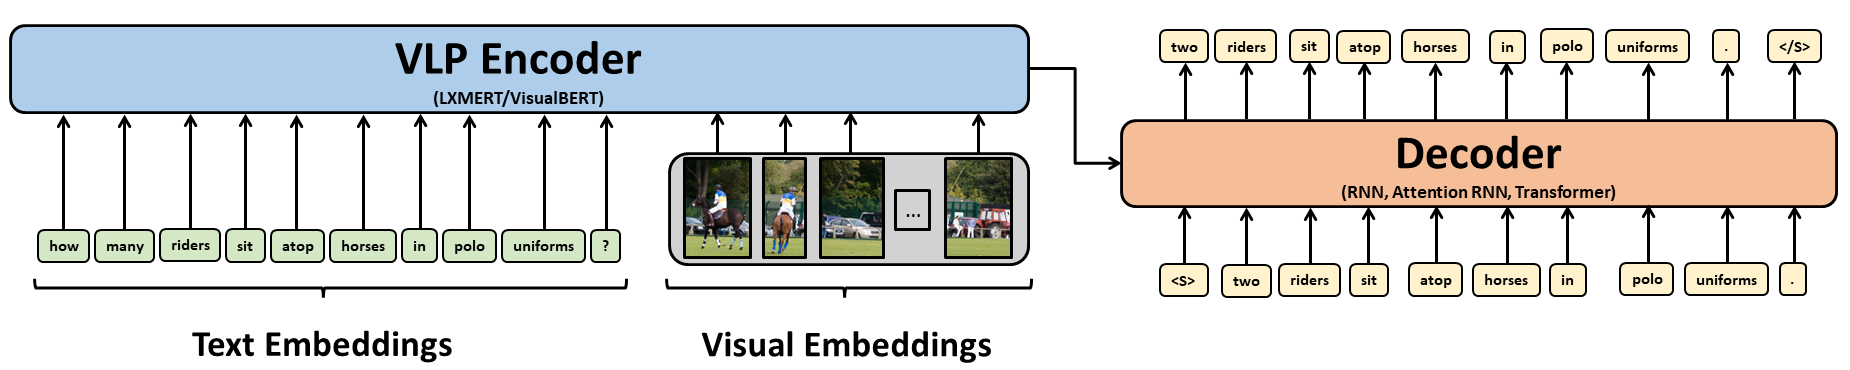
\includegraphics[width=1\textwidth]{figs/model architecture.png}}
%     \caption{شمای کلی سیستم پرسش‌و‌پاسخ تصویری}
%     \label{fig:overview}
% \end{figure}

% \newpage

% \section{
%   ورودی اولیه و خروجی نهایی
%  }

% \paragraph{}{
%     در ورودی سیستم باید بتوانیم تصویر و متن را به سیستم ورودی بدهیم. برای 
%     انجام این عمل باید هر دو بخش متن  و تصاویر را به بردار‌های ویژگی تبدیل کنیم. 
    
%     \begin{enumerate}
%         \item \textbf{بردارهای متن:}
%                 برای پردازش دقیق پرسش‌ها، لازم است که پرسش‌ها را به 
%                 بخش ‌های کوچک‌تری تقسیم کنیم که شبکه‌های عصبی عمیق قادر به اعمال محاسبات
%                 لازم باشند. به قسمت‌های کوچک‌تر اصطلاحا توکن گفته می‌شود. 
%                 به عمل جداسازی قمست‌های یک جمله 
%                 \lr{Tokenization}
%                 گفته می‌شود. عکس این عمل که همان اتصال توکن‌ها و تشکیل جمله است را
%                 \lr{De-Tokenization}
%                 نامیده می‌شود. در شکل 
%                 \ref{fig:tokenization}
%                 کارکرد این جداسازی مشاهده می‌شود. با توجه به اینکه هر دو شبکه
%                 \lr{LXMERT}
%                 و
%                 \lr{VisualBERT}
%                 بر پایه شبکه 
%                 \lr{BERT}
%                 هستند، برای بدست آوردن بردارهای ویژگی متن ورودی از جداساز 
%                 شبکه 
%                 \lr{BERT}
%                 استفاده شده‌است. 
%                 \begin{figure}[H]
%                     \center{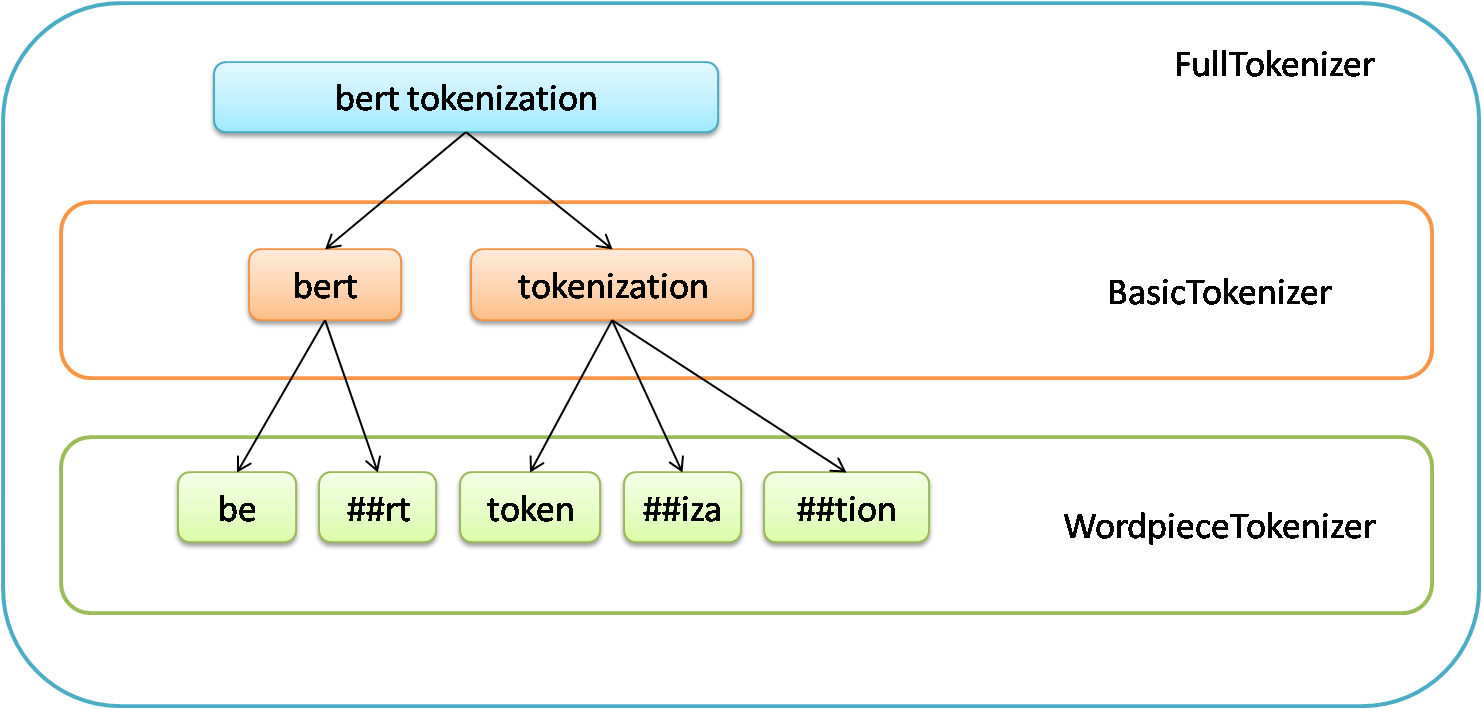
\includegraphics[width=0.8\textwidth]{figs/tokenization.png}}
%                     \caption{نمونه‌ای از کارکرد Tokenizer}
%                     \label{fig:tokenization}
%                 \end{figure}
%         \item  \textbf{بردارهای تصویر:}
%                 برای تبدیل تصاویر به بردارهای ویژگی مطابق با مقاله‌ای برای حل
%                 مسائل زبان-تصویر 
%                 \cite{anderson2018bottom}
%                 می‌توانیم هر تصویر را مجموعا به صورت 36 شیء در نظر بگیریم که از 
%                 شبکه عصبی
%                 \lr{Faster-RCNN} \cite{ren2015faster}
%                 تشخیص داده‌شده و هر شیء برداری با اندازه 2048 دارد.
                            
%     \end{enumerate}
% }

% \section {
%   مدل Encoder
%  }
% \paragraph{}{
%     از آنجایی که در بخش‌های قبل گفته شد، از مدل‌های از پیش آموزش داده‌شده 
%     استفاده می‌کنیم. به منظور مقایسه هر دو حالت تک‌جریان و دوجریان از دو مدل
%     تبدیل شونده با معماری‌های متفاوت استفاده شده است تا بتوان مقایسه جامع و
%     کاملی حول انواع مدل‌ها و عملکرد آن‌ها داشت. هدف از به کارگیری 
%     بخش کدگذار محاسبه یک بازنمایی از پرسش و تصویر همراه با یک‌دیگر و 
%     عبور دادن آن به بخش کدگشا است.
% }

% \subsection {
%   مدل LXMERT \cite{tan-bansal-2019-lxmert}
%  }
% \paragraph{}{
%     این مدل به عنوان یک مدل پایه برای حل مسئله پرسش و پاسخ تصویری ارائه شد. 
%     این مدل شامل سه بخش کدگذار تصویری، زبانی و میان‌ماژولی است. این مدل دو ورودی
%     می‌گیرد، یک تصویر و یک متن که همان پرسش مربوط به تصویر است. با 
%     ترتیب لایه‌های توجه به خود و توجه میانی باعث می‌شود که مدل بتواند 
%     یک بازنمایی از تصویر، یک بازنمایی از متن و یک بازنمایی 
%     میان‌ماژولی از ورودی‌ بدست بیاورد.  محققان در این مدل از روش‌های متفاوتی نظیر 
%     \lr{MLM} \footnote{\lr{Masked Language Modeling}}
%     ، MOP \footnote{\lr{Masked Object Prediction}}
%     و
%     تناظر میان‌ماژولی
%     \footnote{\lr{Cross-modality Matching}}
%     برای 
%     آموزش استفاده کرده‌اند که باعث شده است روابط درون‌ماژولی
%     و میان‌ماژولی به خوبی تشخیص داده شود. همانطوری که از تصویر 
%     \ref{fig:lxmert}
%     مشخص است این مدل یک مدل دوجریان است. 
%     \begin{figure}[H]
%         \center{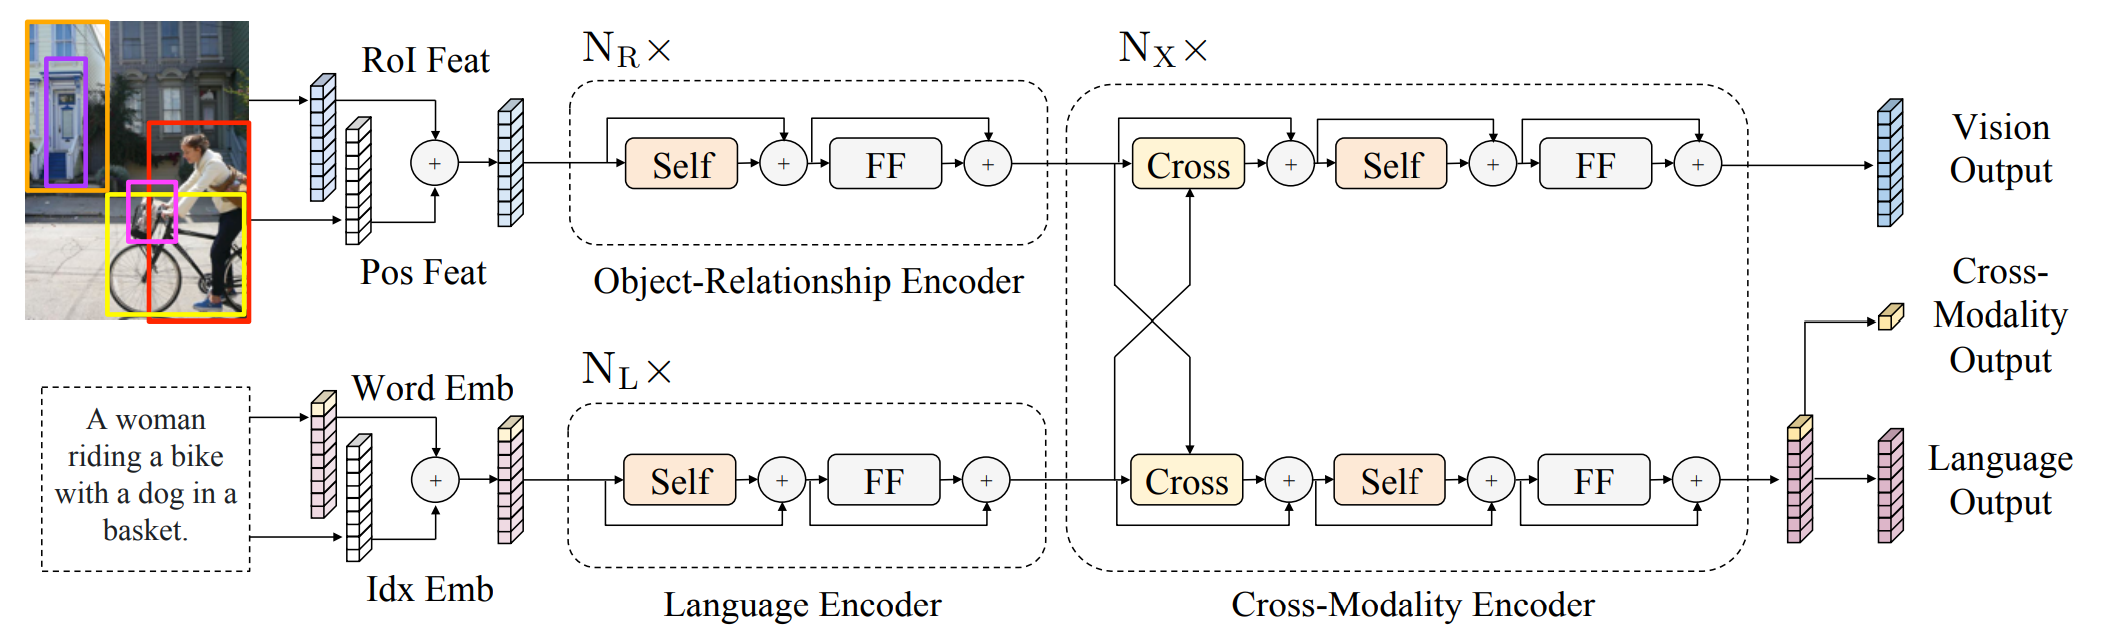
\includegraphics[width=1\textwidth]{figs/lxmert.png}}
%         \caption{معماری مدل LXMERT همراه با ورودی و خروجی}
%         \label{fig:lxmert}
%     \end{figure}
% }

% \subsection{
%     مدل VisualBERT \cite{li-etal-2020-bert-vision}
% }

% \paragraph{}{
%     پس از انتشار 
%     LXMERT
%     و پیشرفت چشمگیرش در حل مسئله پرسش‌وپاسخ تصویری پژوهش‌های بسیاری 
%     برای بهبود بیشتر انجام شد. از جمله این پژوهش‌ها بررسی مدل 
%     BERT
%     و عملکرد آن در مسائل زبان-تصویر را میتوان نام برد که منجر به انتشار مدل
%     VisualBERT \cite{li-etal-2020-bert-vision}
%     شد. این مدل به صورت تک‌جریان است و دنباله‌ای از بردار‌های ویژگی متن
%     همراه با دنباله‌ای از بردارهای ویژگی تصویر را ورودی می‌گیرد و خروجی را
%     به صورت بردارهای بازنمایی می‌دهد. به علاوه، میزان توجه 
%     بردار‌های ویژگی توکن‌ها و بردار‌های ویژگی اشیاء موجود در تصویر 
%     را با یکدیگر اندازه‌گیری کردند و اشیاء با توکن‌های مربوطه به‌خوبی
%     توجه خورده‌اند. برای مثال با توجه به شکل 
%     \ref{fig:visualbert}
%     در لایه 11 کلمه 
%     man
%     به خوبی با محدوده مربوط به مرد موجود در تصویر مرتبط شده است!
%     \begin{figure}[H]
%         \center{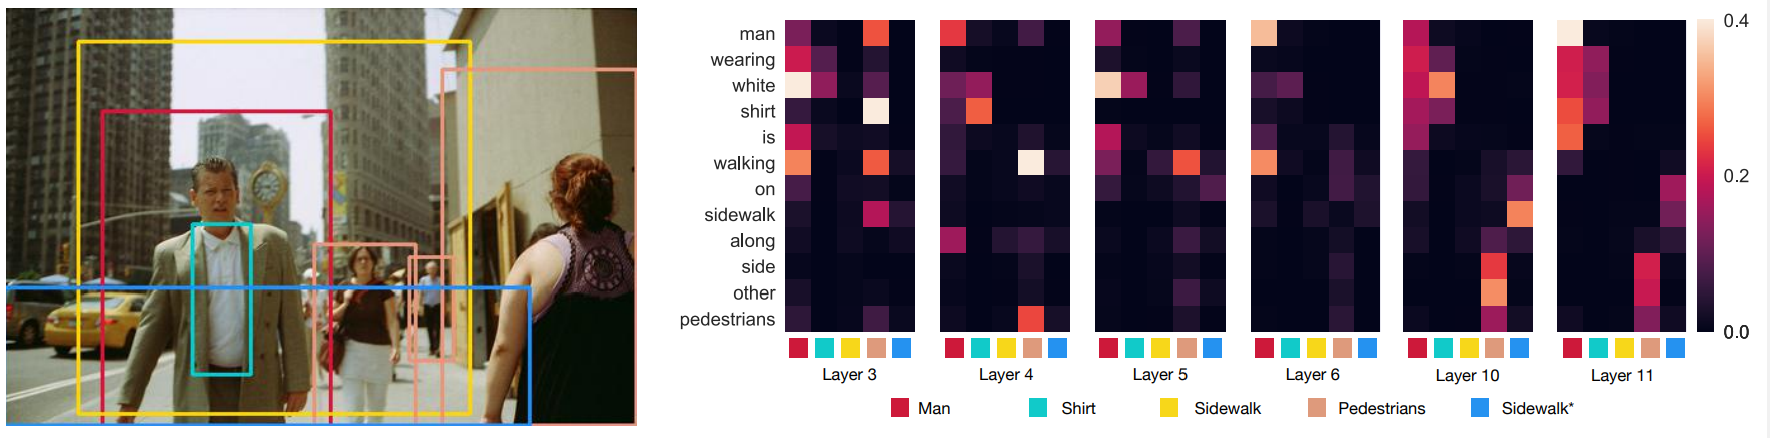
\includegraphics[width=1\textwidth]{figs/VisualBERT.png}}
%         \caption{میزان توجه بخش متن به تصاویر در VisualBERT}
%         \label{fig:visualbert}
%     \end{figure}
% }

% \section{
%   مدل Decoder
%  }
% \paragraph{}{
%     پس از آنکه بردارهای بازنمایی تصویر و پرسش توسط کدگذار محاسبه شد، لازم
%     است که أن‌ها را برای تولید پاسخ به بخش کدگشا بدهیم. 
%     بخش کدگشای معماری‌های ارائه شده از دو معماری شبکه‌های عصبی بازگشتی و 
%     شبکه‌های تبدیل‌شونده استفاده شده است. برای تولید پاسخ از مکانیزم
%     Autoregressive 
%     استفاده شده است. در این مکانیزم توکن‌ها بر اساس توکن‌های قبلی پیش‌بینی می‌شوند
%     و سپس همان توکن جدید همرا با دنباله قبلی برای توکن جدید دیگری مطابق با
%     شکل 
%     \ref{fig:decoder}
%     به کدگشا 
%     ورودی داده می‌شوند. 
%     \begin{figure}[H]
%         \center{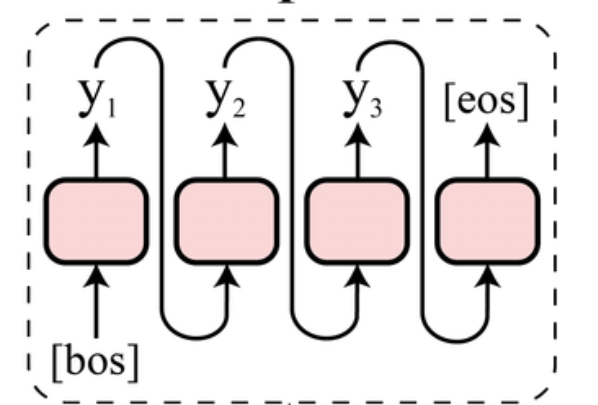
\includegraphics[scale=1]{figs/Autoregressive.png}}
%         \caption{ساختار مدل \lr{Autoregressive Decoder}}
%         \label{fig:decoder}
%     \end{figure}
% }

% \section{جمع‌بندی}
% \paragraph{}{
%     در این بخش از نوشتار به بررسی دقیق اجزای تشکیل‌دهنده‌ی سیستم پیشنهادی برای
%     حل مسا‌له‌ی پرسش‌وپاسخ تصویری پرداختیم.
%     روشی نو برای حل این‌ مسئله که باعث رفع ابهامات بسیاری می‌شود. اشاره شد که
%     از مدل‌های از پیش آموزش داده‌شده استفاده کردیم و همچنین برای 
%     مقایسه نتایج و بدست آوردن بهترین معماری، چندین حالت بررسی شد که در 
%     بخش
%     \ref{ch:eval}
%     به مقایسه نتایح پرداخته‌ خواهد شد.
% }
% !TeX root=main.tex

\chapter{ارزیابی روش پیشنهادی} \label{ch:eval}
\thispagestyle{empty}


\section{مقدمه}
\paragraph{}{
    در این فصل برای بررسی عملکرد روش پیشنهادی در فصل قبل، سیستم مورد نظر به طور کامل پیاده‌سازی
    شده و بر روی یک مجموعه‌داده‌ی شناخته‌شده اجرا شده است.
    برای ارزیابی روش پیشنهادی روش‌های متفاوتی ارائه شده است. 

    برای انتخاب رویکرد مناسب ارزیابی از میان خیل عظیمی از روش‌های شناخته‌شده
    عوامل متعددی مورد بررسی قرار می‌گیرد و با توجه به آن‌ها یک یا چند روش انتخاب می‌شود.
    مهم‌ترین عامل ساختار و جنس داده‌های خروجی مدل و همچنین جنس داده‌های ارزیابی است. باتوجه به مدل و مجموعه
    داده‌ مورد استفاده، در این پژوهش نیاز به معیارهای ارزیابی برای مقایسه جملات داریم. 
    از آنجایی که این روش، روشی نو است برای اثبات درستی آن از معیار‌های ارزیابی متفاوتی استفاده کردیم 
    که به طور کلی در دو بخش دسته‌بندی می‌شود. 
}

% \section{
%     معیارهای برپایه شباهت نحوی
% }
% \label{sec:wordbased}
% \paragraph{}{
%     معیارهای برپایه شباهت نحوی به یکسان بودن توکن‌ها در
%     یک جمله تمرکز دارد. به عبارتی براساس تعداد توکن‌های 
%     انتخابی و برابری آن‌ها امتیازی بین دو جمله در نظر گرفته
%     شده که نشانگر میزان شباهت دو جمله به یکدیگر است. 
%     در این پژوهش از معیارهای 
%     BLEU \cite{papineni2002bleu}،
%     Rouge \cite{lin2004rouge}،
%     و
%     METEOR \cite{banerjee2005meteor}
%     به عنوان معیارهای شباهت بر پایه توکن‌ها استفاده‌ شده است.
%     این معیارها معمولا برای ترجمه‌های ماشینی استفاده می‌شوند و از آنجایی
%     که هدف مقایسه دو جمله پاسخ و جمله مرجع است 
%     استفاده از این معیارها برای سنجش سیستم راه حل مناسبی است.

% }

% \section{
%   معیارهای برپایه بردارهای تعبیه
% } \label{sec:embeddingbased}
% \paragraph{}{
%     در این معیارها با بهره‌برداری از بردارهای تعبیه
%     \footnote{\lr{Embedding vectors}}
%     به محاسبه شباهت بین جملات پرداخته می‌شود. 
%     در این پژوهش از دو معیار
%     BERTScore \cite{zhang2019bertscore}
%     و 
%     \lr{Average Score}
%     به عنوان معیارهای بردار تعبیه استفاده شده است.
% }

% \subsection{
%   معیار BERTScore \cite{zhang2019bertscore}
% } \label{subsec:BERTScore}
% % \vspace*{10pt}
% \paragraph{}{
%     BERTScore 
%     یک معیار ارزیابی خودکار است که برای ارزیابی 
%     سیستم‌های تولید متن استفاده می‌شود.
%     برخلاف روش‌های رایج موجود که شباهت 
%     نحوی توکن‌ها را محاسبه می‌کنند، 
%     BERTScore 
%     بر محاسبه شباهت معنایی بین توکن‌های مرجع و
%     توکن‌های پیش‌بینی شده تمرکز دارد. 
%     نویسنده مقاله آن را بر روی ترجمه‌های ماشینی و 
%     وظایف توضیح تصاویر آزمایش کرد و 
%     دریافت که با قضاوت های انسانی ارتباط بهتری دارد.

%     از مزایای این معیار نسبت به مقایسه نحوی می‌توان به عدم محاسبه 
%     توکن‌های هم‌معنی در نظر گرفت. برای مثال معیارهای برمبنای شباهت نحوی، 
%     درصورت مغایرت توکن‌ها هیچ امتیازی در نظر نمی‌گیرند در حالی که
%     BERTScore
%     به نزدیکی معانی کلمات توجه می‌کند.
% }

% \subsection{
%     معیار 
%     Score Average
% } \label{subsec:average-score}
%     % \vspace*{10pt}
% \paragraph{}{
%     برای محاسبه این معیار، در ابتدا یک میانگین از بردارهای تعبیه جملات گرفته 
%     و سپس با استفاده از تابع شباهت کسینوسی میزان شباهت بین جملات مرجع و جملات
%     پیش‌بینی شده محاسبه می‌شود.
%     (معادله \ref{eq:avg-score-sim})
%     \begin{equation}
%         \label{eq:avg-score}
%         Score(s = [t_1, t_2, ..., t_T]) = \frac{1}{T}\sum_{i=0}^{T}{Embedding(t_i)}
%     \end{equation}

%     \begin{equation}
%         \label{eq:avg-score-sim}
%         sim(s_1, s_2) = \frac{\vec{Score(s_1)}.\vec{Score(s_2)}}{||Score(s_1)||\times||Score(s_2)||} 
%     \end{equation}
% }


% \section{
%   مجموعه‌داده‌ی مورد استفاده
%  }
%  \label{sec:dset}
% \paragraph{}{
%     در بخش 
%     \ref{sec:vqa_datasets}
%     به معرفی بخش اعظمی از مجموعه‌ داده‌های موجود
%     در پرسش‌وپاسخ تصویری پرداخته‌شد. با این حال اگر
%     به این مجموعه‌ داده‌ها با دید عمیق تری بنگریم متوجه این
%     موضوع می‌شویم که در هیج‌کدام از این مجموعه‌ها پاسخ‌ها
%     به صورت جمله کامل نیستند، به عبارتی برای 
%     حل آن‌ها استفاده از دسته‌بندی کافی است. برای ارزیابی دقیق
%     سیستم پیشنهادی نیازمندی مجموعه داده‌ای است که پاسخ‌های 
%     پرسش‌ها به صورت جمله باشد. 
%     مجموعه داده 
%     \lr{Full Sentence Visual Question Asnwering (FSVQA)}
%     \cite{shin2016color}
%     این خاصیت را دارد و بهترین گزینه برای استفاده به عنوان 
%     مجموعه داده ارزابی است. 

%     مجموعه داده FSVQA 
%     شامل یک تصویر و یک پرسش مربوط به آن است 
%     و جمله یه صورت پاسخ آن پرسش به عنوان
%     هدف در نظر گرفته شده است. 
%     این پاسخ‌ها از دو مجموعه داده 
%     VQA \cite{VQA}
%     و 
%     MSCOCO \cite{caesar2018coco}
%     و بر اساس قوانین زبان 
%     انگلیسی به صورت خودکار تولید شده‌اند. 
%     توجه به این نکته حائز اهمیت است که تولید جملات از 
%     این روش امکان 
%     ایجاد اشکالاتی را در مجموعه داده بوجود می‌آورد 
%     و مدل‌ها نیز قادر به یادگیری الگوی پاسخ‌ها
%     یا همان قوانین هستند. 

% }

% \section{
%   نتایج ارزیابی سیستم پیشنهادی
%  }
%  \label{sec:eval}
% \paragraph{}{
%     براساس توضیحات‌ داده‌شده سیستم پیشنهادی را با معماری‌های
%     متفاوت پیاده‌سازی و برروی مجموعه داده معرفی شده در بخش 
%     \ref{sec:dset}
%     آموزش دادیم.
%     سپس هر کدام از معماری‌ها برروی داده‌ ارزیابی
%     سنجیده شد. علاوه بر سنجش مدل‌ها و معماری‌های متفاوت
%     میزان تاصیر تغییرات در هر معماری نیز مورد مطالعه
%     قرار گرفته‌‌شده‌ است. 
% }

% \subsection{ارزیابی و مقایسه معماری‌های ارجح}
% \paragraph{}{
%     پس از بدست آوردن نتایج،‌ به مقایسه معماری‌های مورد استفاده پرداخته‌شده است. 
%     با توجه به جدول
%     \ref{table1}
%     همان‌طوری که انتظار می رفت، شبکه‌های عصبی 
%     Transformers
%     همراه با شبکه LXMERT
%     به عنوان کدگذار بهترین عملکرد را داشت. اگر اندکی نتایج را وارسی کنیم
%     متوجه بالا بودن امتیازها می‌شویم که 
%     نسبت به مدل‌های مشابه در توضیح تصاویر مقادیر بسیار بالایی دارند. مطابق با آنچه در بخش
%     \ref{sec:dset}
%     بحث شد، یکی از دلایل را می‌توان ساده‌ بودن مجموعه داده در نظر گرفت. از آنجایی 
%     که مجموعه داده از قوانین از پیش تعیین شده و بصورت خودکار تولید شده‌اند، مدل‌ها 
%     و به خصوص کدگشا ممکن است این الگوها را آموزش دیده باشند. با این حال در 
%     همه حالات از دقتی که نویسندگان مجموعه داده گزارش کرده‌ بودند عملکرد بهتری داشته‌ایم. 
    
%     \begin{table}[h]
%         \centering
%         \tiny
%         \resizebox{\textwidth}{!}{
%         \begin{tabular}{llccccccc}
%             \hline
%             \multicolumn{2}{l}{Method} &  & \multicolumn{3}{c}{Word-based} &  & \multicolumn{2}{c}{Embedding-based}\\ 
%             \cline{0-1} \cline{4-6} \cline{8-9}
%             Encoder & Decoder & & BLEU & METEOR & ROUGE-L& & \lr{Average Score} & \lr{BERT Score} \\
%             \hline
%             \lr{LSTM Q+I} & \lr{LSTM} & & \lr{23.9} & \lr{23.3} & - &  & - & - \\
%             \hline
%             \multirow{7}{*}{LXMERT} 
%             & \lr{1-LSTM} & & \lr{32.19} & \lr{56.65} & \lr{56.38} & & \lr{86.50} & \lr{79.19} \\
%             & \lr{1-GRU} & & \lr{39.37} & \lr{62.99} & \lr{61.50} & & \lr{89.63} & \lr{82.07} \\
%              \cline{2-3}
%              & \lr{1-LSTM+Bahdanau attention} & & \lr{79.03} & \lr{86.43} & \lr{85.49} & & \lr{95.94} & \lr{91.84} \\
%              & \lr{1-LSTM+Luong(general) attention} & & \lr{79.54} & \lr{86.96} & \lr{86.25} &  & \underline{\lr{96.11}} & \lr{91.90} \\
%               & \lr{1-GRU+Bahdanau attention} & & \lr{71.40} & \lr{83.26} & \lr{82.62} &  & \lr{95.42} & \lr{89.32} \\
%               & \lr{1-GRU+Luong(dot) attention} & & \lr{73.92} & \lr{84.71} & \lr{83.84} &  & \lr{95.73} & \lr{90.37} \\
%              \cline{2-3}
%              & \lr{3-Transformer Decoder} & & \textbf{\underline{\lr{86.73}}} & \textbf{ \underline{\lr{91.18}}} & \textbf{\underline{\lr{90.60}}} &  & \lr{90.20} & \textbf{\underline{\lr{95.01}}} \\
%             \hline
%             \multirow{7}{*}{\lr{VisualBERT}} & \lr{1-LSTM} & & \lr{18.62} & \lr{38.00} & \lr{38.35} &  & \lr{84.83} & \lr{69.20} \\
%             & \lr{1-GRU} & & \lr{22.51} & \lr{44.24} & \lr{43.72} &  & \lr{87.74} & \lr{73.59}\\
%              \cline{2-3}
%              & \lr{1-LSTM+Bahdanau attention} & & \lr{84.27} & \lr{88.07} & \lr{87.28} &  & \lr{97.11} & \lr{93.50}\\
%              & \lr{1-LSTM+Luong(concat) attention} & & \lr{82.90} & \lr{87.71} & \lr{86.90} &  & \textbf{\underline{\lr{97.17}}} & \lr{93.11}\\
%              & \lr{1-GRU+Bahdanau attention}& & \lr{72.20} & \lr{82.87} & \lr{82.40} &  & \lr{96.10} & \lr{89.26}\\
%              & \lr{1-GRU+Luong(dot) attention} & & \lr{79.65} & \lr{86.17} & \lr{85.23} &  & \lr{96.93} & \lr{91.81}\\
%               \cline{2-3}
%             & \lr{3-Transformer Decoder} & & \underline{\lr{85.95}} & \underline{\lr{89.76}} & \underline{\lr{89.09}} &  & \lr{91.94} & \underline{\lr{94.44}} \\
%             \hline
%         \end{tabular}
%         }
%         \caption{نتایج معماری‌های متفاوت بر مجموعه داده \lr{FSVQA}.
%                 اعداد موجود در نام کدگشا نشانگر تعداد لایه‌های آن است. }
%         \label{table1}
%         % \vspace{-2mm}    
%     \end{table}
    
% }

% \subsection{مقایسه شبکه‌های عصبی بازگشتی}
% \label{subsec:analysis-rnn}
% \paragraph{}{
%     در این بخش به بررسی تغییرات کدگشا‌های بر پایه شبکه‌های 
%     عصبی بازگشتی پرداخته‌شده است. برای بررسی بیشتر تعداد لایه‌های شبکه
%     و نوع شبکه‌ها و همچنین جهت جریان اطلاعات در شبکه‌ها مورد بررسی قرار گگرفت که نتایج
%     با تمام جزئیات در جدول 
%     \ref{table2}
%     آورده شده‌اند. با توجه به این جدول می‌توانیم نتیجه بگیریم که برترین معماری
%     مربوط به استفاده از 3 لایه شبکه‌های LSTM
%     به صورت دو طرفه است. اگر به نتایج کدگذار‌ها دقت کنیم متوجه می‌شویم که استفاده از 
%     VisualBERT
%     به عنوان کدگذار در این حالت به خوبی 
%     LXMERT
%     عمل نمی‌کند. در حالت کلی این معماری برا حل مسئله به روش و با توجه وجود معماری‌های نوین،
%     استفاده از این معماری پیشنهاد نمی‌شود. 

%     \begin{table}[ht!]
%         \centering
%         \resizebox{\textwidth}{!}{
%         \begin{tabular}{llccccccc}
%             \hline
%             \multicolumn{2}{l}{Method} &  & \multicolumn{3}{c}{Word-based} &  & \multicolumn{2}{c}{Embedding-based}\\ 
%             \cline{0-1} \cline{4-6} \cline{8-9}
%             Encoder & Decoder & & BLEU & METEOR & ROUGE-L & & \lr{Average Score} & \lr{BERT Score} \\
%             \hline
%             \multirow{12}{*}{LXMERT} & \lr{1-LSTM} & & \lr{32.19} & \lr{56.65} & \lr{56.38} & & \lr{86.50} & \lr{79.19}\\
%              & \lr{2-LSTM} & & \lr{41.28} & \lr{64.39} & \lr{62.97} & & \lr{89.57} & \lr{83.10} \\
%              & \lr{3-LSTM} & & \lr{41.10} & \lr{64.25} & \lr{63.02} &  & \lr{89.54} & \lr{82.67}\\
%              & \lr{1-GRU} & & \lr{39.37} & \lr{62.99} & \lr{61.50} & & \lr{89.63} & \lr{82.07} \\
%              & \lr{2-GRU} & & \lr{35.23} & \lr{59.57} & \lr{58.24} &  & \lr{88.56} & \lr{79.68} \\
%              %& 3-GRU & & running & running & running & & running & running \\
%              &  \lr{1-BiLSTM} & & \lr{41.97} & \lr{65.25} & \lr{63.65} &  & \lr{90.11} & \lr{83.51}\\
%              & \lr{2-BiLSTM} & & \lr{43.26} & \lr{66.28} & \lr{64.67} &  & \lr{90.47} & \textbf{\underline{\lr{84.09}}}\\
%              & \lr{3-BiLSTM} & & \textbf{\underline{\lr{43.54}}} & \textbf{\underline{\lr{66.39}}} & \textbf{\underline{\lr{64.74}}} &  & \textbf{\underline{\lr{90.58}}} & \lr{84.02} \\
%              & \lr{1-BiGRU} & & \lr{40.89} & \lr{64.15} & \lr{62.66} &  & \lr{89.88} & \lr{82.46}\\
%              & \lr{2-BiGRU} & & \lr{34.32} & \lr{58.54} & \lr{57.29} &  & \lr{88.74} & \lr{79.27}\\
%              & \lr{3-BiGRU} & & \lr{27.88} & \lr{54.82} & \lr{54.55} &  & \lr{86.66} & \lr{74.72}\\
%             \hline
%             \multirow{12}{*}{VisualBERT} & \lr{1-LSTM} & & \lr{18.62} & \lr{38.00} & \lr{38.35} &  & \lr{84.83} & \lr{69.20} \\
%              & \lr{2-LSTM} & & \lr{18.92} & \lr{38.62} & \lr{38.42} &  & \lr{85.30} & \lr{70.40}\\
%              & \lr{3-LSTM} & & \lr{19.30} & \lr{39.33} & \lr{38.80} &  & \lr{85.87} & \lr{71.35}\\
%              & \lr{1-GRU} & & \lr{22.51} & \lr{44.24} & \lr{43.72} &  & \lr{87.74} & \lr{73.59}\\
%              & \lr{2-GRU} & & \lr{21.96} & \lr{45.16} & \lr{44.93} &  & \lr{88.21} & \lr{73.26} \\
%              & \lr{3-GRU} & & \lr{11.36} & \lr{32.34} & \lr{33.99} &  & \lr{84.23} & \lr{67.15}\\
%              &  \lr{1-BiLSTM} & & \lr{20.03} & \lr{39.70} & \lr{39.75} &  & \lr{85.52} & \lr{71.19}\\
%              & \lr{2-BiLSTM} & & \lr{18.84} & \lr{40.05} & \lr{40.27} &  & \lr{86.67} & \lr{72.13}\\
%              & \lr{3-BiLSTM} & & \lr{20.46} & \lr{41.51} & \lr{41.19} &  & \lr{87.21} & \lr{73.43}\\
%              & \lr{1-BiGRU} & & \underline{\lr{22.72}} & \underline{\lr{45.66}} & \underline{\lr{45.26}} &  & \underline{\lr{88.42}} & \underline{\lr{74.32}}\\
%              & \lr{2-BiGRU} & & \lr{19.70} & \lr{42.21} & \lr{41.84} &  & \lr{88.04} & \lr{73.33}\\
%              & \lr{3-BiGRU} & & \lr{15.76} & \lr{36.74} & \lr{36.37} &  & \lr{85.93} & \lr{69.14} \\
%             \hline
%         \end{tabular}
%         }
%         \caption{تاثیر معماری‌های متفاوت در کدگشاهای بر پایه شبکه‌های عصبی بازگشتی}
%         \label{table2}
%         % \vspace{-2mm}    
%     \end{table}
% }

% \subsection{ارزیابی و مقایسه شبکه‌های عصبی بازگشتی و مکانیزم توجه سراسری}
% \paragraph{}{
%     بررسی نتایج بخش 
%     \ref{subsec:analysis-rnn}
%     نشان داد که استفاده از شبکه‌های عصبی بازگشتی به تنهایی پاسخگوی نیازهای مجموعه داده
%     مورد نظر نیست. برای رفع این مشکل از مکانیزم‌های توجه سراسری نظیر باهدانا و لوآنگ که
%     در بخش 
%     \ref{subsec:bahdanau_attn}
%     و
%     بخش
%     \ref{subsec:loung}
%     توضیح داده شده‌اند استفاده کرده و از هر سه متد 
%     الحاق، جمع و ضرب آن‌ها را مورد بررسی قرار داده‌شده است. بررسی نتایحج مشخص می‌کند که استفاده
%     از این مکانیزم کمک بسیاری به شبکه کرده و امتیازهای نحوی و معنایی هر دو به خد قابل توجهی
%     بالا رفته‌اند. از نتایج این بخش می‌توان نتیجه گرفت استفاده از شبکه کدگذار
%     VisualBERT
%     عمکرد بهتری دارد و پیشنهاد می‌شود از این معماری استفاده کرد. به علاوه از بین 
%     مکانیزم‌های توجه، استفاده از مکانیزم باهدانا نتایج بهتری را از خود نشان داده اند.
%     نکته‌ای که قابل ملاحظه و توجه است، استفاده از روش الحاقی در 
%     GRU
%     و شبکه کدگذار 
%     VisualBERT
%     مقدار قابل توجهی از معیارها را کاهش می‌دهد که می‌تواند نکته حائز اهمیت باشد و نیاز به
%     مطالعه و پژوهش بیش‌تری دارد. اطلاعات دقیق این نتایج در جدول
%     \ref{table3}
%     گزارش شده است. 

%      \begin{table}[ht!]
%         \centering
%         \resizebox{1.0\textwidth}{!}{
%         \begin{tabular}{llccccccc}
%             \hline
%             \multicolumn{2}{l}{Method} &  & \multicolumn{3}{c}{Word-based} &  & \multicolumn{2}{c}{Embedding-based}\\ 
%             \cline{0-1} \cline{4-6} \cline{8-9}
%             Encoder & Decoder & & BLEU & METEOR & ROUGE-L & & Average Score & BERT Score \\
%             \hline
%             \multirow{8}{*}{LXMERT}
%              & \lr{1-LSTM+Bahdanau attention} & & \lr{79.03} & \lr{86.43} & \lr{85.49} & & \lr{95.94} & \lr{91.84} \\
%              & \lr{1-LSTM+Luong(dot) attention} & & \lr{78.79} & \lr{86.90} & \lr{86.05} & & \underline{\lr{96.20}} & \underline{\lr{91.94}} \\
%              & \lr{1-LSTM+Luong(general) attention} & & \underline{\lr{79.54}} & \underline{\lr{86.96}} & \underline{\lr{86.25}} &  & \lr{96.11} & \lr{91.90} \\
%             %  & \lr{1-LSTM+Luong(concat) attention} & & running & running & running &  & running & running\\
%              & \lr{1-GRU+Bahdanau attention} & & \lr{71.40} & \lr{83.26} & \lr{82.62} &  & \lr{95.42} & \lr{89.32} \\
%              & \lr{1-GRU+Luong(dot) attention} & & \lr{73.92} & \lr{84.71} & \lr{83.84} &  & \lr{95.73} & \lr{90.37} \\
%              & \lr{1-GRU+Luong(general) attention} & & \lr{58.44} & \lr{75.92} & \lr{75.04} &  & \lr{93.61} & \lr{85.40}\\
%              & \lr{1-GRU+Luong(concat) attention} & & \lr{36.53} & \lr{60.62} & \lr{59.48} &  & \lr{88.88} & \lr{79.99}\\
%             \hline
%             \multirow{8}{*}{VisualBERT} 
%              & \lr{1-LSTM+Bahdanau attention} & & \textbf{\underline{\lr{84.27}}} & \textbf{\underline{\lr{88.07}}} & \textbf{\underline{\lr{87.28}}} &  & \lr{97.11} & \textbf{\underline{\lr{93.50}}}\\
%              & \lr{1-LSTM+Luong(dot) attention} & & \lr{80.90} & \lr{86.68} & \lr{85.81} &  & \lr{96.98} & \lr{92.12}\\
%              & \lr{1-LSTM+Luong(general) attention} & & \lr{82.41} & \lr{87.35} & \lr{86.42} &  & \lr{97.10} & \lr{92.68}\\
%              & \lr{1-LSTM+Luong(concat) attention} & & \lr{82.90} & \lr{87.71} & \lr{86.90} &  & \textbf{\underline{\lr{97.17}}} & \lr{93.11}\\
%              & \lr{1-GRU+Bahdanau attention} & &        \lr{72.20} & \lr{82.87} & \lr{82.40} &  & \lr{96.10} & \lr{89.26}\\
%              & \lr{1-GRU+Luong(dot) attention} & &      \lr{79.65} & \lr{86.17} & \lr{85.23} &  & \lr{96.93} & \lr{91.81}\\
%              & \lr{1-GRU+Luong(general) attention} & &  \lr{72.40} & \lr{82.15} & \lr{81.21} &  & \lr{96.17} & \lr{89.22}\\
%              & \lr{1-GRU+Luong(concat) attention} & &   \lr{29.64} & \lr{54.30} & \lr{54.01} &  & \lr{89.13} & \lr{70.50}\\
%             \hline
%         \end{tabular}
%         }
%         \caption{بررسی شبکه‌های عصبی بازگشتی با مکانیزم توجه}
%         \label{table3} 
%     \end{table}
% }


% \subsection{ارزیابی و مقایسه مدل‌های برپایه تبدیل‌شونده‌ها}
% \paragraph{}{
%     مدل‌های تبدیل‌شونده
%     \footnotetext{\lr{Transformers}}
%     اخیرا توانایی و قابلیت‌های زیادی از خود نشان‌‌داده‌اند به طوریکه در اکثر موارد جزء
%     پیشروترین معماری مورد استفاده قرار گرفته‌اند که این خاصیت آن‌ها در 
%     کارهای زبان-تصویر نیز حائز اهمیت است. از این رو بخش اصلی این پژوهش استفاده از این معماری‌ها برای
%     کدگشا است که نتایج این اجراها در جدول 
%     \ref{table4}
%     به صورت کامل آورده شده است. با توجه به جدول و همانطوری که انتظار می‌رفت، مدل‌های 
%     تبدیل‌شونده از دیگر مدل‌ها عملکرد بسیار بهتری داشتند و افزایش تعداد لایه‌ها تاثیر چندانی 
%     در بهبود آن نداشت. 
%     \begin{table}[h!]
%         \centering
%         \tiny
%         \resizebox{1.0\textwidth}{!}{
%         \begin{tabular}{llccccccc}
%             \hline
%             \multicolumn{2}{l}{Method} &  & \multicolumn{3}{c}{Word-based} &  & \multicolumn{2}{c}{Embedding-based}\\ 
%             \cline{0-1} \cline{4-6} \cline{8-9}
%             Encoder & Decoder & & BLEU & METEOR & ROUGE-L & & \lr{Average Score} & \lr{BERT Score} \\
%             \hline
%             \multirow{2}{*}{LXMERT}
%              & \lr{3-Transformer Decoder} & & \textbf{\underline{\lr{86.73}}} & \textbf{\underline{\lr{91.18}}} & \textbf{\underline{\lr{90.60}}} &  & \underline{\lr{90.20}} & \textbf{\underline{\lr{95.01}}}\\
%              & \lr{4-Transformer Decoder} & & \lr{85.98} & \lr{90.91} & \lr{90.33} &  & \lr{90.13} & \lr{94.79}\\
%             \hline
%             \multirow{2}{*}{VisualBERT} 
%              & \lr{3-Transformer Decoder} & & \lr{85.95} & \lr{89.76} & \lr{89.09} &  & \lr{91.94} & \lr{94.44}\\
%              & \lr{4-Transformer Decoder} & & \underline{\lr{85.99}} & \underline{\lr{89.78}} & \underline{\lr{89.16}} &  & \textbf{\underline{\lr{91.95}}} & \underline{\lr{94.52}}\\
%             \hline
%         \end{tabular}
%         }
%         \caption{استفاده از مدل‌های تبدیل شونده به عنوان کدگشا}
%         \label{table4}  
%     \end{table}
% }

% \section{ارزیابی انسانی}
% \label{sec:human-eval}
% \paragraph{}
% {
%     در این پژوهش علاوه بر معیارهای اندازه‌گیری یک ارزیابی انسانی نیز
%     انجام‌شده است. برای انجام این مرحله، ۱۰۰ عنصر به صورت تصادفی از 
%     مجموعه داده انتخاب شد و بر روی سه مدل برتر برای هر کدام از معماری‌های 
%     توضیح داده شده در بخش 
%     \ref{sec:eval}
%     ارزیابی شده است.
%     بررسی پاسخ‌های تولید شده توسط افراد، باعث شد پاسخ‌ها را بر اساس نوع اشتباهی که رخ داده 
%     در 5 دسته دسته‌بندی کرد:
%     \begin{enumerate}
%         \item \textbf{تطابق دقیق (EM): }
%                 جملات پاسخ دقیقا با جملات مرجع برابر هستند. 
%         \item \textbf{پاسخ اشتباه (WA): }
%                 پاسخ‌ها از لحاظ گرامری درست، اما از لحاظ منطقی اشتباه هستند.
%         \item \textbf{ اشتباه گرامری(GE): }
%                 پاسخ‌ها از لحاظ گرامری اشتباه هستند، ولی پاسخ تک‌کلمه‌ای
%                 مرتبط با دیتاست را دارند.
%         \item \textbf{توضیح اشتباه (WD):}
%                 پاسخ تک‌کلمه‌ای درست و از لحاظ گرامری نیز درست است، ولی 
%                 توضیح پاسخ اشتباهاتی دارد. 
%         \item \textbf{پاسخ جایگزین: }
%                 پاسخ‌ها از هر نظر درست هستن، ولی مطابقت دقیق با مرجع ندارند.           
%     \end{enumerate}
%     تعدادی از این مثال‌ها را می‌توان در جدول 
%     \ref{table5}
%     مشاهده کرد.

%     \begin{table}[ht!]
%         \centering
%         \resizebox{\textwidth}{!}{
%           \begin{tabular}{ | c | c | c | c | c |}
%             \hline
%             تصویر & پرسش و پاسخ & پاسخ تولیدشده & نوع خطا\\ \hline
%             \begin{minipage}{.15\textwidth}
%                 \vspace*{2mm}
%                 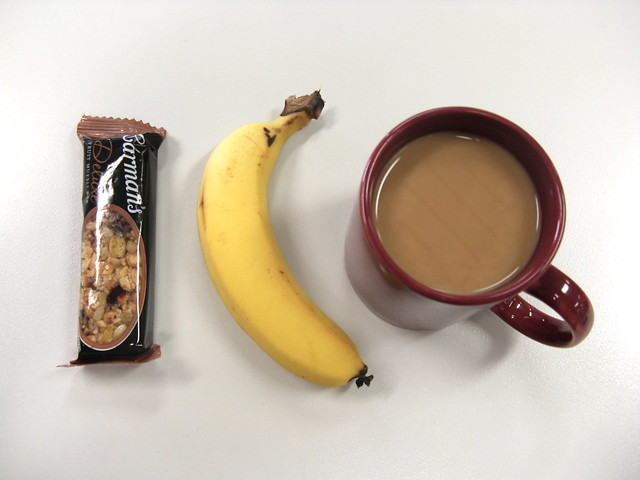
\includegraphics[width=\linewidth, height=2cm]{figs/472228.jpg}
%                 \vspace{-2mm}
%             \end{minipage}
%             & 
%             \begin{latin}
%             \begin{minipage}{.25\textwidth}
%                 \footnotesize
%                 \lr{Q: where is a banana?} \\
%                 \lr{A: a banana sits between a full coffee cup and a granola bar.}
%             \end{minipage}  
%         \end{latin}
%             & 
%             \begin{latin}
%             \begin{minipage}{.6\textwidth}
%                 \small
%                 \lr{LXMERT-3BiLSTM: a banana is on a table with a bowl of scissors.} \\
%                 \lr{VisualBERT-BahdanauLSTM: a banana sits on a of a a.}\\
%                 \lr{LXMERT-3Transformer: a banana sits on a table next to a table.}
%             \end{minipage}
%         \end{latin}
%             &
%             \begin{minipage} {0.05\textwidth}
%             \small        
%             WD \\ GE \\ WD
%             \end{minipage}
%             \\\hline
%             \begin{minipage}{.15\textwidth}
%                 \vspace*{2mm}
%                 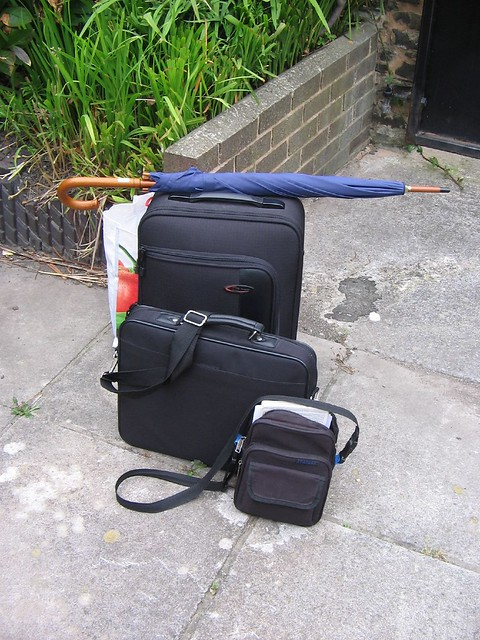
\includegraphics[width=\linewidth, height=2cm]{figs/485799.jpg}
%                 \vspace{-2mm}
%             \end{minipage}
%             & 
%             \begin{latin}
%             \begin{minipage}{.25\textwidth}
%                 \small
%                 \lr{Q: what color is the umbrella?} \\
%                 \lr{A: the umbrella is blue.}
%             \end{minipage}  
%         \end{latin}
%             & 
%             \begin{latin}
%             \begin{minipage}{.55\textwidth}
%                 \small
%                 \lr{LXMERT-3BiLSTM: the umbrella is blue.}\\
%                 \lr{VisualBERT-BahdanauLSTM: the umbrella is red.}\\
%                 \lr{LXMERT-3Transformer: the umbrella is blue.}
%             \end{minipage} 
%         \end{latin}
%             &
%             \begin{minipage} {0.05\textwidth}
%             \small
%             EM \\ WA \\ EM
%             \end{minipage}   
%             \\\hline
%              \begin{minipage}{.15\textwidth}
%                 \vspace*{2mm}
%                 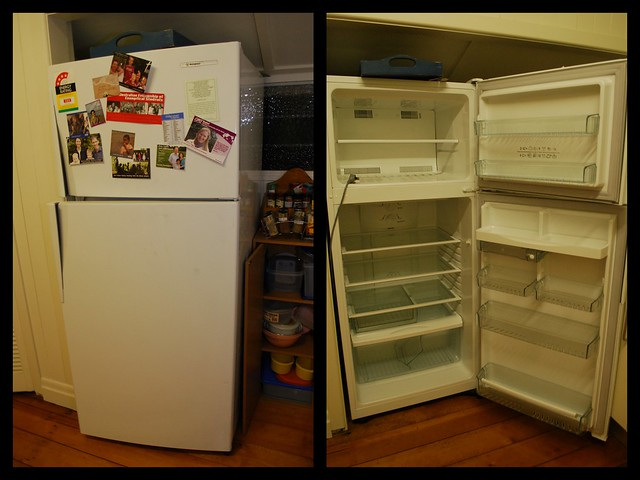
\includegraphics[width=\linewidth, height=2cm]{figs/571585.jpg}
%                 \vspace{-2mm}
%             \end{minipage}
%             & 
%             \begin{latin}
%             \begin{minipage}{.25\textwidth}
%                 \small
%                 \lr{Q: what kind of appliance is this?} \\
%                 \lr{A: this is refrigerator.}
%             \end{minipage}  
%         \end{latin}
%             & 
%             \begin{latin}
%             \begin{minipage}{.55\textwidth}
%                 \small
%                 \lr{LXMERT-3BiLSTM: refrigerator is pictured.} \\
%                 \lr{VisualBERT-BahdanauLSTM: this is blender.}\\
%                 \lr{LXMERT-3Transformer: this is refrigerator.}
%             \end{minipage}
%         \end{latin}
%             &
%             \begin{minipage} {0.05\textwidth}
%             \small
%             AA \\ E \\ EM
%             \end{minipage}  
%             \\ \hline
%           \end{tabular}
%           }
%       \caption{چند نمونه از پاسخ‌ها و اشتباهات آن‌ها بر اساس دسته‌بندی}
%       \label{table5}
%     \end{table}

%     تحلیل این 100 عضو نشان‌داد که تولید پاسخ‌ها باعث کاهش ابهام می‌شود. به عبارت
%     دیگر ارائه دادن توضیح اضافه بر کلمه پاسخ باعث می‌شود کاربر از اشتباهاتی
%     که سیتم ممکن است منجر بشود را آشکار می‌کند. برای مثال
%     فرض کنید پرسش و پاسخ‌های زیر تولید شده باشد:
%     \begin{latin}
%         \begin{itemize}
%             \itemsep-0.3em 
%             \item[] \small \lr{\textbf{Question}: Is the dog baring its teeth?}
%             \item[] \lr{\textbf{Reference}: No, the dog is not baring its teeth.}
%             \item[] \lr{\textbf{Generated}: Yes, the dog is \underline{grillening} its teeth.}
%         \end{itemize} 
%     \end{latin}
%     از آنجایی که کلمه 
%     \lr{grillening}
%     کلمه‌ای متناسب با حیوانات نیست و حیوانات قادر به انجام آن نیستند، می‌توان از 
%     این توضیح اشتباه به درست بودن پاسخ نیز شک کرد. از این رو ارائه توضیح اضافی 
%     منجر به رفع ابهامات در پرسش‌وپاسخ تصویری می‌شود. 

%     \begin{figure}[H]
%         \center{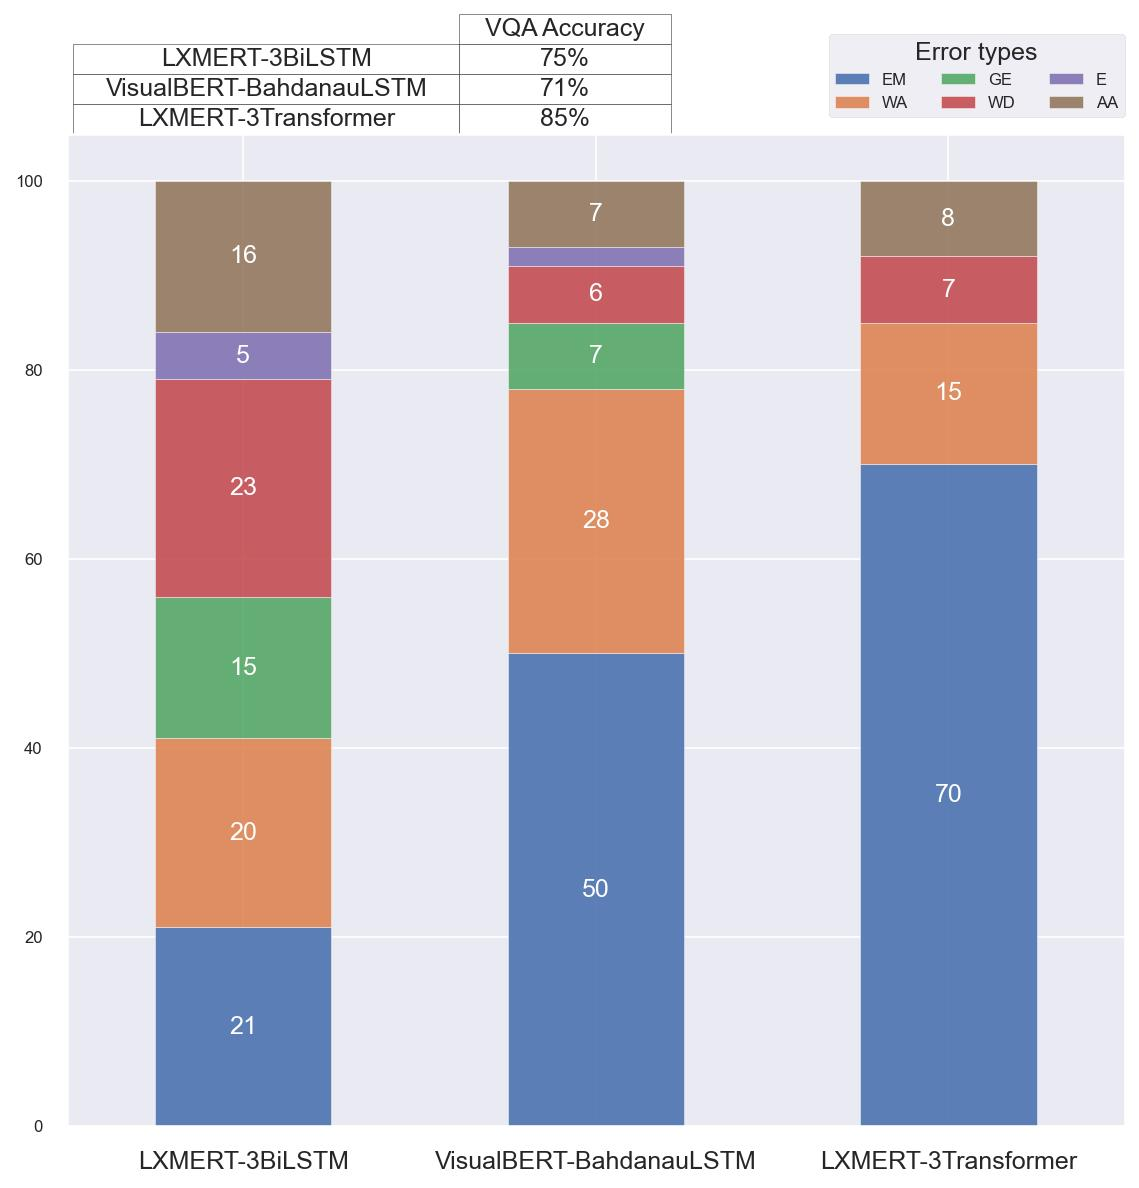
\includegraphics[width=0.7\textwidth]{figs/error.jpg}}
%         \caption{نتایج ارزیابی انسانی}
%         \label{fig:errors}
%     \end{figure}

%     شکل 
%     \ref{fig:errors}
%     نشان‌دهنده عملکرد خوب سیستم را نیز به خوبی نشان می‌دهد، به خصوص اینکه در 
%     حالت استفاده مدل‌های تبدیل‌شونده به عنوان کدگشا، هیچ اشتباه گرامری ندارد. 
%     یکی دیگر از نتایجی که می‌توان از این تحلیل‌ها گرفت، تاثیر کدگذار است که 
%     با توجه به دقت در پرسش‌وپاسخ تصویری، با حضور اشتباهات، همچنان مدلی که 
%     LXMERT
%     را به عنوان کدگذار استفاده کرده است، دارای دقت بیشتری از 
%     مدل‌های بر پایه 
%     VisualBERT
%     است. 
% }
% \section{جمع‌بندی}
% \paragraph{}
% {
%     با بررسی نتایج حاصل بر روی مجموعه داده 
%     FSVQA
%     و سیستم‌های ارائه شده می‌توان نتیجه گرفت استفاده از مدل‌های تبدیل‌شونده 
%     به عنوان کدگذار برای تولید پاسخ در پرسش‌وپاسخ تصویری عملکرد بسیار خوبی 
%     از خود نشان داده‌است. علاوه بر عملکرد خوب سیتم بر مجموعه داده، با ارزیابی انسانی 
%     ثابت شد ارائه دادن توضیح اضافی هنگام پاسخ باعث کمک بیشتر برای فهم پاسخ 
%     و حتی در حالاتی منجر به رفع ابهامات می‌شود. با این‌حال هم‌چنان مسیر بسیاری 
%     تا حل مسئله پرسش‌وپاسخ تصویری باقی‌مانده است. امتیازات بالایی که در این پژوهش بدست
%     آمده‌اند در واقع به علت ساده بودن مجموعه داده است و لازم است
%     پرسش‌هایی با پاسخ‌های طبیعی‌تر که از قوانین خاصی پیروی نمی‌کنند موجود
%     باشند تا بتوان مقادیر واقعی این معیارها را در محیط‌های واقعی‌تر محاسبه کرد.
% }
% !TeX root=main.tex

\chapter{نتیجه‌گیری و کارهای آینده} \label{ch:concl}
\thispagestyle{empty}


\section{نتیجه‌گیری}
\paragraph{}
{
      در ابتدا دیدیم که روش‌های زیادی برای پایش دستگاه‌های اینترنت اشیاء بصورت متمرکز و در مقایس بالا
      وجود ندارد. سپس با ارائه روش پیشنهادی، مشهاده شد که، با کمک کوبلت مجازی، پایش‌ دستگاه‌های اینترنت اشیاء
      در مقیاس بالا بسیار ساده خواهد بود. این روش به راحتی امکان پایش هزاران دستگاه اینترنت اشیاء در یک شهر را می‌دهد.
}

\section{دستاوردها}
\paragraph{}
{
      \begin{enumerate}
            \item پایش دستگاه‌های اینترنت اشیاء در مقیاس بالا
            \item استفاده از قراردادها و فناوری‌های شناخته شده و روش‌های متعارف و مرسوم
            \item سهولت اتصال دستگاه‌های اینترنت اشیاء به فضای ابری
            \item متمرکز شدن نرم‌افزار‌های معمول در کنار دستگاه‌های اینترنت اشیاء
      \end{enumerate}
}

\section{کارهای آینده}
\paragraph{}
{
      همانطور که در قسمت ارزیابی مشاهده شد، با وجود اعداد و ارقام معقول و مناسب، همچنان نمی‌توان ادعا کرد که 
      این مسئله حل شده است. هم‌چنین معماری‌های ارائه شده به نسبت قدیمی هستند و روش‌های بسیار نوآورانه‌تری معرفی 
      شده‌اند که می‌توانند این مسئله را با سادگی بیشتری حل کنند که در ادامه به آن‌ها می‌پردازیم.
}

\subsection{امنیت}
\label{subsec:security}
\paragraph{}
{
      در این پروژه درباره امنیت حرفی زده نشد. علت این امر هم این است که هدف پروژه امکانسنجی و پیاده‌سازی بوده است.
      امنیت بعنوان یک لایه روی معماری فعلی سوار شده. در چند بخش این مسئله را مورد بررسی قرار می‌دهیم:
      \begin{enumerate}
            \item امنیت ارتباط تامین‌کننده با کوبرنیتز
            \item امنیت ارتباط راط گرافیکی با تامین‌کننده
            \item امنیت ارتباط با دستگاه‌های اینترنت اشیاء
      \end{enumerate}

      در خصوص مورد اول، این مسئله حل شده است. بستر کوبرنیتز روش‌های مناسبی برای رمز‌نگاری داده‌ها و همچنین احراز هویت دارد و فقط باید در تامین‌کننده از آن‌ها استفاده نمود.
      \\
      مورد دوم و سوم اما جای کار دارد. باید سیستم احراز هویت در تامین کننده پیاده شده و از قراردادهای امن نظیر قرارداد امنیت لایه انتقال\footnote{\lr{Transport Layer Securty Protocol (TLS)}} استفاده شود.
}

\subsection{استفاده از فناوری‌های بروز تر}
\label{subsec:newer_tech}
\paragraph{}
{
      همانطور که در بخش
      \ref{sec:system_arch} به شرح معماری پرداخته شد سامانه پرداخته شد، 
      دیدیم که این معماری از قرارداد انتقال فرا متن استفاده کرده و جنس داده‌های ارسالی هم JSON می‌باشد. 
      مزیت استفاده از این فناوری، سادگی‌ آن است. اما قرارداد‌های بروزتری وجود دارند که کارایی سامانه را بالاتر می‌برند.
      برای مثال استفاده از \lr{gRPC} بجای قرارداد انتقال فرا متن. یا حتی استفاده از قرارداد \lr{websocket}.
}

\subsection{چارچوب}
\label{subsec:framework}
\paragraph{}
{
      همانطور که در بخش
      \ref{subsec:simulator} یک شبیه‌ساز ارائه شده،
      دیدیم که یک شبیه‌ برای نمایش نحوه کارکرد معماری ارائه شده.
      این به معنی است که برای استفاده از این روش، برنامه‌نویسان باید رابط‌های کاربردی قابل برنامه‌نویسی خود را
      پیاده‌سازی کرده و با معرفی آن از طریق کوبرنیتز به تامین کننده، امکان استفاده از این روش را داشته باشند.
      برای سهولت این امر، می‌توان چارچوبی\footnote{\lr{Framework}} ارائه کرد.
      در این چارچوب، بخش‌هایی وجود خواهد داشت که به برنامه‌نویسان امکان می‌دهد کد‌های خود در آن قرار داده و مسئولیت
      اجرا و برقراری ارتباط و امنیت را به چارچوب بسپارند.
}


\pagestyle{empty}
{
    % \settextfont[Scale=1,BoldFont={* Bold}]{Times New Roman}
    \setlatintextfont[Scale=0.8]{Times New Roman}
    \onehalfspacing
    % \bibliographystyle{acm-fa}%{chicago-fa}%{plainnat-fa}%
    \bibliographystyle{ieeetr-fa}%{chicago-fa}%{plainnat-fa}%
    % \bibliography{MyReferences}
}

\pagestyle{fancy}

% \appendix

% % !TeX root=main.tex
% دستورات زیر باید در اولین فایل پیوست باشند. آنها را حذف نکنید!
\addtocontents{toc}{
    \protect\renewcommand\protect\cftchappresnum{\appendixname~}%
    \protect\setlength{\cftchapnumwidth}{\mylenapp}}%
    
\chapter{مدیریت مراجع در لاتک}\label{App:RefMan}
\thispagestyle{empty}

در بخش \ref{Sec:Ref} اشاره شد که با دستور 
 \lr{\textbackslash bibitem}
  می‌توان یک مرجع را تعریف نمود و با فرمان
 \lr{\textbackslash cite}
  به آن ارجاع داد. این روش برای تعداد مراجع زیاد و تغییرات آنها مناسب نیست. در ادامه به صورت مختصر توضیحی در خصوص برنامه \lr{BibTeX} که همراه با توزیع‌های معروف تِک عرضه می‌شود و نحوه استفاده از آن در زی‌پرشین خواهیم داشت.

\section{ مدیریت مراجع با  \texorpdfstring{\lr{Bib\TeX}}{Bib\TeX} }
یکی از روش‌های قدرتمند و انعطاف‌پذیر برای نوشتن مراجع مقالات و مدیریت مراجع در لاتک، استفاده از  \lr{BibTeX} است.
 روش کار با  \lr{BibTeX} به این صورت است که مجموعه‌ی همه‌ی مراجعی را که در \پ استفاده کرده یا خواهیم کرد، 
در پرونده‌ی جداگانه‌ای نوشته و به آن فایل در سند خودمان به صورت مناسب لینک می‌دهیم.
 کنفرانس‌ها یا مجله‌های گوناگون برای نوشتن مراجع، قالب‌ها یا قراردادهای متفاوتی دارند که به آنها استیلهای مراجع گفته می‌شود.
 در این حالت به کمک ‌استیل‌های \lr{BibTeX} خواهید توانست تنها با تغییر یک پارامتر در پرونده‌ی ورودی خود، مراجع را مطابق قالب موردنظر تنظیم کنید. 
 بیشتر مجلات و کنفرانس‌های معتبر یک پرونده‌ی سبک (\lr{BibTeX Style}) با پسوند \lr{bst} در وب‌گاه خود می‌گذارند که برای همین منظور طراحی شده است.

به جز نوشتن مقالات این سبک‌ها کمک بسیار خوبی برای تهیه‌ی مستندات علمی همچون پایان‌نامه‌هاست که فرد می‌تواند هر قسمت از کارش را که نوشت مراجع مربوطه را به بانک مراجع خود اضافه نماید. با داشتن چنین بانکی از مراجع، وی خواهد توانست به راحتی یک یا چند ارجاع به مراجع و یا یک یا چند بخش را حذف یا اضافه ‌نماید؛ 
مراجع به صورت خودکار مرتب شده و فقط مراجع ارجاع داده شده در قسمت کتاب‌نامه خواهندآمد. قالب مراجع به صورت یکدست مطابق سبک داده شده بوده و نیازی نیست که کاربر درگیر قالب‌دهی به مراجع باشد. 
در این جا مجموعه‌ سبک‌های بسته \lr{Persian-bib} که برای  زی‌پرشین آماده شده‌اند به صورت مختصر معرفی شده و روش کار با آن‌ها گفته می‌شود. برای اطلاع بیشتر به راهنمای بسته‌ی \lr{Persian-bib} مراجعه فرمایید.
\subsection{سبک‌های فعلی قابل استفاده در زی‌پرشین}
در حال حاضر فایلهای سبک زیر برای استفاده در زی‌پرشین آماده شده‌اند:

\singlespacing
\begin{description}
\item [unsrt-fa.bst] این سبک متناظر با \lr{unsrt.bst} می‌باشد. مراجع به ترتیب ارجاع در متن ظاهر می‌شوند.
\item [plain-fa.bst] این سبک متناظر با \lr{plain.bst} می‌باشد. مراجع بر اساس نام‌خانوادگی نویسندگان، به ترتیب صعودی مرتب می‌شوند.
 همچنین ابتدا مراجع فارسی و سپس مراجع انگلیسی خواهند آمد.
\item [acm-fa.bst] این سبک متناظر با \lr{acm.bst} می‌باشد. شبیه \lr{plain-fa.bst} است.  قالب مراجع کمی متفاوت است. اسامی نویسندگان انگلیسی با حروف بزرگ انگلیسی نمایش داده می‌شوند. (مراجع مرتب می‌شوند)
\item [ieeetr-fa.bst] این سبک متناظر با \lr{ieeetr.bst} می‌باشد. (مراجع مرتب نمی‌شوند)
\item [plainnat-fa.bst] این سبک متناظر با \lr{plainnat.bst} می‌باشد. نیاز به بستهٔ \lr{natbib} دارد. (مراجع مرتب می‌شوند)
\item [chicago-fa.bst] این سبک متناظر با \lr{chicago.bst} می‌باشد. نیاز به بستهٔ \lr{natbib} دارد. (مراجع مرتب می‌شوند)
\item [asa-fa.bst] این سبک متناظر با \lr{asa.bst} می‌باشد. نیاز به بستهٔ \lr{natbib} دارد. (مراجع مرتب می‌شوند)
\end{description}
\doublespacing

با استفاده از استیلهای فوق می‌توانید به انواع مختلفی از مراجع فارسی و لاتین ارجاع دهید. به عنوان نمونه مرجع 
\cite{Omidali82phdThesis}
 یک نمونه پروژه دکترا (به فارسی) و مرجع 
\cite{Vahedi87} یک نمونه مقاله مجله فارسی است.
مرجع 
\cite{Amintoosi87afzayesh}  یک نمونه  مقاله کنفرانس فارسی و
مرجع 
\cite{Pedram80osool} یک نمونه کتاب فارسی با ذکر مترجمان و ویراستاران فارسی است. مرجع 
\cite{Khalighi07MscThesis} یک نمونه پروژه کارشناسی ارشد انگلیسی و
\cite{Khalighi87xepersian} هم یک نمونه متفرقه  می‌باشند.

مراجع 
\cite{Gonzalez02book,Baker02limits} 
نمونه کتاب و مقاله انگلیسی هستند.
استیل مورد استفاده در این \پ \lr{acm-fa} است که خروجی آنرا در بخش مراجع می‌توانید مشاهده کنید.
نمونه  خروجی سبک \lr{asa-fa} در شکل \ref{fig:asafa} آمده است.

\begin{figure}[t]
\centering
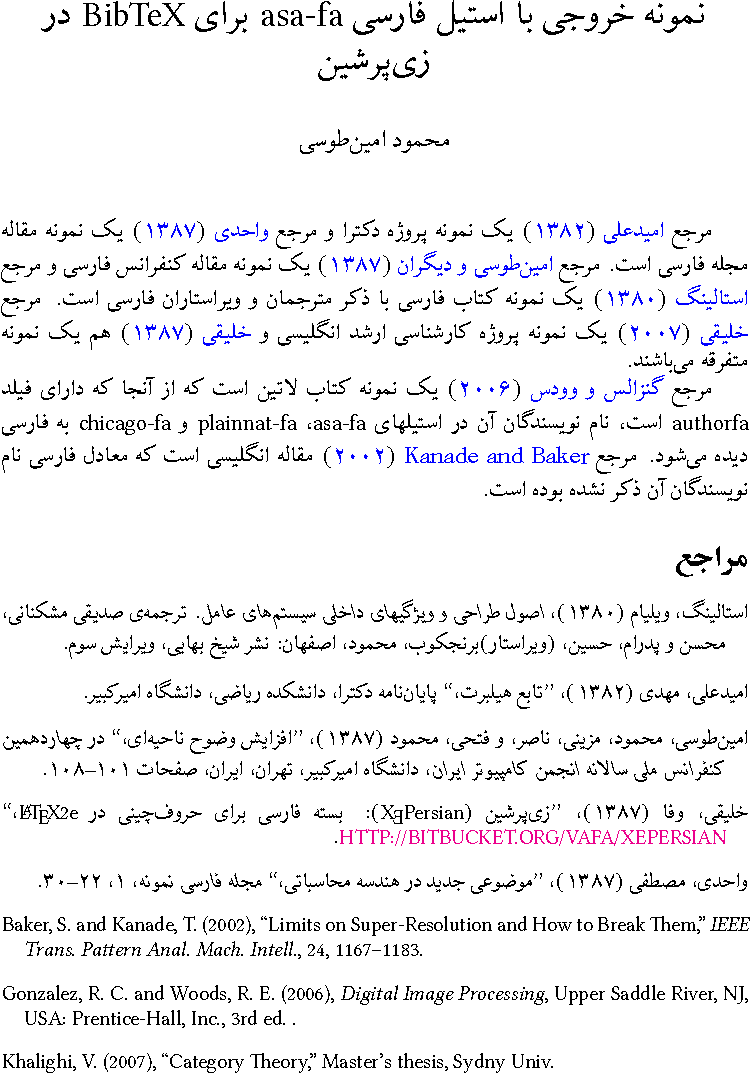
\includegraphics[width=.8\textwidth]{asa-fa-crop.pdf}
\caption{نمونه خروجی با سبک \lr{asa-fa}}
\label{fig:asafa}
\end{figure} 

\subsection{ نحوه استفاده از سبک‌های فارسی}


برای استفاده از بیب‌تک باید مراجع خود را در یک فایل با پسوند \lr{bib} ذخیره نمایید. یک فایل \lr{bib} در واقع یک پایگاه داده از مراجع\LTRfootnote{Bibliography Database}  شماست که هر مرجع در آن به عنوان یک رکورد از این پایگاه داده
با قالبی خاص ذخیره می‌شود. به هر رکورد یک مدخل\LTRfootnote{Entry} گفته می‌شود. یک نمونه مدخل برای معرفی کتاب \lr{Digital Image Processing} در ادامه آمده است:

\singlespacing
\begin{LTR}
\begin{verbatim}
@BOOK{Gonzalez02image,
  AUTHOR =      {Rafael Gonzalez and Richard Woods},
  TITLE =       {Digital Image Processing},
  PUBLISHER =   {Prentice-Hall, Inc.},
  YEAR =        {2006},
  EDITION =     {3rd},
  ADDRESS =     {Upper Saddle River, NJ, USA}
}
\end{verbatim}
\end{LTR}
\doublespacing

در مثال فوق، \lr{@BOOK} مشخصه‌ی شروع یک مدخل مربوط به یک کتاب و \lr{Gonzalez02book} برچسبی است که به این مرجع منتسب شده است.
 این برچسب بایستی یکتا باشد. برای آنکه فرد به راحتی بتواند برچسب مراجع خود را به خاطر بسپارد و حتی‌الامکان برچسب‌ها متفاوت با هم باشند معمولاً از قوانین خاصی به این منظور استفاده می‌شود. یک قانون می‌تواند فامیل نویسنده‌ی اول+دورقم سال نشر+اولین کلمه‌ی عنوان اثر باشد. به \lr{AUTHOR} و $\dots$ و \lr{ADDRESS} فیلدهای این مدخل گفته می‌شود؛ که هر یک با مقادیر مربوط به مرجع مقدار گرفته‌اند. ترتیب فیلدها مهم نیست. 

انواع متنوعی از مدخل‌ها برای اقسام مختلف مراجع همچون کتاب، مقاله‌ی کنفرانس و مقاله‌ی ژورنال وجود دارد که برخی فیلدهای آنها با هم متفاوت است. 
نام فیلدها بیانگر نوع اطلاعات آن می‌باشد. مثالهای ذکر شده در فایل \lr{MyReferences.bib} کمک خوبی به شما خواهد بود. 
%این فایل یک فایل متنی بوده و با ویرایشگرهای معمول همچون \lr{Notepad++} قابل ویرایش می‌باشد. برنامه‌هایی همچون 
%\lr{TeXMaker}
% امکاناتی برای نوشتن این مدخل‌ها دارند و به صورت خودکار فیلدهای مربوطه را در فایل \lr{bib}  شما قرار می‌دهند.  
با استفاده از سبک‌های فارسی آماده شده، محتویات هر فیلد می‌تواند به فارسی نوشته شود، ترتیب مراجع و نحوه‌ی چینش فیلدهای هر مرجع را سبک مورد استفاده  مشخص خواهد کرد.

نکته: بدون اعمال تنظیمات موردنیاز \lr{Bib\TeX} در \lr{TeXWorks}، مراجع فارسی در استیل‌هایی که مراجع را به صورت مرتب شده چاپ می‌کنند، ترتیب کاملاً درستی نخواهند داشت. برای توضیحات بیشتر \cite{persianbib87userguide} را ببینید یا به سایت پارسی‌لاتک مراجعه فرمایید. تنظیمات موردنیاز در \lr{TeXMaker} اصلاح شده اعمال شده‌اند.

\textbf{برای درج مراجع خود لازم نیست نگران موارد فوق باشید. در فایل 
\lr{MyReferences.bib}
 که همراه با این \پ هست، موارد مختلفی درج شده است و کافیست مراجع خود را جایگزین موارد مندرج در آن نمایید.
}

پس از قرار دادن مراجع خود، یک بار \lr{XeLaTeX} را روی سند خود اجرا نمایید، سپس \lr{bibtex} و پس از آن دوبار \lr{XeLaTeX} را. در \lr{TeXMaker} کلید \lr{F11} و در \lr{TeXWorks} هم گزینه‌ی \lr{BibTeX} از منوی \lr{Typeset}، \lr{BibTeX} را روی سند شما اجرا می‌کنند.

برای بسیاری از مقالات لاتین حتی لازم نیست که مدخل مربوط به آنرا خودتان بنویسید. با جستجوی نام مقاله + کلمه \lr{bibtex}  در اینترنت سایتهای بسیاری همچون \lr{ACM} و \lr{ScienceDirect} را خواهید یافت که مدخل \lr{bibtex} مربوط به مقاله شما را دارند و کافیست آنرا به انتهای فایل \lr{MyReferences} اضافه کنید.

از هر یک از سبکهای \lr{Persian-bib} می‌توانید استفاده کنید، البته اگر از سه استیل آخر استفاده می‌کنید و مایلید که مراجع شما شماره بخورند باید بسته \lr{natbib} را با گزینه \lr{numbers} فراخوانی نمایید.

% % !TeX root=main.tex

\chapter{‌جدول، نمودار و الگوریتم در لاتک}\label{App:Latex:More}
\thispagestyle{empty}

در این بخش نمونه مثالهایی از جدول، نمودار و الگوریتم در لاتک را خواهیم دید.
\section{مدلهای حرکت دوبعدی}
بسیاری از اوقات حرکت بین دو تصویر از یک صحنه با یکی از مدلهای پارامتری ذکر شده در جدول \eqref{tab:MotionModels} قابل مدل نمودن می‌باشد.  
\begin{table}[ht]
\caption{مدلهای تبدیل.}
\label{tab:MotionModels}
\centering
\onehalfspacing
\begin{tabular}{|r|c|l|r|}
\hline نام مدل & درجه آزادی & تبدیل مختصات & توضیح \\ 
\hline انتقالی & ۲ & $\begin{aligned} x'=x+t_x \\ y'=y+t_y \end{aligned}$  &  انتقال دوبعدی\\ 
\hline اقلیدسی & ۳ & $\begin{aligned} x'=xcos\theta - ysin\theta+t_x \\ y'=xsin\theta+ycos\theta+t_y \end{aligned}$  &  انتقالی+دوران \\ 
\hline مشابهت & ۴ & $\begin{aligned} x'=sxcos\theta - sysin\theta+t_x \\ y'=sxsin\theta+sycos\theta+t_y  \end{aligned}$  & اقلیدسی+تغییرمقیاس \\ 
\hline آفین & ۶ & $\begin{aligned} x'=a_{11}x+a_{12}y+t_x \\ y'=a_{21}x+a_{22}y+t_y \end{aligned}$  & مشابهت+اریب‌شدگی \\ 
\hline  پروجکتیو & ۸ & $\begin{aligned} x'&=(m_1x+m_2y+m_3)/D \\ y'&=(m_4x+m_5y+m_6)/D \\ D&=m_7x+m_8y+1 \end{aligned}$  & آفین+\lr{keystone+chirping} \\ 
\hline  شارنوری & $\infty $ & $\begin{aligned} x'=x+v_x(x,y) \\ y'=y+v_y(x,y) \end{aligned}$  &  حرکت آزاد\\ 
\hline 
\end{tabular} 
\end{table}

\section{ماتریس}

شناخته‌شده‌ترین روش تخمین ماتریس هوموگرافی الگوریتم تبدیل خطی مستقیم (\lr{DLT\LTRfootnote{Direct Linear Transform}}) است.  فرض کنید چهار زوج نقطهٔ متناظر در دو تصویر در دست هستند،  $\mathbf{x}_i\leftrightarrow\mathbf{x}'_i$   و تبدیل با رابطهٔ
  $\mathbf{x}'_i = H\mathbf{x}_i$
  نشان داده می‌شود که در آن:
\[\mathbf{x}'_i=(x'_i,y'_i,w'_i)^\top  \]
و
\[ H=\left[
\begin{array}{ccc}
h_1 & h_2 & h_3 \\ 
h_4 & h_5 & h_6 \\ 
h_7 & h_8 & h_9
\end{array} 
\right]\]
رابطه زیر را برای الگوریتم  \eqref{alg:DLT} لازم دارم.
\begin{equation}\label{eq:DLT_Ah}
\left[
\begin{array}{ccc}
0^\top & -w'_i\mathbf{x}_i^\top & y'_i\mathbf{x}_i^\top \\ 
w'_i\mathbf{x}_i & 0^\top & -x'_i\mathbf{x}_i^\top \\ 
- y'_i\mathbf{x}_i^\top & x'_i\mathbf{x}_i^\top & 0^\top
\end{array} 
\right]
\left(
\begin{array}{c}
\mathbf{h}^1 \\ 
\mathbf{h}^2 \\ 
\mathbf{h}^3
\end{array} 
\right)=0
\end{equation}

\section{الگوریتم با دستورات فارسی}
با مفروضات فوق، الگوریتم \lr{DLT} به صورت نشان داده شده در الگوریتم \eqref{alg:DLT}  خواهد بود.
\begin{algorithm}[t]
\onehalfspacing
\caption{الگوریتم \lr{DLT} برای تخمین ماتریس هوموگرافی.} \label{alg:DLT}
\begin{algorithmic}[1]
\REQUIRE $n\geq4$ زوج نقطهٔ متناظر در دو تصویر 
${\mathbf{x}_i\leftrightarrow\mathbf{x}'_i}$،\\
\ENSURE ماتریس هوموگرافی $H$ به نحوی‌که: 
$\mathbf{x}'_i = H \mathbf{x}_i$.
  \STATE برای هر زوج نقطهٔ متناظر
$\mathbf{x}_i\leftrightarrow\mathbf{x}'_i$ 
ماتریس $\mathbf{A}_i$ را با استفاده از رابطهٔ \ref{eq:DLT_Ah} محاسبه کنید.
  \STATE ماتریس‌های ۹ ستونی  $\mathbf{A}_i$ را در قالب یک ماتریس $\mathbf{A}$ ۹ ستونی ترکیب کنید. 
  \STATE تجزیهٔ مقادیر منفرد \lr{(SVD)}  ماتریس $\mathbf{A}$ را بدست آورید. بردار واحد متناظر با کمترین مقدار منفرد جواب $\mathbf{h}$ خواهد بود.
  \STATE  ماتریس هوموگرافی $H$ با تغییر شکل $\mathbf{h}$ حاصل خواهد شد.
\end{algorithmic}
\end{algorithm}

\section{الگوریتم با دستورات لاتین}
الگوریتم \ref{alg:RANSAC} یک الگوریتم با دستورات لاتین است.

\begin{algorithm}[t]
\onehalfspacing
\caption{الگوریتم \lr{RANSAC} برای تخمین ماتریس هوموگرافی.} \label{alg:RANSAC}
\begin{latin}
\begin{algorithmic}[1]
\REQUIRE $n\geq4$ putative correspondences, number of estimations, $N$, distance threshold $T_{dist}$.\\
\ENSURE Set of inliers and Homography matrix $H$.
\FOR{$k = 1$ to $N$}
  \STATE Randomly choose 4 correspondence,
  \STATE Check whether these points are colinear, if so, redo the above step
  \STATE Compute the homography $H_{curr}$ by DLT algorithm from the 4 points pairs,
  \STATE $\ldots$ % الگوریتم کامل نیست
  \ENDFOR
  \STATE Refinement: re-estimate H from all the inliers using the DLT algorithm.
\end{algorithmic}
\end{latin}
\end{algorithm}

\section{نمودار}
لاتک بسته‌هایی با قابلیت‌های زیاد برای رسم انواع مختلف نمودارها دارد. مانند بسته‌های \lr{Tikz} و  \lr{PSTricks}. توضیح اینها فراتر از این پیوست کوچک است. مثالهایی از رسم نمودار را در مجموعه پارسی‌لاتک خواهید یافت. توصیه می‌کنم که حتماً مثالهایی از برخی از آنها را ببینید. راهنمای همه آنها در تک‌لایو هست. نمونه مثالهایی از بسته \lr{Tikz} را می‌توانید در \url{http://www.texample.net/tikz/examples/} ببینید.

\section{تصویر}
نمونه تصاویری در بخش قبل دیدیم. دو تصویر شیر کنار هم را هم در شکل \ref{fig:twolion} مشاهده می‌کنید.
\begin{figure}[t]
\centering 
\subfigure[شیر ۱]{ \label{fig:twolion:one}

\includegraphics[width=.3\textwidth]{lion}}
%\hspace{2mm}
\subfigure[شیر ۲]{ \label{fig:twolion:two}

\includegraphics[width=.3\textwidth]{lion}}
\caption{دو شیر}
\label{fig:twolion} %% label for entire figure
\end{figure}

%\baselineskip=.75cm
\onehalfspacing
\chapter*{واژه‌نامه فارسی به انگلیسی}\markboth{واژه‌نامه فارسی به انگلیسی}{واژه‌نامه فارسی به انگلیسی}
\addcontentsline{toc}{chapter}{واژه‌نامه فارسی به انگلیسی}
\thispagestyle{empty}
\englishgloss{Worker Pool}{استخر کارگران}
\englishgloss{Cloud Environment}{بستر ابری}
\englishgloss{Kubernetes}{کوبرنیتز}
\englishgloss{Containers}{کانتینرها}
\englishgloss{Cloud Native Computing Foundation}{بنیاد CNCF}
\englishgloss{Cloud Environment}{بسترهای ابری}
\englishgloss{Distributed Environment}{محیط‌های توزیع شده}
\englishgloss{Virtual Machine}{خدمت دهنده‌ مجازی}
\englishgloss{Physical Server}{فیزیکی}
\englishgloss{automation}{اتوماسیون}
\englishgloss{Load Balancing}{، توازن بار}
\englishgloss{Automatic Diagnostics}{و تشخیص خودکار اشکال}
\englishgloss{Docker}{داکر}
\englishgloss{Pod}{پاد‌}
\englishgloss{Node}{گره‌}
\englishgloss{Kublet}{کوبلت}
\englishgloss{Kube-proxy}{پروکسی}
\englishgloss{Kube-controller-manager}{کنترل‌کننده کوبرنیتز}
\englishgloss{Kube-scheduler}{برنامه‌ریز کوبرنیتز}
\englishgloss{Shared Memory}{حافظه مشترک}
\englishgloss{Cluster}{خوشه}
\englishgloss{Monitoring}{پایش}
\englishgloss{Kubernetes Cluster}{خوشه کوبنیتز}
\englishgloss{Hypertext Transfer Protocol (HTTP)}{قرارداد انتقال فرامتن}
\englishgloss{HTTP Methods}{توابع قرارداد انتقال فرا متن}
\englishgloss{GET}{دریافت}
\englishgloss{POST}{ساخت}
\englishgloss{PUT}{بروزرسانی}
\englishgloss{DELETE}{حذف}
\englishgloss{PATCH}{بروزرسانی مقطعی}
\englishgloss{HTTP Request}{درخواست قرارداد انتقال فرا متن}
\englishgloss{HTTP Response}{پاسخ قرارداد انتقال فرا متن}
\englishgloss{Uniform Resource Locator}{آدرس}
\englishgloss{Path}{مسیر}
\englishgloss{Domain}{دامنه}
\englishgloss{Request Body}{بدنه درخواست}
\englishgloss{Status Code}{کد وضعیت}
\englishgloss{Response Body}{محتوای پاسخ}
\englishgloss{Representational State Transfer (REST)}{انتقال حالت نمایشی}
\englishgloss{Resources}{منابع}
\englishgloss{Uniform Interface}{یکپارچگی}
\englishgloss{Application Programming Interface}{رابط کاربردی قابل برنامه‌ریزی}
\englishgloss{Virtual Kubelet}{کوبلت مجازی}
\englishgloss{Integration}{ادغام}
\englishgloss{Workloads}{کارها}
\englishgloss{Scheduler}{برنامه‌ریز}
\englishgloss{Internt of Things (IoT)}{اینترنت اشیاء}
\englishgloss{Callback-Based Software}{نرم‌افزارهای مبتنی بر بازخوانی}
\englishgloss{Callback}{بازخوانی}
\englishgloss{Transport Layer Securty Protocol (TLS)}{امنیت لایه انتقال}
\englishgloss{Framework}{چارچوب}
\englishgloss{Message Queuing Telemetry Transport Protocol}{MQTT قرارداد}
\englishgloss{Constrained Application Protocol}{CoAP قرارداد}
\englishgloss{Blockchain}{زنجیره‌ی بلوکی} 
\englishgloss{Provider}{تامین‌کننده}
\englishgloss{Controller}{کنترلکننده}
\englishgloss{Device}{دستگاهها}
\chapter*{واژه‌نامه  انگلیسی به  فارسی \label{ch:en2fa}}\markboth{واژه‌نامه  انگلیسی به  فارسی}{واژه‌نامه  انگلیسی به  فارسی}
\addcontentsline{toc}{chapter}{واژه‌نامه  انگلیسی به  فارسی}
\thispagestyle{empty}
\persiangloss{گره}{Node}
\persiangloss{خدمت گیرنده}{Client}
\persiangloss{خدمت دهنده}{Server}
\persiangloss{قرارداد}{Protocol}
\persiangloss{رابط}{Interface}
\persiangloss{رابط کاربردی قابل برنامه‌نویسی}{Application Programming Interface}
\persiangloss{قرارداد انتقال فرا متن}{Hypertext Transfer Protocol}
\persiangloss{پشتوانه}{Backend}
\persiangloss{بازخوانی}{Callback}
% \persiangloss{TODO}{بقیش بعدا}
% \persiangloss{پرسش‌و‌پاسخ تصویری}{Visual Question Answering}
% \persiangloss{یادگیری عمیق}{Deep Learning}
% \persiangloss{توجه}{Attention}
% \persiangloss{یادگیری انتقالی}{Transfer Learning}
% \persiangloss{خطا}{Error}
% \persiangloss{مشخصات}{Specification}
% \persiangloss{یادگیری بازنمایی}{Representation Learning}
% \persiangloss{شبکه عصبی بازگشتی}{Recurrent Neural Network}
% \persiangloss{کدگذار}{Encoder}
% \persiangloss{کدگشا}{Decoder}
% \persiangloss{دنباله‌به‌دنباله}{Sequence-to-Sequence}
% \persiangloss{انتها به انتها}{End-to-End}
% \persiangloss{تبدیل‌شونده}{Transformer}
% \persiangloss{نشانه‌گذاری}{Tokenization}
% \persiangloss{تعبیه}{Embedding}
% \persiangloss{کلید}{Key}
% \persiangloss{پرسش}{Query}
% \persiangloss{مقدار}{Value}
% \persiangloss{توجه چندسر}{Multi-Head Attention}
% \persiangloss{مدل زبانی ماسک‌دار}{Masked Language Model}
% \persiangloss{گسترش رو به جلو}{Forward Propagation}
% \persiangloss{گرادیان کاهشی}{Gradient Decent}
% \persiangloss{توجه به خود}{Self-attention}
% \persiangloss{مدل تک‌جریان}{Single-stream model}
% \persiangloss{مدل دوجریان}{Dual-stream model}
% \persiangloss{شباهت نحوی}{Word-similarity}
% \persiangloss{ارزیابی انسانی}{Human Evaluation}
\printindex
% !TeX root=main.tex
% در این فایل، عنوان پایان‌نامه، مشخصات خود و چکیده پایان‌نامه را به انگلیسی، وارد کنید.

%%%%%%%%%%%%%%%%%%%%%%%%%%%%%%%%%%%%
\baselineskip=.6cm
\begin{latin}
\latinuniversity{Iran University of Science and Technology}
\latinfaculty{Computer Engineering Department}
\latinsubject{Computer Engineering - Software Engineering}
\latinfield{Software Engineering}
\latintitle{A K8-Based Mechanism for Remote Monitoring and Control of IoT Devices}
\firstlatinsupervisor{Dr. Mohsen Sharifi}
%\secondlatinsupervisor{Second Supervisor}
% \firstlatinadvisor{First Advisor}
%\secondlatinadvisor{Second Advisor}
\latinname{Sina}
\latinsurname{Shabani Kumeleh}
\latinthesisdate{Summer 2023}
\latinkeywords{Internet of Things, Kubernetes, Virtual Kubelet, Centeralized Monitoring, Scalable Monitoring}
\en-abstract{
  In today's world, the management, control and supervision of IoT devices 
  face a significant challenge. The lack of a unified solution hinders 
  effective control and monitoring of a diverse range of IoT devices. 
  This results in fragmented control mechanisms and complex management processes. 
  The project 
  "A K8-Based Mechanism for Remote Monitoring and Control of IoT Devices" 
  proposes an innovative approach to address this challenge. 
  By leveraging the capabilities of Kubernetes as the core infrastructure, 
  the project aims to provide a comprehensive solution for centralized control
   and monitoring of IoT devices. This solution streamlines the management 
   process and enhances efficiency by offering a unified platform for device 
   control and monitoring. With its robust architecture, the project facilitates
    seamless integration, scalability, and intelligent decision-making based on
     real-time device data. By implementing this solution, organizations can
      effectively manage and monitor their IoT device ecosystem while optimizing
       operations and ensuring optimal performance.
}
\latinfirstPage
\end{latin}

\label{LastPage}

\end{document}
